\documentclass[aos,preprint]{imsart}

%% Packages
\RequirePackage{amsthm,amsmath,amsfonts,amssymb,multirow,bbm}
%\RequirePackage[numbers]{natbib}
\RequirePackage[authoryear]{natbib} %% uncomment this for author-year bibliography
\RequirePackage[colorlinks,citecolor=blue,urlcolor=blue]{hyperref}
\RequirePackage{graphicx,graphics,epstopdf}

\startlocaldefs
%%%%%%%%%%%%%%%%%%%%%%%%%%%%%%%%%%%%%%%%%%%%%%
%%                                          %%
%% Uncomment next line to change            %%
%% the type of equation numbering           %%
%%                                          %%
%%%%%%%%%%%%%%%%%%%%%%%%%%%%%%%%%%%%%%%%%%%%%%
%\numberwithin{equation}{section}
%%%%%%%%%%%%%%%%%%%%%%%%%%%%%%%%%%%%%%%%%%%%%%
%%                                          %%
%% For Axiom, Claim, Corollary, Hypothezis, %%
%% Lemma, Theorem, Proposition              %%
%% use \theoremstyle{plain}                 %%
%%                                          %%
%%%%%%%%%%%%%%%%%%%%%%%%%%%%%%%%%%%%%%%%%%%%%%
%\theoremstyle{plain}
\newtheorem{axiom}{Axiom}
\newtheorem{claim}[axiom]{Claim}
\newtheorem{theorem}{Theorem}[section]
\newtheorem{lemma}[theorem]{Lemma}
\newtheorem{assumption}[theorem]{Assumption}
%%%%%%%%%%%%%%%%%%%%%%%%%%%%%%%%%%%%%%%%%%%%%%
%%                                          %%
%% For Assumption, Definition, Example,     %%
%% Notation, Property, Remark, Fact         %%
%% use \theoremstyle{remark}                %%
%%                                          %%
%%%%%%%%%%%%%%%%%%%%%%%%%%%%%%%%%%%%%%%%%%%%%%
\theoremstyle{remark}
\newtheorem{definition}[theorem]{Definition}
\newtheorem*{remark}{Remark}
\newtheorem*{example}{Example}
\newtheorem*{fact}{Fact}
%%%%%%%%%%%%%%%%%%%%%%%%%%%%%%%%%%%%%%%%%%%%%%
%% Please put your definitions here:        %%
%%%%%%%%%%%%%%%%%%%%%%%%%%%%%%%%%%%%%%%%%%%%%%

\endlocaldefs

\begin{document}

\begin{frontmatter}
\title{Manifold fitting by ridge estimation: A local KDE approach}
%\title{A sample article title with some additional note\thanksref{t1}}
\runtitle{Manifold fitting by ridge estimation: A local KDE approach}
%\thankstext{T1}{A sample additional note to the title.}

\begin{aug}
%%%%%%%%%%%%%%%%%%%%%%%%%%%%%%%%%%%%%%%%%%%%%%
%%Only one address is permitted per author. %%
%%Only division, organization and e-mail is %%
%%included in the address.                  %%
%%Additional information can be included in %%
%%the Acknowledgments section if necessary. %%
%%%%%%%%%%%%%%%%%%%%%%%%%%%%%%%%%%%%%%%%%%%%%%
\author{\fnms{Zhigang} \snm{Yao}\thanksref{t1}\ead[label=e1]{zhigang.yao@nus.edu.sg}},
\and
\author{\fnms{Zheng} \snm{Zhai}\thanksref{t2} \ead[label=e2]{stazhai@nus.edu.sg}}
\thankstext{t1}{Supported by the MOE Tier 1 R-155-000-210-114 and Tier 2 R-155-000-184-112 at National University of Singapore}
\thankstext{t2}{Correspondence can be addressed to: zhigang.yao@nus.edu.sg or stazhai@nus.edu.sg}
%\and
%\author[B]{\fnms{Third} \snm{Author}\ead[label=e3]{third@somewhere.com}}
%%%%%%%%%%%%%%%%%%%%%%%%%%%%%%%%%%%%%%%%%%%%%%
%% Addresses                                %%
%%%%%%%%%%%%%%%%%%%%%%%%%%%%%%%%%%%%%%%%%%%%%%
\affiliation{National University of Singapore}
%\address[A,B]{National University of Singapore} 
%\printead{e1,e2}
%}

%\address[B]{Department,
%University or Company Name,
%\printead{e2,e3}}
\end{aug}

%\begin{aug}
%\author{\fnms{First} \snm{Author}\thanksref{t1,t2}\ead[label=e1]{first@somewhere.com}},
%\author{\fnms{Second} \snm{Author}\thanksref{t3}\ead[label=e2]{second@somewhere.com}}
%\and
%\author{\fnms{Third} \snm{Author}\thanksref{t1}
%\ead[label=e3]{third@somewhere.com}
%\ead[label=u1,url]{http://www.foo.com}}
%
%\thankstext{t1}{Some comment}
%\thankstext{t2}{First supporter of the project}
%\thankstext{t3}{Second supporter of the project}
%\runauthor{F. Author et al.}
%
%\affiliation{Some University and Another University}
%
%\address{Address of the First and Second authors\\
%usually few lines long\\
%\printead{e1}\\
%\phantom{E-mail:\ }\printead*{e2}}
%
%\address{Address of the Third author\\
%usually few lines long\\
%usually few lines long\\
%\printead{e3}\\
%\printead{u1}}
%\end{aug}

\begin{abstract}
In this paper, we aim to obtain a new ridge which is more closer to the hidden manifold. To accomplish our goal, we mainly work in two perspectives. Firstly, to reduce the derivatives' estimation error, we consider LKDE (a local version of the KDE (kernel density estimation)) approach to estimate the density ridge. Meanwhile, we provide a theoretical analysis to show that this new local approach could be used to reduce the bias more effectively than the classical KDE approach. Secondly, we analyze the eigen-space of the Hessian matrix with the shifting position of $x$ and show the necessity of nonlinear transformation composed with the KDE function. By applying the nonlinear transformation, we will get a high quality ridge which is a subset of the original one. Numerical experiments indicate that the ridge obtained from our local KDE approach does indeed have a smaller average margin and Hausdorff distance to the hidden manifold than other related algorithms.
\end{abstract}


%\begin{keyword}[class=MSC2010]
%\kwd[Primary ]{00X00}
%\kwd{00X00}
%\kwd[; secondary ]{00X00}
%\end{keyword}
%
%\begin{keyword}
%\kwd{Manifold Fitting}
%\kwd{Ridge estimation}
%\kwd{Kernel density estimation}
%\kwd{Derivatives estimation}
%\end{keyword}

\end{frontmatter}

\begin{quote}
{\bf Keywords}:    Manifold Fitting, Ridge Estimation, Kernel Density Estimation, Derivatives Estimation, Rank-one Modification
\end{quote}
\begin{quote} \small
{\bf AMS 2000 subject classifications}:   Primary 62G05;
secondary 62G32.
\end{quote}

%%%%%%%%%%%%%%%%%%%%%%%%%%%%%%%%%%%%%%%%%%%%%%
%% Please use \tableofcontents for articles %%
%% with 50 pages and more                   %%
%%%%%%%%%%%%%%%%%%%%%%%%%%%%%%%%%%%%%%%%%%%%%%
%\tableofcontents

\section{Introduction}

Today, dealing with high-dimensional data is often costly, as it has required the exponential consumption of computational resources. Yet, even so, challenges remain, as the high-dimensional data tend to lie near a low dimensional sub-manifold of the ambient space, which is a phenomenon termed ``the curse of dimensionality'' \cite{fefferman2018fitting}. At present, there are numerous works concerning manifold learning, with different areas of focus, such as dimension reduction, manifold fitting etc. 

There have also been some theoretical results regarding manifold learning. Fefferman et al. provided a condition and proved that the produced putative manifold ${\mathcal M}_o$'s Hausdorff distance to $\mathcal M$ is small, and its reach is not much smaller than that of $\mathcal M$ \cite{fefferman2018fitting}. Mohammed and Narayanan proposed that the output manifold $\mathcal M$ can be defined by the set of points where the gradient of the approximate squared distance function (asdf) is orthogonal to the subspace spanned by the largest D-d eigenvectors of the Hessian of the asdf \cite{mohammed2017manifold}.


%Dimension reduction algorithms such as LLE, LTSA, Isomap\cite{roweis2000nonlinear,zhang2004principal,balasubramanian2002isomap} etc aim to find a new low-dimensional representation such that the local representation, local coordinate and geodesic distance are still retained to some degree within the lower dimensional space. 


Manifold-fitting algorithms intend to recover the low-dimensional manifold in the ambient space by supposing that the observation data is generated from the manifold with some noise signal added. There are many classical algorithms to find the lower-dimensional manifold, such as the principal flow \cite{panaretos2014principal} and the kernel-density estimation \cite{ozertem2011locally}. The principal flow attempts to fit a curve moving along the maximal variation of the data, subject to a smoothness constraint. The solution to the principal flow is reduced to an ODE problem via the Euler-Lagrange method. In \cite{ozertem2011locally}, Ozertem and Erdogmus redefine the principal curves and surfaces in terms of the gradient and Hessian of the probability-density estimate. They also give an algorithm based on the classical KDE. In addition, there is a large amount of literature about searching for hidden structure with an application in the point clouds, nebula, and earthquake locations \cite{adams2011morse,davenport2010joint,klemela2009smoothing}.


Some works also address the bias reduction for the KDE method, e.g. \cite{ImprovingBias2014,sain1996locally}. The exact behavior of the optimally adaptive smoothing parameter function is studied in \cite{sain1996locally} by Sain and Scott. The authors in \cite{ImprovingBias2014} reduce the bias by transforming a kernel into a higher-order kernel, via multiplication by polynomials. With the transformed kernel, they show that the bias can be made as small as possible and the variance be controlled not to increase.

The problem of manifold estimation is treated as a numerical manifold-fitting problem under the observations $\{x_i, i=1:N\}$. The observations, it may be assumed, are constructed as 
\[
x_i=\tilde{x}_i+\epsilon_i, i=1:N,
\] 
where $\{\tilde{x}_i, i= 1:N\}$ are assumed to be sampled from some unknown manifold $\mathcal M$ and the noise $\epsilon_i$ obeys the rules of some distributions, such as the Gaussian distribution.  %With these observations, we can solve the manifold-interpolation problem to pull an outlier $x$ back to the manifold.  
Then, the manifold-estimation problem is aimed at recovering a set of new samples $\{\hat{x}_i\}$ which we denoted as $\hat{\cal G}$ from the observations $\{x_i\}$ such that the recovered samples in $\hat{\cal G}$ approach the real manifold $\mathcal M$ as much as possible. Normally, we can obtain $\hat{\cal G}$ by an estimator process working on our known observations as
\begin{equation}\label{Estimator}
\hat{\cal G} = {\rm Estimator}(x_1,...,x_N | \Theta),
\end{equation}
where $\Theta$ represents the parameters used in the estimator. It is worth noting that the number of recovered samples in $\hat{\cal G}$ may be different from that of the observations because we can resample another data set as the initial points.
\subsection{The connection between $\cal M$ and the density function}
We use the density function as a useful tool to describe the manifold $\cal M$ for the following three reasons.
\begin{itemize}
\item The domain of the density function can be exactly on the manifold. 
\item The geometric property can be described by the analytic differential forms derived from the density function, such as gradient and Hessian matrix.
\item The probability of a point $x$ belongs to the manifold can be evaluated from the density function. As a result, we can recover the manifold from the density function by the sampling-rejection methods.
\end{itemize}
In this way, the manifold fitting problem is closed related with the density function analysis. Next, we will explain the reasons in details.
%In this paper, we provide a new algorithm to find the low-dimensional manifold using an iterative method. We also show that, in some cases, directly applying the iteration by projecting the gradient onto the D-d principal eigen-space of $H(x)$ is not a good choice because of the shifting eigenvalues of the matrix field $H(x)$. To overcome this difficulty, we select the proper eigenvectors from the eigen-space of $H(x)$ by evaluating each eigenvector with a function defined by the nearest tangent space from the current observation point $x$. Our method can be understood as a tangent-space-aided, subspace-constrained algorithm.

The manifold $\cal M$ can also be viewed as a particular lower-dimensional data distribution in the ambient space. We can also use a density function $p(x)$ to describe the data distribution for $\cal M$ in the ambient space such as
%\[
%  p(x)= \left\{
%  \begin{array}{cc}
%  0, &x\not\in \cal M\\
%  \tilde{p}(x), &x\in \cal M
%  \end{array} 
%  \right. ,
%\]
\[
p(x)\geq 0,\quad  \int_{x\in \cal M} p(x)dx=1, \quad p(x) = 0, \forall x\not \in \cal M.
\] Noting that, even though $p(x)$ is not continuous for $x$ in the every direction (the directions in the normal space of $\cal M$), we can think of $p(x)$ as continuous and differentiable in the directions parallel with the manifold. Knowing $p(x)$ is equivalent for us to get the information of $\cal M$ because we can recover the manifold by resampling and rejecting the points having small value of $p(x)$.

Obviously, we can judge whether a point $x$ is from $\cal M$ by directly evaluating $p(x)$. The simplest method is to check the condition $p(x)\not = 0$, if true, $x\in \cal M$. Another useful characteristic is that, when $x\in \cal M$, we know the gradient at $x$ exactly lies in the tangent space of $\cal M$ at $x$, i.e., $\nabla p(x)\in {\cal T}_x$. For the density function $p(x)$, we can get the tangent space from the eigenvalue decomposition of the subspace-contraint Hessian matrix of $p(x)$ at $x$. The discontinuous property of $p(x)$ makes it impossible to derive the derivative in the perpendicular directions of $\cal M$. To conquer this problem, we have the convolutional smooth density function $p_h(x)$
\begin{equation}\label{smoothed density}
p_h(x) = \int p(y) K_h(x-y)dy.
\end{equation}
Noting the convolutional density function $p_h(x)$ is continuous and smooth in every direction. We also want to choose a proper $h$ such that the following conditions satisfied
\begin{itemize}
\item For $x\not \in \cal M$, the gradient $\nabla p_h(x)$ points to ${\cal P_M}(x)$ (the projected nearest point of $x$ in $\cal M$).
\item For $x\in \cal M$, the gradient $\nabla p_h(x)$ lies in the space spanned by the top $d$ eigenvectors of $H_{p_h}(x)$, i.e., the tangent space of $\cal M$ at $x$.
\item There is $\tau$, such that when $x\in \cal M\oplus \tau$, the projection $P = UU^T$ corresponding to the top $d$ eigenvectors of the Hessian $p_h(x)$ change continuously when $x\rightarrow {\cal P_{\cal M}}(x)$, where ${\cal M}\oplus \tau = \cup_{y\in \cal M} B^D_\tau (y)= \cup_{y\in \cal M} \{x|\|x-y\|_2\leq \tau\}$.
\end{itemize}
In the real computation case, we often use the empirical version instead of \eqref{smoothed density} as
\[
 \hat{p}_{n,h}(x) = \frac{1}{n}\sum_{k=1}^n K_h(x-x_k).
\]
where $h$ is the bandwidth and $n$ is the number of samples. In order to ensure $\int  \hat{p}_{n,h}(x) dx = 1$, we need to normalize it within $K_h(x-x_k)$. Usually, when we do not distinguish the bandwidth in each dimension, $K_h(x-x_k)$ can yield a simple KDE form as $\frac{1}{h^D} K(\frac{x_i-x}{h})$. Where $K(x)$ is a kernel which satisfies
\[
\int K(u) du = 1, \int u K(u) du = 0, \int \|u\|_2^2 K(u) du >0.
\]
For notational simplicity, in the following content, we omit the symbol $n$, $h$ or both in $ \hat{p}_{n,h}(x)$ as $\hat{p}(x)$, when we do not need to emphasize $n$ or $h$.

\begin{remark}   
 $\hat{p}(x)$ is a random function depends on the observations $\{x_k\}$. Using $\hat{p}(x)$ to estimate $p_h(x)$ is unbiased, i.e., the expectation of $\hat{p}(x)$ is $p_h(x)$. Even though we can use $ \hat{p}(x)$ to approximate $p_h(x)$, it cannot be certain the gradient and Hessian of $\hat{p}(x)$ also approximate those of $p(x)$ well enough, such as the work in \cite{sasaki2017mode}. It is well-known that ${\rm E}(\hat{p}(x))-p(x) = O(h^2)$, which is also true for the derivatives.
\end{remark}


\subsection{Subspace-Constraint Derivatives}
Note that $p(x)$ is only smooth and differentiable in the direction paralleled with $\cal M$. For $v\in {\cal T}_x$, recall that the directional derivative of $p(x)$ is
\[
 \partial_v p(x) = \lim_{t\rightarrow 0} \frac{p(x+vt)-p(x)}{t}.
\]
Similarly, we have the second order directional derivative $\partial_{v_1,v_2}p(x)$ recurrently from the first order derivative. For the tangent space ${\cal T}_x$ of $\cal M$ at $x$, we can find any orthogonal basis $V = \{v_1, v_2,..., v_d\}$. Then the Hessian constrained in the tangent space is
\[
H_{ V}(x) = V X V^T.
\]
where $X$ is a $d\times d$ matrix with the $i,j$-th element as $X_{ij}=  \{ \partial_{v_i,v_j} p(x )\}, 0\leq i,j \leq d$. Since $X$ is a real symmetric matrix, we can find the eigenvalue decomposition 
\[
X = U \Lambda U^T.
\]
where $U$ is an $d\times d$ orthonormal matrix and $\Lambda$ is a $d\times d$ diagonal matrix. Next, when we use the columns of $M = VU$ as the new basis in the tangent space, we will get 
\[
H_{V}(x) = M \Lambda M^T.
\]
After defining the subspace constraint gradient and Hessian, we can extent the non-zero domain of $p(x)$ to  $\cal M\oplus \tau$ such as
\[
\bar{p}(x) = p(\tilde{x}) + (x-\tilde{x})^T M \nabla p_M (\tilde{x}) +  (x-\tilde{x})^TM\Lambda M^T (x-\tilde{x}).
\]
The constructed $\bar{p}(x)$ has several good properties. 
\begin{itemize}
\item Firstly, for any $x_1,x_2 \in \cal M\oplus \tau$, if $P_{\cal M}(x_1) = P_{\cal M}(x_2)$, we have $\bar{p}(x_1) = \bar{p}(x_2)$. 
\item Secondly, the gradient and Hessian keep unchanged with $x$ moving in the normal space which is a constant vector or matrix equaling to the subspace-constraint gradient and Hessian of $p(x)$ at the projected point $P_{\cal M}(x)$.
\end{itemize}

To be more concrete, the set corresponding to large $\bar{p}(x)$ will produce a geometric structure $\bar{\cal M}$ much thicker than $\cal M$. Even though we can extend the non-zero domain of $p(x)$ to get $\bar{p}(x)$, $\bar{p}(x)$ is still not continuous and smooth on the boundary of $\cal M\oplus \tau$.

\subsection{Hessian Matrix Decomposition for $p_h(x)$}
For this reason, we can consider the convolution form $p_h(x)$ which is smooth and continuous everywhere.

It is easily to see that $p_h(x) = p(x)+O(h^2)$ by a few steps of calculating.
% By taking derivatives on both sides, we have, after the convolutional operation, the Hessian matrix of $p_h(x)$ becomes
%\[
% H_{p_h}(x) = M \Lambda M^T + O(h^2)
%\]
Because $p(x)$ only has derivatives along the manifold when $x\in \cal M$ and $p_h(x)$ is differentiable in every direction, we need to split the Hessian of $p_h(x)$ into two parts based on the tangent space of $p(x)$. That is, we consider the derivatives in two independent spaces respectively. For the Hessian in the tangent space, we have
\[
\begin{aligned}
 &M^T H_{p_h}(x) M =  \Lambda + O(h^2) \mathbbm 1_{d\times d},\\
 &M_\perp^T H_{p_h}(x) M_\perp  =  O(h^2) {\mathbbm 1}_{\{D-d\}\times \{D-d\}},\\
 &M_\perp^T H_{p_h}(x) M = O(h^2) {\mathbbm 1}_{\{D-d\}\times d}
\end{aligned}
\]
Merging the above three estimations, we have $H_{p_h}(x)$ can be written as a major part and a small part concerning $h$ by
\[
H_{p_h}(x) = M \Lambda M^T + O(h^2){\mathbbm 1}_{D\times D}.
\]
The existing of the perturbation term $O(h^2){\mathbbm 1}_{D\times D}$ in $H_{p_h}(x)$ makes it difficult to recover the tangent space orthonormal matrix $M$ directly when $h$ turning large gradually. To fix this problem, in this paper, we propose a local approach to construct a better '$\rm Estimator$' and explain the effectiveness of our approach in reducing the effect of the perturbation. Our approach makes the process of recovering the subspace $M$ more accurately. 

\subsection{Ridge and Manifold}

The most common examples of the manifold $\cal M$ are $d$-dimensional structures embedded in a $D$-dimensional space, such as the ball surface or the torus. To handle the manifold, we can define a function $\phi(x): {\mathbb R}^D\rightarrow {\mathbb R}^+$, and construct a set $R = \{x | \omega (\phi(x),\nabla \phi(x), H_\phi(x))=0 \}$ by $\phi(x)$ such that $R$ approximate $\cal M$. Here, we refer $\omega$ to some abstract relations or formula. When $\phi(x)$ is selected as the density function, then, the points on $\cal M$ satisfy the subspace-constraint optimal condition. Because, for $x\in \cal M$, $\phi(x)$ will decrease when $x$ moves along any direction $v$ as long as $v\perp {\cal T}_{\cal M}(x)$, i.e, $x$ is a local optimal for the normal space of $\cal M$ at $x$. We call the set $R$ constituting of points satisfying the subspace-constraint optimal condition '$\rm Ridge$', which is similar with the ridge of a mountain in our daily life.

%Furthermore, by using the more accurately estimated tangent subspace, we could obtain a ridge more closer with the real manifold.

%\subsection{The equivalence of density function and manifold}



The manifold-estimation problem is closely related to ridge estimation for the following reasons. First, the ridge is the set of points that satisfies the subspace-constrained optimal condition of a function $p(x)$, and, as a result, it can be smooth as long as the derivatives of $p(x)$ are continuous. Second, the ridge can easily yield a geometry structure of any dimension since the dimension size is controlled by the dimension of the constrained subspace. This property is also another key reason for using the ridge to estimate the manifold. Because of these two reasons, the ridge-estimation method bridges the gap between the discrete samples and the smooth manifold.

In this paper, we propose to estimate the ridge using the solution manifold of a local kernel density. The ridge obtained is shown to have a smaller distance (average margin or Hausdorff distance) from the underlying manifold where the observations are generated. We explain this phenomenon mainly from two perspectives: the derivatives' bias and the stability of the eigenspace corresponding to the Hessian matrix. In the first part of the paper, we provide the theory analysis of the derivatives' bias. In the second part, we show the relationship between a nonlinear transformation and the rank-one modification of the Hessian matrix. We also use a numerical experiment to verify the effectiveness of our method by measuring the ridge error between the estimated and the ideal hidden manifold.



\subsection{Motivation}
In this paper, our motivation is to obtain a ridge that is closer to the underlying manifold, `closer' here referring to the average margin or the Hausdorff distance. Previous works have shown that the Hausdorff distance between the estimated ridge and the real manifold is highly related to the approximation error for the gradients and the Hessians. This relation can be seen in the ridge definition, which shows that the ridge is a level set satisfying a specific gradient-Hessian condition, as the Hausdorff distance between two sets is the largest margin that corresponds to the $L_{\infty}$ norm in functional space. Besides the Hausdorff distance measurement, we also consider the average margin, which stands for the overall approximation level between them. The average margin corresponds to the $L_2$ or $L_1$ norm. Unlike the Hausdorff distance, the average margin is less prone to be affected by the noise of some outliers. Therefore, when we are more interested in evaluating the overall approximating standard, it is better to use the average margin than the Hausdorff distance.

To obtain a ridge that yields a much small average margin, we mainly concentrate on the following two questions.
\begin{itemize}
\item How to reduce the approximation error for each element in the gradient and Hessian, i.e. the first and second order of the partial derivatives, by defining a new density function.
\item How to make a modification with respect to the Hessian matrix such that we can derive an algorithm that can yield more robust performance.
\end{itemize}


The first approach is an analysis from a microscopic perspective, and the second approach is an analysis from a macroscopic perspective.
More specifically, we define a local version of KDE (LKDE) using only the partial of the nearest samples, and also give the theoretical result for the bias of derivatives in the first step. Following this, we adopt nonlinear transformation for the LKDE to obtain a stable Hessian matrix. 'Stable Hessian' refers to the Hessian matrix field in which the eigenvectors' direction does not shift frequently with different locations of interest.

The advantage of LKDE compared with KDE is that the local strategy makes the smooth parameter $h$ selection process much easier, as the local domain of $\mathcal M$ tends to be a linear subspace. In an extreme case, if the samples of interest are located in an affine space, any local combination weight $w_k $ sum to 1 is also a point in the affine space. Therefore, everything in the smooth parameter $h$ range from $0$ to $\infty$ becomes acceptable. This phenomenon can also be verified in our numerical experiment.


\subsection{Intuition}
Our intuition is from the observation of the convergence-speed comparison between two functions. Suppose there is a radial basis function $\phi(r)$ that satisfies $\phi(r)\rightarrow 0$ and $\phi(r)r^2\rightarrow 0$ when $ r \rightarrow +\infty$. First, consider a scalar quantity 
\[
 Q(x) = \sum_k \phi(\|x_k-x\|),
\]
which is often seen in constructing the KDE for density estimation, and the weighted covariance matrix $C(x) = \sum_k \phi(\|x_k-x\|)(x_k-x)(x_k-x)^T$, which is often used to estimate the local principal vector field. When extracting the squared norm, we see
\[
  C(x) = \sum_k \|x_k-x\|^2\phi(\|x_k-x\|)\frac{(x_k-x)(x_k-x)^T}{\|x_k-x\|^2} ,
\]
where $\frac{(x_k-x)(x_k-x)^T}{\|x_k-x\|^2}$ is a rank-one projection matrix constructed by sample $x_k$ and $x$. Therefore, the weight for sample $x_k$ is $\|x_k-x\|^2\phi(\|x_k-x\|)$.
 We know the weight $\|x_k-x\|^2\phi(\|x_k-x\|)$ is more sensitive to the samples that have a large scale of $\|x_k-x\|$ when computing $C(x)$ than the component $\phi(\|x_k-x\|)$ for constructing $Q(x)$. Then, it is worthwhile to remove some samples with a large scale to improve $C(x)$, because the degree of improvement for $C(x)$ is larger than the deterioration for $Q(x)$. %Hereafter, we know $\sum_k \phi(\|x_k-x\|)$ stands for the kernel density function and $\sum_k \|x_k-x\|^2\phi(\|x_k-x\|)$ stands for the weight of the Hessian matrix.
\begin{figure}[h] %  figure placement: here, top, bottom, or page
   \centering
   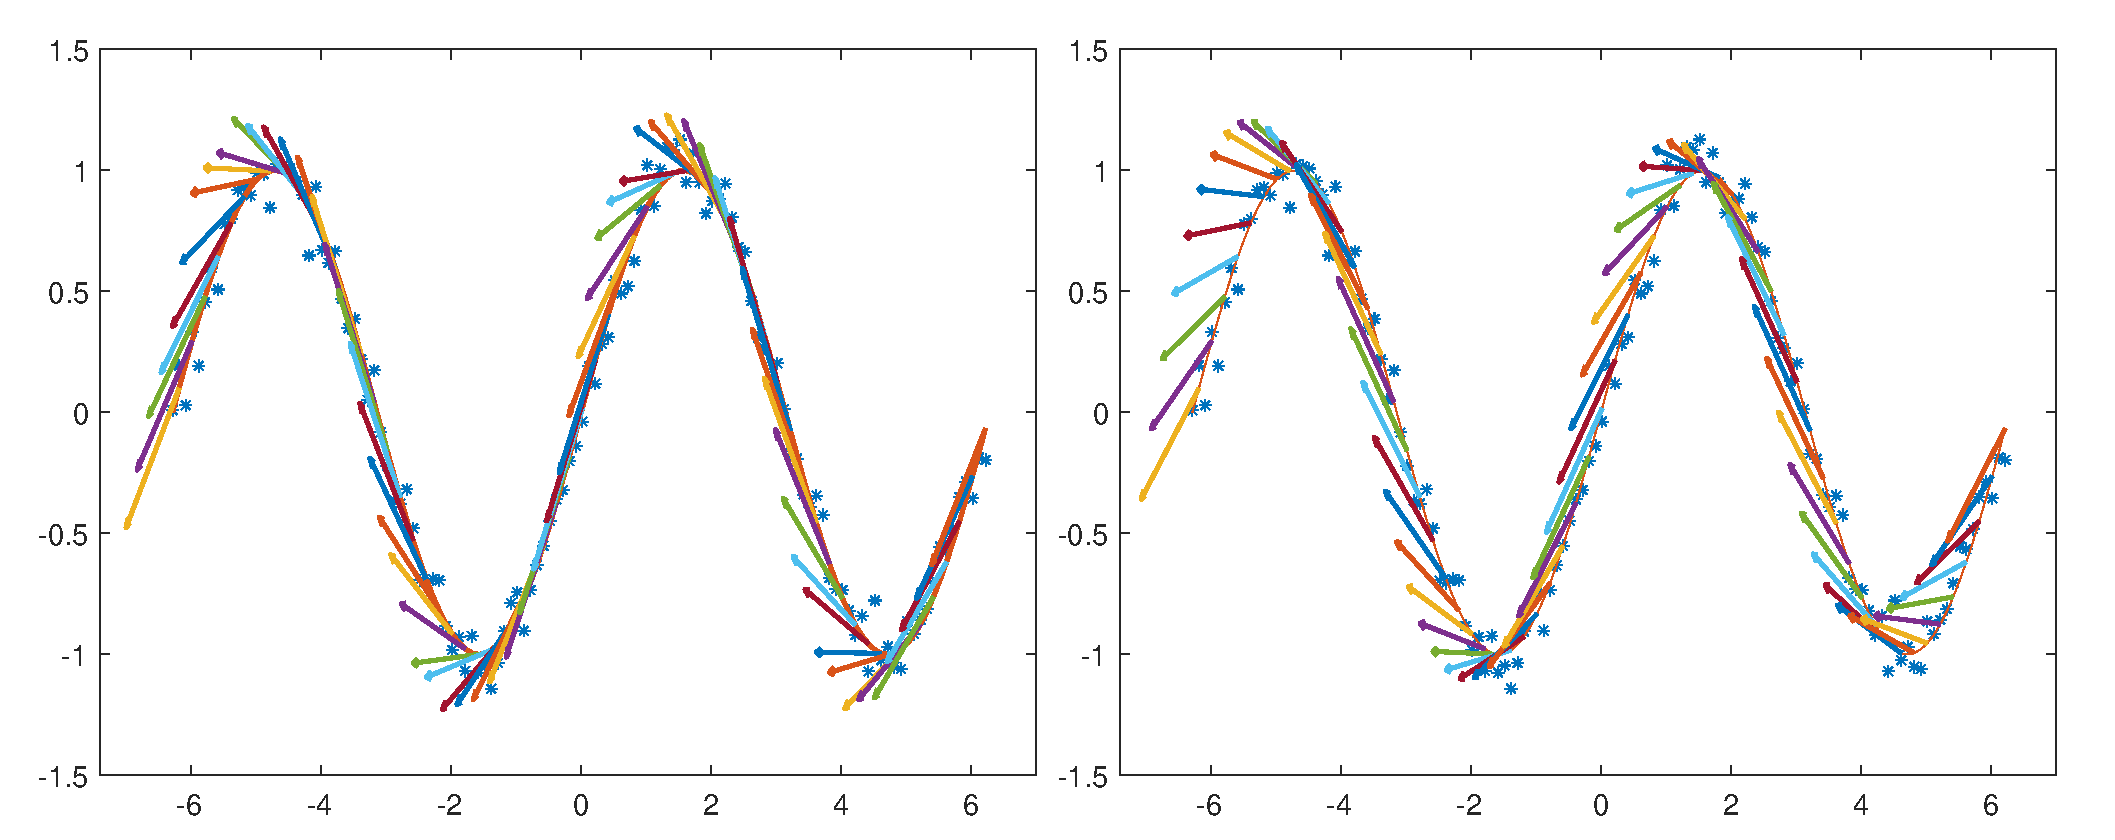
\includegraphics[width=\linewidth]{field_demo.eps} 
   \caption{Illustration of the vector field. Left: using partial nearest samples Right: using all samples}
   \label{fig:example}
\end{figure}

The effect of improving the quality of $C(x)$ by neglecting samples with a large scale can be seen in the vector field in the above figure. The vector field is constructed from the dominant eigenvector of the weighted covariance matrix $C(x)$. In the left diagram, the set $S$ is the k-nearest neighborhood of $x$, and in the right diagram the set $S$ represents all the samples. From the figure, we know that by selecting partial nearest samples we can get a weighted covariance matrix to approximate the vector field better.

Based on the above intuition, we show that constructing the KDE function by neglecting the far-away samples will help to reduce the point-wise bias of the derivatives. The reduced-bias phenomenon will further lead us to a ridge that is more 'close' than that by using all the samples.
 \subsection{Main Contributions}
Our contributions consist mainly of the following:
\begin{itemize}
\item[1.] We propose to use the partial nearest samples to construct a local KDE function, and use it to construct the ridge-estimator function. The proposed LKDE function can obtain a ridge that is more close to the original manifold, as the numerical experiment demonstrated.
\item[2.] We provide the theoretical result of the component-wise bias and variance corresponding to the LKDE function and prove that, under mild conditions, the local kernel function can indeed reduce the derivatives' bias more effectively than the KDE function.
\item[3.] By building the connection Hessian with the semi-positive definite covariance matrix, we show the necessity of rank-one modification to obtain a stable tangent space estimator.
%\item[1.] We build up the connection of the two common ways (Kernel Density Estimation and Tangent Space Estimation) to define the fitted manifold. 
%\item[2.] By analyzing the eigen-space of the Hessian matrix $H(x)$ of the Kernel Density Estimation function, we show that the normal space is not always generated by the principle eigenvectors of $H(x)$. To solve this problem, we split the $H(x)$ into two parts, $A(x)$ and $B(x)$. By estimating the normal space from $B(x)$, we can get a stable estimate of the normal space. The numerical experiment also demonstrates the effectiveness of our method.
%\item[3.] Our method not only can move an outlier $x_i$ onto the manifold, but also restricts the path of the convergence to be in the normal space of the interested targeting point $c(x)$.
%\item[4.] We also provide a faster algorithm to cope with the vanishing-gradient phenomenon for the kernel density function.
\end{itemize}
Finally, we provide numerical examples to show the effectiveness of our strategy, and also show that the vector field corresponding to our method is smoother and more appropriate for the ridge-estimation problem.
\subsection{Notations}
The most frequently used symbols and notations are listed in the table \ref{symbols}.

\begin{table}[h]\label{symbols}
\caption{Symbols and Notations}
\resizebox{12cm}{!}{
\begin{tabular}{c|c}\hline
Symbols & Meaning and Explaination\\\hline
$d$,$D$ & The dimension of the manifold and the dimension of the ambient space\\
${\rm E},{\rm Var}$ & The expectation and the variance operator\\
$\mathcal M,\hat{\mathcal G}$ & The hidden manifold and the estimated discrete data set satisfying the ridge definition\\ 
$\mathcal M_{\hat{G}}$ & The projection of the discrete set $\hat{\mathcal G}$ onto $\mathcal M$\\
$p_n(x),g_n(x),H(x)$& The KDE, its gradient, and the Hessian Matrix\\
$p_{r,h}(x),g_{r,h}(x),H_{r,h}(x)$& The local KDE, its gradient, and the Hessian Matrix\\
 $\Pi,\Pi^c$ & The projection onto the top $d$ eigenvectors and its orthogonal complement\\
 $f$ & The nonlinear increasing, nonnegative, and concave function\\ 
 $J(x)$ & The semi-positive definite matrix, which is a key component of the Hessian\\ 
 $\Pi_H$ & The projection matrix constructed by the top $d$ eigenvectors of $H$ \\ \hline 
\end{tabular}}
\end{table}


\subsection{Related Work}
\cite{ozertem2011locally} proposed a KDE-based subspace mean-shift algorithm (SCMS) to find the principal curve projection where the kernel density function is defined as a data-related covariance sum of kernel functions $\hat{p}(x) = (1/N)\sum_i G_{\Sigma_i}(x -x_i) $. By setting $\nabla \hat{p}(x) = 0$, we can obtain the mean-shift iteration: 
\[
x\leftarrow m(x) = (\sum_i c_i \Sigma_i^{-1} )^{-1} \sum_i c_i \Sigma_i^{-1}x_i.
\]
Directly applying the mean-shift algorithm will make $x$ converge to the local maximum of $p(x)$, which we call a mode. By restricting $x$ to converge to the $d$ dimension ridge defined by $p(x)$, the subspace-constrained mean-shift iteration \cite{ozertem2011locally} is given as
\[
x\leftarrow m(x) =V_{\perp} V_{\perp}^T (\sum_i c_i \Sigma_i^{-1} )^{-1} \sum_i c_i \Sigma_i^{-1}x_i,
\]
where $V_{\perp}$ is the eigenvectors corresponding to the D-d largest eigenvectors of the Hessian matrix $\Sigma^{-1} = -\hat{p}^{-1}(x)\hat{H}(x)+\hat{p}^{-2}(x)\hat{g}(x)\hat{g}(x)^T$, where $\hat{H}(x), \hat{g}(x)$ are the Hessian and gradient of $\hat{p}(x)$.

\cite{myhre2016manifold} proposed to use the spectral decomposition of the Hessian matrix $H(x) = Q(x)\Lambda(x)Q(x)^T$, and, furthermore, decompose $Q(x)$ into $Q(x)=[Q_\perp(x), Q_{\|}(x)]$, where $Q_\perp(x)$ is the eigenvectors corresponding to the $d$ largest eigenvalues of $H(x)$. Then, projecting points onto a density ridge can be rendered as the following initial value problem:
\[
\frac{d x(t)}{dt} = Q_{\perp}(x(t)) Q^T_{\perp}(x(t)) g(x(t)), \quad x(0) = x_0,
\]
where $g(x(t))$ is the gradient of $P(x)$ at $x(t)$.

\cite{mohammed2017manifold} also performed the gradient-ascent algorithm in the direction of $VV^Tg$, with $V$ consisting of the eigenvectors corresponding to the D-d largest eigenvalues, and $g$ being the gradient of the approximate squared-distance function (asdf). The asdf is defined as a minus $\log$ transform of density function $p(x)$ or a weighted summation of squared distance for each cylinder.

Besides being defined with a kernel density function, the manifold can also be defined with the zero points $\{x| F(x)={\bf 0}\}$ of a vector-valued function $F(x): R^D \rightarrow R^D$.  Suppose the observation data points $\{x_i, i=1:N\}$ are generated from the ideal low-dimensional manifold disturbed by some noise $x_i = x^*_i + \xi_i$, where $p^*$ is sampled from an ideal lower-dimension manifold and $\xi_i$ is the noise abeying some distribution. These methods, such as \cite{fefferman2018fitting, mohammed2017manifold, yao2019manifold}, normally need to estimate the local tangent space of the points residing in the neighborhood of the interested point $x$. The vector-valued function $F(x)$ is defined differently in works with different initiatives. For example,  \cite{fefferman2018fitting} define the function $F(x)$ as
\[
F(x)= \Pi_x \sum_i \alpha_i(x) \Pi^i(x - x_i).
\]
Furthermore, Yao and Xia simplify the two-step projection format into $F(x)= \Pi_x \sum_i \alpha_i(x) (x - x_i)$ by neglecting the inner projection $\Pi^i$. They also show the simplified version, which can also achieve good performance by \cite{yao2019manifold}.

Chen provides some theoretical results, such as the smoothness theorem, stability theorem, and convergence property of the gradient flow on the solution manifold, in \cite{chen2020solution}. The solution manifold is defined as a set of points satisfying the abstract form $\{x| \Psi(x) = 0\}$.

\section{Manifold Estimation}

We adopt the classical kernel density estimation approach to handle our manifold-fitting problem, as the majority of previous works do. From the kernel density perspective, the manifold can be viewed as points that satisfy some specific ridge conditions of the estimated density function.
\subsection{Ridge Definition}
There are two main definitions of a ridge, which involve describing the eigenspace of the Hessian and the gradient.
\begin{definition}
A point $x$ is on the d-dimensional ridge R of its probability density function when the gradient $g(x)$ is orthogonal to at least D-d eigenvectors of $H(x)$ and the corresponding D-d eigenvalues are negative. \cite{ozertem2011locally}
\end{definition}
This definition only gives us a condition to test whether a point $x$ lies on the d-dimensional ridge. However, given any $\hat{x}$, it does not tell us how to pull it onto the d-dimensional ridge. There are D-d eigenvectors of $H(x)$ that are orthogonal to the gradient $g(x)$, but it does not tell us the eigenvalues of $H(x)$ to which the eigenvectors correspond.

In some other works, such as \cite{genovese2014nonparametric}, the ridge is defined more concretely by restriction of the specific eigenvectors. Given any density function $p(x)$, we can define the ridge as the subset of the domain that satisfies
\begin{equation}\label{ridgeDF}
R = \{x| \Pi^{\perp}(H(x)) g(x) = 0, \lambda_{d+1}(H(x))<0\},
\end{equation}
where $H(x)$ is the Hessian matrix of $p(x)$, $g(x)$ is the gradient, and $\Pi^{\perp}$ is the projection onto the eigenspace spanned by the D-d smallest eigenvalues. Likewise, from the predefined functions $p_n(x)$ and $p_{r, h}(x)$, we can also have the ridges $R_n$ and $R_{r, h}$ corresponding to the density functions $p_n(x)$ and $p_{r,h}(x)$, respectively.

When $H(x)$ has exactly D-d negative eigenvalues, these two definitions have no practical differences. However, when $H(x)$ has more than D-d negative eigenvalues, then, from Definition 1, we have multiple choices to build the space to satisfy the ridge definition. Under this condition, the ridge in \eqref{ridgeDF} is only one choice, such that the ridge corresponding to definition \eqref{ridgeDF} is a subset of Definition 1.

From the definition, we can see that the ridge set $R$ is closely related to the Hessian $H(x)$ and the gradient $g(x)$. In the following section, we will show the connection between the distance between the ridges and the bias of the Hessian and gradient. 



\subsection{Ridge Estimation and Error Measurement}
In real cases, we use the ridge $R$ as an approximation of the unknown manifold $\mathcal M$ numerically. However, the definition of a ridge in \eqref{ridgeDF} is excessively descriptive and obscure. We can only judge whether a point resides on the ridge, but the definition provides an explicit continuous function to describe the ridge. In practice, we often randomly generate a mesh of initial points and use an algorithm to move the points onto the ridge by satisfying the ridge definition. As a result, what we finally obtain is a set of modified samples, $\hat{\mathcal G}$, satisfying the ridge definition. Furthermore, we can specify the estimator $\hat{\cal G}$ in \eqref{Estimator} as
\[
\hat{\mathcal G} = {\rm Algorithm}(\{x_1,...,x_n\},  R(\hat{p}_h(x)))
\]
which stands for $\hat{\mathcal G}$ relies on the initial random points $\{x_i\}$, the ridge $R$ derived from the the empirical density function $\hat{p}_h(x)$ and also the algorithm-computational factors which determine how we process our data $\{x_i\}$ by moving them onto the defined ridge.
\begin{figure}[htbp] %  figure placement: here, top, bottom, or page
   \centering
   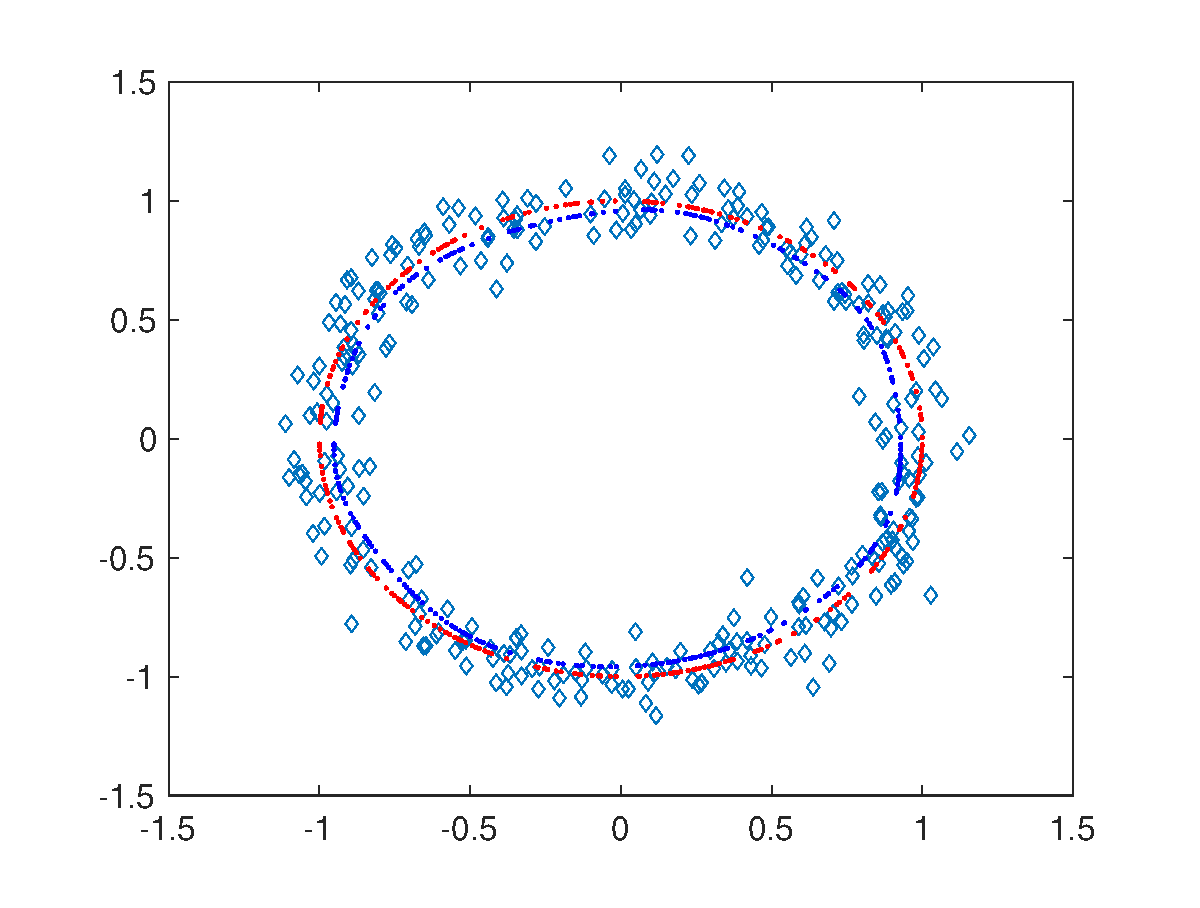
\includegraphics[width=3.5in]{introduction_demo.eps} 
   \caption{Illustration of the $\hat{\mathcal G},\mathcal M, \mathcal M_{\hat{\mathcal G}}$ and the Hausdorff and Average Margin by a toy circle example; The blue diamond markers stand for the observation points. The blue dots stand for the computed points which satisfy the ridge condition, i.e, $\hat{\mathcal G}$. The red dots stands for the projection of $\hat{\mathcal G}$ onto $\mathcal M$, which we denoted as $\cal M_{\hat{G}}$.  }
   \label{fig:example}
\end{figure}

Because $\hat{\mathcal G}$ is a discrete set and $\mathcal M$ is supposed to be continuous and smooth, the two sets have different cardinalities. Consider an extreme case where $\hat{\mathcal G}$ is a discrete subset of $\mathcal M$. Obviously, the largest distance from $\mathcal M$ to $\hat{\mathcal G}$ is $\sup_{x\in \mathcal M}\inf_{y\in\hat{\mathcal G}} \|x-y\|_2$, which is largely affected by the samples' distribution in $\hat{\mathcal G}$.

To diminish the random factor in the distance measurement between $\hat{\mathcal G}$ and $\mathcal M$, we extract a subset from $\mathcal M$ as ${\mathcal M}_{\hat{\mathcal G}}=\pi_{\mathcal M}(\hat{\mathcal G})$ and consider the Hausdorff distance between. Since the projection $\pi_{\mathcal M}(\hat{\mathcal G})$ from $\hat{\mathcal G}$ to $\mathcal M_{\hat{G}}$ is onto, the Hausdorff distance equals the quasi-Hausdorff distance
\begin{equation}\label{Hausd}
{\rm Haus}({\hat{\mathcal G}}, {\mathcal M}_{\hat{\mathcal G}}) = \max_{x\in \hat{\mathcal G}} \min_{y\in {\mathcal M}_{\hat{\mathcal G}}}\|x-y\|_2.
\end{equation}
The Hausdorff distance is the largest margin between $\hat{\mathcal G}$ and ${\mathcal M}_{\hat{\mathcal G}}$. The largest margin is dominated by only one point in $\hat{\mathcal G}$, which cannot reflect the overall margin level. So we also consider the average margin, defined as
\begin{equation}\label{margin}
{\rm Margin}({\hat{\mathcal G}, {\mathcal M}_{\hat{\mathcal G}}}) = \frac{1}{|\hat{\mathcal G}|} \sum_{x_k\in \hat{\mathcal G}} \min_{y\in {\mathcal M}_{\hat{\mathcal G}}}\|x_k-y\|_2,
\end{equation}
where $|\cal \hat{G}|$ represents the number of samples in $\cal \hat{G}$.
The distances, no matter Hausdorff or average margin, are complicated to bound or optimize directly. We need the following assumption:
\begin{assumption}\label{Data_assumption}
 Assume the points on $\hat{\cal G}, \cal M_{\hat{G}}$ satisfy the ridge definition corresponding two density functions $\hat{p}(x), p(x)$ respectively. 
\end{assumption}
\begin{remark}
This assumption can be achieved by selecting the appropriate forms of $\hat{p}(x), p(x)$. In this way, we can connect the distance between two points on $\hat G, \cal M_{\hat{G}}$ with the analytic quantity of the density functions $\hat{p}(x), p(x)$. For completeness, we give the proof of the connection between the ridge and the derivatives. 
\end{remark}
\begin{lemma}{ 
The pairwise distance between two data sets $\hat{G}$ and $\cal M_{\hat{G}}$ is of order $O(\|\hat{H}(x)-H(x)\|_F+\|\hat{g}(x)-g(x)\|_2)$, where $\hat{H}(x), \hat{g}(x)$ are the Hessian and gradient of some estimated density function $\hat{p}(x)$; $H(x)$ and $g(x)$ are the Hessian and gradient of the density function of $p(x)$.
%For any two ridges $R, \hat{R}$ defined by $R = \{x| \Pi_{H}(x)g(x) = 0\}$,$\hat{R} = \{x| \Pi_{\hat{H}}(x))\hat{g}(x) = 0\}$, 
 %$d(x, \hat{R}) = O(\|\hat{H}(x)-H(x)\|_F+\|\hat{g}(x)-g(x)\|_2)$
 }\label{margin}
\end{lemma}
The proof of Lemma \ref{margin} can be seen in appendix \ref{Ridge Derivative Lemma}.
\begin{remark}
Lemma \ref{margin} builds the bridge between the geometric quantities and the analytic differential quantities. By this lemma, we can easily convert the problem of searching a 'closer 'ridge to the problem of searching a 'better' approximation of the Hessian and gradient. This conversion can make our work more concrete and tractable.
\end{remark}

By the assumption \ref{Data_assumption} and Lemma \ref{margin}, we have, for any $x_k\in \hat{\mathcal G}$, there is $y_k\in {\mathcal M_{\hat{G}}}$ which is the end point of $\gamma(t)$ starting from $x_k$. Meanwhile, both of $x_k$ and $y_k$ satisfy the ridge definition in \eqref{ridgeDF}. 
Thus, we know that 
\begin{equation}\label{pointwise-bound}
\min_{y\in {\mathcal M}_{\hat{\mathcal G}}}\|x_k-y\|_2 \leq \|x_k-y_k\|_2 = O (\|\hat{H}(x_k)-H(x_k)\|_F+\|\hat{g}(x_k)-g(x_k)\|_2  ).
\end{equation}
From \eqref{Hausd}, by maximizing the distance with respect to $x_k\in 
\hat{\cal G}$ in \eqref{pointwise-bound}, we know that ${\rm Haus}({\mathcal {\hat{G}}}, {\mathcal M}_{\mathcal {\hat{G}}})$ yields a uniform upper bound by the sup norm in the right side:
\begin{equation}\label{Hausmargin}
{\rm Haus}({\hat{\mathcal G}}, {\mathcal M}_{\hat{\mathcal G}}) = O (\sup_x( \|\hat{H}(x)-H(x)\|_F+\|\hat{g}(x)-g(x)\|_2 ) ).
\end{equation}
\begin{remark}
When we approximate $\hat{p}(x), \hat{g}(x), \hat{H}(x)$ by the kernel density function as $\hat{p}_n(x), \hat{g}_n(x), \hat{H}_n(x)$, where the subscript $n$ means the functions are related with the samples and the sample size $n$. The pairwise error yield a result as
\[
\begin{aligned}
& ( |\hat{g}_n(x)-g(x)|)_i = O(h^2) + O_p((\frac{1}{{{n h^{D+2}}}})^{1/2}),\\
& ( | \hat{H}_n(x)-H(x)| )_{ij} = O(h^2) + O_p((\frac{1}{{{n h^{D+4}}}})^{1/2}).
\end{aligned}
\]
The empirical process theory gives the uniform error as
\[
\begin{aligned}
& \sup_x( |\hat{g}_n(x)-g(x)|)_i = O(h^2) + O_p((\frac{\log n}{{{n h^{D+2}}}})^{1/2}),\\
& \sup_x( |\hat{H}_n(x)-H(x)| )_{ij} = O(h^2) + O_p((\frac{\log n}{{{n h^{D+4}}}})^{1/2}).
\end{aligned}
\]
The error rate for the pairwise and uniform differs only in the stochastic term with a scale of $\sqrt{\log n}$. \cite{chen2017tutorial,JMLR:v17:ariascastro16a, genovese2014nonparametric}.
\end{remark}
%From \eqref{Hausmargin}, we can conclude that the Hausdorff distance of ${\mathcal G}$ and ${\mathcal M}_{\mathcal G}$ is controlled by the uniform approximation error of the Hessian and gradient, as $\sup_x( \|H_n(x)-H(x)\|_2+\|g_n(x)-g(x)\|_2$. The uniform derivatives rate is proved to be $L_{\infty}$, and the norm as , where the difference is the result of introducing $\log n$. This result is shown in \cite{JMLR:v17:ariascastro16a, genovese2014nonparametric}.
%Clearly, the Hausdorff distance between is the largest gap. As shown in \cite{genovese2014nonparametric}, the Hausdorff distance between the manifold and the ridge yields a uniform bound 
%${\rm Haus}({\mathcal G}, {\mathcal M}_{\mathcal G}) = O(h^2) + O_p((\frac{\log n}{{{n h^{d+4}}}})^{1/2})$. When $h={(\frac{\log n}{n}})^{1/(d+8)}$, the optimal minimum achieved is $O_p((\frac{\log n}{n})^{2/(d+8)})$. This optimum is the estimated convergent speed for the Hausdorff distance with the process of increasing the sample size $n$ and simultaneously decreasing $h$. However, in this paper, we mainly focus on how to get a closer ridge under the current observations, i.e. the number of samples is fixed.

Unlike the upper bound of the Hausdorff distance shown in \eqref{Hausmargin}, the average margin ${\rm Margin}(\hat {\mathcal G}, M_{\hat{G}})$ is closely related to the point-wise approximation error of $O (\|\hat{H}(x)-H(x)\|_F+\|\hat{g}(x)-g(x)\|_2)$. To reduce the average margin, we should focus on finding a new density function to improve the point-wise error with respect to the gradient and Hessian, and hope that this improvement of the error will lead to good performance of the estimated ridge.

As far as we know, the most widely used nonparametric approach to approximate $p(x)$ is the kernel density estimation (KDE) method. Next, we will review the classical KDE approach to approximate a density function, and derive the details of the corresponding derivatives' approximation error.
\subsection{Derivatives for KDE}
%Suppose we have multidimensional samples $\{x_k, x_k \in {\mathbb R}^D\}$ from a distribution $p(x)$. Then, we can build a kernel density function to estimate $p(x)$ using the kernel's summation from all the samples, as follows:
%\begin{equation}\label{KDE}
%p_n(x) = \frac{1}{n h^D} \sum_k K(\frac{x-x_k}{h}).
%\end{equation}
%The kernel $K(u)$ is supposed to be positive and differentiable at least with an order 2 and satisfies
%\[
%\int K(u) du = 1, \int u K(u) du = 0, \int \|u\|_2^2 K(u) du >0.
%\]
As the derivatives' bias generated from the kernel density function is highly related to the distance between the ridges constructed by $p(x)$ and $\hat{p}_n(x)$, respectively. We introduce the bias of the first-order and second-order derivative when using the kernel density function to approximate the real density function.
\subsubsection{Derivative Bias}
To derive the bias of the first-order and second-order derivative, we need to repeatedly implement the integration by substitution method on multiple-variables function. For the sake of completeness, we first recall some results for the bias and variance with respect to the derivatives. Subsequently, we show that the LKDE can improve the bias and variance results more than the classical KDE.

\begin{theorem}
The bias of the first order and second order of the KDE is 
\begin{equation*}\label{BiasResult}
|{\rm E}(\partial_{x_s}  \hat{p}_n(x)) - \partial_{x_s}p(x)|  \leq \frac{\lambda_s(x)}{2} h^2 \int \|u\|_2^2 K(u) du+o(h^2),
\end{equation*}
\begin{equation*}\label{order2}
|{\rm E}( \partial_{x_s} \partial_{x_t}  \hat{p}_n(x)) -  \partial_{x_s} \partial_{x_t} p(x)| \leq \frac{\lambda_{st}(x)}{2} h^2 \int \|u\|_2^2 K(u) du+o(h^2).
\end{equation*}
where $\lambda_s(x)$ is the largest eigenvalue of the Hessian matrix $H(\partial_{x_s}p(x))$ and $\lambda_{st}(x)$ is the largest eigenvalue of the matrix $M_{st}$ whose $i,j$-th element is $\frac{\partial^4}{\partial x_s\partial x_t \partial x_i \partial x_j} p(x)$, i.e., $\lambda_{st}(x)= \max_k \lambda_k( M_{st}(x))$.
\end{theorem}
We place the details of the procedure for proof in appendix \ref{bias_proof}.
\begin{remark}
It should be noted that in \eqref{BiasResult} and \eqref{order2} the square term $h^2$ originates from the fact that the positive kernel is of order 2, which is fixed and cannot be improved. However, we can make $\int \|u\|_2^2 K(u)du$ much smaller by making a small modification- {\it truncating the kernel}- as discussed below.
\end{remark}
\subsubsection{Derivative Variance}
After we get the bias of the derivatives, to get a better understanding of the stochastic property of the derivatives, we should also consider the variance. In this section, we give the variance result of the first and second derivatives of the KDE under the i.i.d. samples assumption. 
\begin{theorem}
The variance of the first and second order derivatives for KDE has a bound as 
\begin{equation*}\label{VarResult}
{\rm E} |\partial_{x_s} \hat{p}_n(x)-{\rm E}(\partial_{x_s} p_n(x))| \leq \sqrt{\frac{p(x)\int M^2(u)du}{n h^{D+2}}},
\end{equation*}
\begin{equation*}\label{VarResult2}
{\rm E} | \partial_{x_s}\partial_{x_t} \hat{p}_n(x) -\partial_{x_s}\partial_{x_t} p(x)| \leq \sqrt{\frac{p(x)\int N^2(u)du}{nh^{D+4}}}.
\end{equation*}
where $M(u) = \partial_{u_s}K(u)$ and $N(u) = \partial_{u_t}\partial_{u_s}K(u)$, respectively.
\end{theorem}
We place the details of the procedure for proof in appendix \ref{variance_proof}.

\subsubsection{Optimal-Parameter Dilemma}
The bandwidth parameter $h$ controls the smoothness of the density function and its derivatives. We can derive the best possible $h$ to obtain the best approximation error for the kernel density function. However, we cannot select a single optimum $h$ to be the optimum solution for the multiple objectives, such as the first-order and second-order derivatives.

Using the triangle inequality of absolute function, we derive the upper bound for the $|\partial_{x_s} \hat{p}_n(x) - \partial_{x_s} p(x)|$ by
\[
|\partial_{x_s} \hat{p}_n(x) - \partial_{x_s} p(x)|\leq |{\rm E}(\partial_{x_s}  \hat{p}_n(x)) - \partial_{x_s}p(x)|+ |{\rm E}  (\partial_{x_s} \hat{p}_n(x)) -\partial_{x_s}\hat{p}_n(x)| .
\]
The first term $|{\rm E}(\partial_{x_s}  \hat{p}_n(x)) - \partial_{x_s}p(x)|$ is deterministic and the second term $|{\rm E}  (\partial_{x_s} \hat{p}_n(x)) -\partial_{x_s}\hat{p}_n(x)|$ is a random variable. From \eqref{BiasResult} and \eqref{VarResult}, we know the upper bound of $|\partial_{x_s} \hat{p}_n(x) - \partial_{x_s} p(x)| $ is
\[
|\partial_{x_s} \hat{p}_n(x) - \partial_{x_s} p(x)| \leq  \frac{\lambda_s(x)}{2} h^2 \int \|u\|^2 K(u) du +O_p( \sqrt{\frac{p(x)\int M^2(u)du}{n h^{D+2}} } ).
\]
Obviously, for the first-order partial derivative, the optimum $h$ should minimize the objective $C_1(x)h^2+C_2(x)\frac{1}{\sqrt{n h^{D+2}}}$. Thus, $h = O({n^{-\frac{1}{D+6}}})$.
\[
|\partial_{x_s}\partial_{x_t} \hat{p}_n(x) - \partial_{x_s}\partial_{x_t} p(x)| \leq \frac{\lambda_{st}(x)}{2} h^2 \int \|u\|_2^2 K(u) du + O_p(\sqrt{\frac{p(x)\int N^2(u)du}{nh^{D+4}}}).
\]
In the same way, for the second-order partial derivative, the optimum $h$ should minimize the objective $C_3(x)h^2+C_4(x)\frac{1}{\sqrt{n h^{D+4}}}$ as well. Thus, $h = O(n^{-\frac{1}{D+8}})$. Obviously, we cannot minimize the first and second derivative approximations at the same time.

Next, we bring in another parameter $r$ to restrict our objective function such that we can construct the KDE by only using the samples with better quality in a surrounding neighborhood of $x$.
%\section{Locally Defined Kernel Density Estimation}
\subsection{Local Kernel Density Function}
In this paper, we consider a type of generalized, locally defined kernel $K_r (\frac{x-x_k}{h})$, controlled by two parameters $r$ and $h$, $h$ being the bandwidth that controls the distribution of each of the samples $x_k$ in a soft manner, and $r$ determining which partition of the samples should be used in our kernel density function.
\begin{equation}\label{GKDE}
\hat{p}_{r, h}(x) = \frac{1}{n h^D}\sum_k K(\frac{x-x_k}{h}) I(\|x -x_k\|\leq r).
\end{equation}
The necessity of bringing in the kernel with two parameters is a result of the fact that, in some cases, we will fall into the dilemma of having to use a large $h$ to get a smoother estimation while, at the same time, needing a smaller $h$ to keep a low bias for the estimated density function and even the derivatives.

It should be noted that in \eqref{GKDE} we consider only the samples in the ball with a radius of $r$; this can also be regarded as a truncated kernel function by defining
\begin{equation}\label{TK}
K_r(\frac{x-x_k}{h}) = K(\frac{x-x_k}{h}) I(\|x -x_k\|\leq r),
\end{equation}
as $K_r(\frac{x-x_k}{h})$ does not have a derivative at $\|x-x_k\|_2=r$. From \eqref{TK}, we also know that
\begin{equation}\label{DTK}
|\frac{\partial}{\partial x_i} K_r(\frac{x-x_k}{h}) | \leq |\frac{\partial}{\partial x_i} K(\frac{x-x_k}{h})|, \forall, \|x-x_k\|\leq r,
\end{equation}
letting $u = \frac{x-x_k}{h}$. Obviously, if $K(u)$ satisfies $\int K(u)du=1$, it is easy to renormalize $K_r(u)$ by a constant value $c>1$ such that
\[
\int c K_r (u) du =  c\int_{\|u\|\leq r/h} K(u) du= 1.
\]
When $K(u) = \exp(-\|u\|^2_2)$, the error for normalization will be a small amount:
\begin{equation}\label{Perror}
 \int_{\|u\|\leq r/h} K(u) du =1- O(\exp(-(r^2/h^2))).
\end{equation}
When $r$ is far bigger than $h$, the residue part $O(\exp(-(r^2/h^2)))$ will become ignorable. Later, we use this relation in our bias-analysis section.
\subsubsection{Parameter Setup}
For a density function defined on a manifold $\mathcal M$ that is embedded in $\mathbb{R}^d$, if the density function $p(x)$ is large at $x_0$, we assume the manifold is more complicated at $x_0$ as it has a smaller local reach. In such a case, we would prefer to construct our local kernel density function in a smaller neighbor ${\mathcal N}(x_0,r)$. Conversely, if the density $p(x)$ is small, to obtain a more accurate estimation from the data, we would prefer to concentrate on a relatively large area.

For a particular $x$ such that $p(x)$ is relatively large, there is a high probability of sample $x_i$ being generated around $x$, i.e. the sample density around $x$ is higher relative to other places.
%In this paper, we assume that the parameter $r$ is related to the current $x$, from the intuition that when $p(x)$ is large a small partition

We determine $r(x)$ from the accumulating density function $\phi(x,r)=C$ such that the following value $\phi(x,r) $ is a constant $C$. $\phi(x,r)$ is defined as
\[
\phi(x,r) = \int_{y\in {\mathcal D}_r(x)} p(y) dy \approx \frac{1}{n} \sum_k I(x_k\in {\mathcal D}_r(x)).
\]
On real computational occasions, $r$ can be chosen as the smallest radius such that the set $\{x_k| \|x-x_k\|\leq r\}$ contains exactly $m$ elements, where $m$ is a predefined parameter.
%\subsection{Bias and Variance of Derivative of  $p_{r,h}(x)$}

As with the bias for the derivative of $\hat{p}_n(x)$, we also have the bias for the derivative $\hat{p}_{r,h}(x)$. It is easy to show that, under some conditions, the bias of the derivatives of $\hat{p}_{r,h}(x)$ is less than that of $\hat{p}_n(x)$.
\subsubsection{Upper Bound of the Bias}
In the previous section, we derived the upper bound of the bias for the classical KDE function. Here, we present the bias result of our LKDE, and show that, under some mild conditions, the bias for the LKDE is smaller than that of KDE.

%\[
%|{\rm E}(\partial_{x_s}  p_n(x)) - \partial_{x_s}p(x)|  \leq \frac{\lambda_s(x)}{2} h^2 \int \|u\|^2 K(u) du+o(h^2)
%\]
\begin{lemma} For the LKDE, we have the bias relationship as
\begin{equation*}\label{order11}
\begin{aligned} 
|{\rm E}( \partial_{x_s}  \hat{p}_{r,h}(x)) - & \partial_{x_s } p(x)| \\
\leq & \frac{\lambda_s(x)}{2} h^2 \int_{\|u\|\leq r /h} \|u\|_2^2 K(u) du +  \int_{\|u\|\geq r/h} K(u) du |\partial_{x_s} p(x)|,\\
\end{aligned}
\end{equation*}
\begin{equation*}\label{order22}
\begin{aligned}
 |{\rm E} (\partial_{x_s} \partial_{x_t}   \hat{p}_{r, h}(x)) -  &\partial_{x_s} \partial_{x_t} p(x)| \\
\leq &\frac{\lambda_{st}(x)}{2} h^2 \int_{\|u\|\leq r /h} \|u\|_2^2 K(u) du +  \int_{\|u\|\geq r/h} K(u) du  |\partial_{x_s} \partial_{x_t} p(x)| .
\end{aligned}
\end{equation*}
\end{lemma}
The proof can be seen in appendix \ref{LKDE bias}. By bring in two parameters $\gamma,\mu_s(x)$ Lemma \ref{LKDE bias} can be further simplified as Theorem \ref{bias_theorem}.

\begin{theorem}\label{bias_theorem}
If $|\partial_{x_s} p(x)| \leq \gamma h^2 \lambda_s(x)$ and $|\partial_{x_s} \partial_{x_t} p(x)| \leq \gamma h^2 \lambda_{st}(x)$, there will be $0<\mu_s(x)<1,0<\mu_{st}(x)<1$ such that the bias of $\partial_ {x_s} \hat{p}_{r,h}(x)$ and $\partial_{x_s} \partial_{x_t}  \hat{p}_{r, h}(x)$ will satisfy both of the following inequalities:
\[
\begin{aligned}
&|{\rm E} (\partial_ {x_s} \hat{p}_{r,h}(x)) -\partial_{x_s} p(x)| \leq \mu_s(x)( \frac{ \lambda_s(x)}{2} h^2 \int \|u\|_2^2 K(u) du),\\
&|{\rm E} (\partial_{x_s} \partial_{x_t}  \hat{p}_{r, h}(x))-  \partial_{x_s} \partial_{x_t} p(x)| \leq  \mu_{st}(x) (\frac{\lambda_{st}(x)}{2} h^2 \int \|u\|_2^2 K(u) du).
\end{aligned}
\]
\end{theorem}
The proof of Theorem \ref{bias_theorem} can be seen in appendix \ref{Simplified Bias Result}.
\begin{remark}
From comparing the above results with \eqref{BiasResult} and \eqref{order2}, we can conclude that the bias for LKDE is reduced with a scale of $\mu_s(x)$ and $\mu_{st}(x)$. In the following section, we also determine that the derivative's variance of LKDE is also bounded by that of KDE. 
\end{remark}
\subsubsection{Variance Upper Bound}
Recall that the variance of the partial derivative is
\[
{{\rm Var}}(\partial_{x_s} \hat{p}_n(x)) \leq \frac{1}{n h^{D+2}}  (p(x) \int (\partial_{ u_s } K (u) )^2  du.
\] 
Here, we can show that the variance of the local KDE also has a similar upper bound to that of KDE.
\begin{theorem}{The variance of derivative of $p_{r,h}(x)$ is controlled by}
\[
{{\rm Var}}(\partial_{x_s} \hat{p}_{r,h}(x)) \leq \frac{1}{n h^{D+2}}  (p(x) \int (\partial_{ u_s } K (u) )^2   du + O(h)).
\]
\end{theorem}
The proof can be seen in appendix \ref{Derivatives' Variance for LKDE}. By combining the bias and variance, we have the overall approximation for LKDE as
\subsubsection{Overall Approximation Error for LKDE}
Using the above analysis and Chebyshev's inequality, we obtain the overall approximation error for LKDE satisfying
\begin{equation}\label{bias_result_final}
\begin{aligned}
 &|\partial_{x_s} \hat{p}_{r,h}(x)-\partial_{x_s} p(x)|\\
 \leq & |\partial_{x_s} p(x) - {\rm E} (\partial_{x_s}\hat{p}_{r,h}(x)) |+(|\partial_{x_s} \hat{p}_{r,h}(x) - {\rm E} (\partial_{x_s}\hat{p}_{r,h}(x)) | )\\
 \leq & \mu_s(x)( \frac{ \lambda_s(x)}{2} h^2 \int \|u\|_2^2 K(u) du) + O_p(\sqrt{\frac{1}{n h^{D+2}}  (p(x) \int (\partial_{ u_s } K (u) )^2   du})).
\end{aligned}
\end{equation}
Similarly, for the second order differential form, we have
\[
\begin{aligned}
 &|\partial_{x_{s}}\partial_{x_t} \hat{p}_{r,h}(x)-\partial_{x_{s}}\partial_{x_t} p(x)|\\
 \leq & |\partial_{x_{s}}\partial_{x_t} p(x) - {\rm E} (\partial_{x_{s}}\partial_{x_t} \hat{p}_{r,h}(x)) |+|\partial_{x_{s}}\partial_{x_t} \hat{p}_{r,h}(x) - {\rm E} (\partial_{x_s} \partial_{x_t} \hat{p}_{r,h}(x)) | \\
 \leq & \mu_{st}(x)( \frac{ \lambda_{st}(x)}{2} h^2 \int \|u\|_2^2 K(u) du) + O_p(\sqrt{\frac{1}{n h^{D+4}}  (p(x) \int (\partial_{ u_s }\partial_{u_t} K (u) )^2   du})).
\end{aligned}
\]
Based on the relatively smaller approximation error, we can expect the ridge obtained from LKDE to have a smaller distance from the underlying manifold. To derive a uniform bound for distance in pairwise point measurement, we denote $\mu$ which will be used in our final result
\[
\mu = \sup_x \max_{s, t}\max\{\mu_s(x), \mu_{st}(x)\}.
\]
By selecting the optimum $h$ in the estimation of gradient and Hessian, we can get the estimate of margin between $\hat{\cal G}$ and $\cal M_{\hat{\cal G}}$ as following. Firstly, we observe that only improving one term in \eqref{bias_result_final} can indeed improve the optimum function value.
\begin{theorem}\label{improve_lemma}
For two functions $\nu(h) = a_0 h^2 + a_1 \sqrt{\frac{1}{nh^{D+m}}}$ and $\nu_\mu (h) = \mu a_0 h^2 + a_1 \sqrt{\frac{1}{nh^{D+m}}}$ with $m=2,4,\mu\in(0,1)$. Then, the optimal minimums of them have a relationship:  $\min_h \nu_\mu (h) = \mu^{\frac{D+2}{D+6}}\min_h \nu(h)$
\end{theorem} 
\begin{remark}
From theorem \ref{improve_lemma}, we know that by reducing the bias with a scalar of $\mu$, we will have the optimal minimum solution reduced with a scalar of $\mu^{\frac{D+m}{D+m+4}}$.  Noting that, with the increasing of the dimension $D$, we will obtain a smaller $\mu^{\frac{D+m}{D+m+4}}$. Theorem \ref{improve_lemma} justifies we can improve the ridges' between distance by reducing the derivatives' bias corresponding to the density function. Similarly, we also place the details in the appendix \ref{mimimum_proof}.
\end{remark}
%\begin{lemma}\label{improve_lemma}
%For a function $f(h) = a_0 h^2 + a_1 \sqrt{\frac{1}{nh^{D+4}}}$, the minimum is achieved at $h^* = \arg\min_h f(h) = (\frac{a_1^2}{n a_0^2})^{\frac{1}{D+8}}$, with the value
%\[
%f(h^*) = 2(\frac{a_1^2 a_0^{\frac{D+4}{2}}}{n})^{\frac{2}{D+8}}=2 a_0^{\frac{D+4}{D+8}} a_1^{\frac{1}{D+8}} {({\frac{1}{n}})}^{\frac{2}{D+8}}.
%\]
%Consider another function 
%\begin{equation}\label{f_mu}
%f_\mu (h) = \mu a_0 h^2 + a_1 \sqrt{\frac{1}{nh^{D+4}}}.
%\end{equation}
%where in \eqref{f_mu} we replace $a_0$ with $\mu a_0$ by multipling it by $\mu \in (0,1)$, this will lead to a new minimum optimum point for $f_\mu(h)$
%\[
%h^{**} =\arg\min f_\mu( h)=(\frac{a_1^2}{n \mu^2 a_0^2})^{\frac{1}{D+8}}.
%\] 
%Substitute it into \eqref{f_mu}, it is obviously $f_\mu (h^{**}) = \mu^{\frac{D+4}{D+8}}f(h^*)$.
%\end{lemma}
From Theorem \ref{improve_lemma}, we know that by replacing the KDE with LKDE, we will get an optimal ridge with the average margin reduced by a scalar $\mu^{\frac{D+2}{D+6}}$, :
\begin{theorem}
\[
{\rm Margin}(\hat{\cal G}_{LKDE}, {\cal M}_{\hat{\cal G}_{LKDE}}) \leq \mu^{\frac{D+2}{D+6}} {\rm Margin}(\hat{\cal G}_{KDE}, {\cal M}_{\hat{\cal G}_{KDE}}).
\]
\end{theorem}
\begin{remark}
With the increasing of the dimension $D$, the scalar $\mu^{\frac{D+2}{D+6}}$ will become more and more smaller. This asymptotical behaviors show that with process of increasing of dimension, the effect of LKDE will become more and more apparent compared with KDE.
\end{remark}
  
In this section, we consider the advantage of the bias and variance for the locally defined kernel density function over those of the classical KDE. The results show that, we can indeed obtain a ridge closer than that obtained from the classical KDE method.

Next, instead of the analyzing the element-wise partial derivatives, in a higher perspective, we give the spectral property of $H(x) = \nabla\nabla \hat{p}_{r,h}(x)$ with the smoothly moving of $x$, and show the necessity of transformation with a concave function.

\section{Transformation of $\hat{p}_{r,h}(x)$}
In this section, we mainly concern the relationship of two ridge $R_{\hat{p}_{r,h}(x)}$ and $R_{f_{\hat{p}_{r,h}(x)}}$ which stand for the ridge derived from two function $\hat{p}_{r,h}(x)$ and  $f( \hat{p}_{r,h}(x))$, respectively. Here, we give a deep analysis on the effectiveness of nonlinear function $f$ acting on the density function $\hat{p}_{r,h}(x)$.

The transformation of the density function is a composite function $f$ acting on $\hat{p}_{r,h}(x)$ as $f( \hat{p}_{r,h}(x))$. Usually, $f$ is chosen to be a function that has a first- and second-order derivative satisfying $f'(x)>0$ and $f''(x)<0$. There are two main benefits of the transformation.

Since the transformation of $\hat{p}_{r,h}(x)$ corresponds to a rank-one modification to the Hessian matrix, the ridge generated after the transformation will leave out some singular points, compared with the ridge from before.

The eigenspace of the Hessian of $f( \hat{p}_{r,h}(x))$ becomes more stable and has an intuitive explanation as a tangent space. However, the eigenspace of the Hessian of $\hat{p}_{r,h}(x)$ is more complicated because of the perturbation effect of the scale of a rank-one matrix.
\subsection{The Weighted-Covariance Form}
When we use a radial basis kernel function $K(u) = \phi(-\|u\|_2^2)$, the Hessian matrix $\nabla\nabla \hat{p}_{r,h}(x)$ yields a simple form of a covariance matrix added by a scaling matrix:
\begin{equation}\label{HP}
H_{\hat{p}_{r,h}}(x) =\frac{4}{nh^4}\{ \sum_{k\in {\mathcal I}_r } \phi''(-\|\frac{x-x_k}{h}\|^2)(x-x_k) (x-x_k)^T -\frac{h^2}{2}\sum_{k\in {\mathcal I}_r} \phi'(-\|\frac{x-x_k}{h}\|_2^2)I\}.
\end{equation}
Obviously, the key component 
$
\psi(x) = \sum_{k\in {\mathcal I}_r } \phi''(-\|\frac{x-x_k}{h}\|^2)(x-x_k) (x-x_k)^T,
$ determines the spectral property of $H_p(x)$. For convenience, the normalized second derivative can be denoted by: 
\[
w_h(x, x_k) = \phi''(-\|\frac{x-x_k}{h}\|^2)/\sum_{k\in I_r}\phi''(-\|\frac{x-x_k}{h}\|^2) .
\]
Naturally, $\sum_{k \in {\mathcal I}_r} w_h(x, x_k) = 1$. With this notation, the semi-definite covariance matrix can be simplified as a weighted summation of a rank-one matrix by
\begin{equation}\label{Jx}
J(x) = \sum_{k\in {\mathcal I}_r } w_h(x, x_k)(x-x_k) (x-x_k)^T.
\end{equation}
It can be observed that the matrix field $J(x)$ is parameterized by $x$, and so the eigenspace corresponding to the largest $d$ eigenvalues are largely affected by $x$. Next, we express the locally weighted mean $c_r(x)$ as
 \[
 c_r(x) =  \sum_{k\in {\mathcal I}_r }w_h(x, x_k) x_k.
 \]
%We then analyze the behavior of the eigenspace of $\hat{H}(x)$ with the approaching process of $x$, from far away to ???.
%To simplify the analysis, we define the center of data $\{x_i, i=1:N\}$ and base the observation at $x$ on:
%\begin{equation}\label{c(x)}
%c(x) = \frac{1}{\sum_i w(x, x_i)} \sum_{i=1}w(x, x_i) x_i
%\end{equation}
%As the function $\exp(-d^2)$ decreases very fast as $d$ increases, $c(x)$ can be considered a weighted convex combination within a neighborhood ${\mathcal N}_x$ of $x$.
%
%As $x_i -x$ is the most basic component of $\hat{H}(x)$, we provide a deep analysis of the different components comprising $\hat{H}(x)$. First, we bring in the observation center $c(x)$ by
Note that, in a $r$-ball of $x$, ${\mathcal M} \cap B_x(r)$ is approximately a local, lower-dimensional affine space. As a result, the weighted mean $c_r(x)$ also resides approximately on the affine space.
Since $x_k -x = c_r(x) -x + (x_k - c_r(x))$, by substituting it into \eqref{Jx} we have:
\begin{equation}\label{hhat}
\small{
\begin{aligned}
J(x) = &\sum_{k\in {\mathcal I}_r} w_h(x, x_k) (c_r(x) - x)(c_r(x)-x)^T + \sum_{k\in {\mathcal I}_r} w_h(x, x_k) (x_k-c_r(x)) (x_k-c_r(x))^T\\
+&\sum_{k\in {\mathcal I}_r } w_h(x, x_k)\{(c_r(x)-x) (x_k-c_r(x))^T+ (x_k-c_r(x))(c_r(x)-x)^T\}.\\
\end{aligned}}
\end{equation}
Using the definition of $c_r(x)$, we can see that
\[
\sum_{k\in {\mathcal I}_r} w_h(x, x_k) (x_k -c_r(x)) = \sum_{k\in {\mathcal I}_r} w_h(x, x_k) x_k -\sum_{k\in {\mathcal I}_r} w_h(x, x_k) c_r(x) = 0.
\]
Thus, we only need to consider the remaining two parts of \eqref{hhat}:
%In this case, $\sum_{i=1}^N \|x_i-c\|_2$ will majorize $N\|c(x)-x\|_2$, and so, in the same way, we have
\begin{equation}\label{Hw}
J(x) = (c_r(x) - x)(c_r(x)-x)^T + \sum_{k\in I_r} w_h(x, x_k) (x_k-c_r(x)) (x_k-c_r(x))^T.
\end{equation}
%$c(x)-x$ lies approximately lies the normal space at $c(x)$ and $x_i -c(x)$ lies approximately in the tangent space of $c(x)$. To simplify our analysis, we make the following assumption.
From \eqref{Hw}, we can see that $J(x)$  mainly consists of the following three parts:
\begin{itemize}
\item The d-dimensional affine space $\mathcal H$, which can be approximated by the eigenspace of the samples in the $r$ neighborhood of $x$, i.e. $\{x_k, k\in {\mathcal I}_r\}$, and shifted such that $c_r(x)\in \mathcal H$.
\item The one-dimensional affine space $\mathcal F$ spanned by $c_r(x)-x$ and shifted such that $c_r(x)\in \mathcal F$, where $c_r(x)$ is a convex combination of $\{x_k, k\in {\mathcal I}_r\}$.
\item The small fraction of noise from the observation samples that resides in the D-d dimensional affine space ${\mathcal H}^\perp$.
\end{itemize}
Clearly, the eigenspace ${\mathcal V}_d$, spanned by eigenvectors corresponding to the top $d$ largest eigenvalues of $J(x)$, is largely affected by the scale of $c_r(x)-x$. When $c_r(x)-x$ is large, it will have a much larger influence on the space of ${\mathcal V}_d$, and vice versa.

\begin{figure} %  figure placement: here, top, bottom, or page
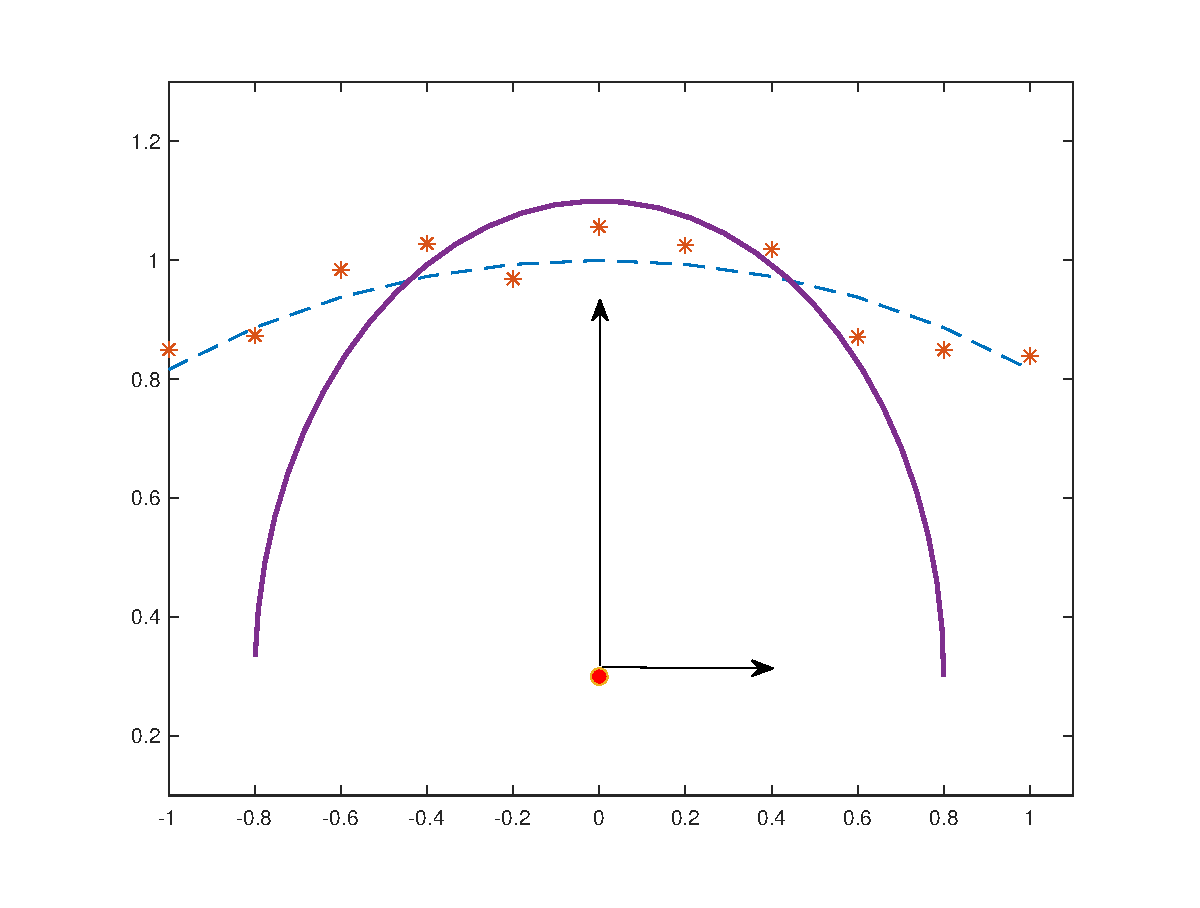
\includegraphics[width=0.32\linewidth]{../figures/demo1.eps} 
\hspace{-4mm}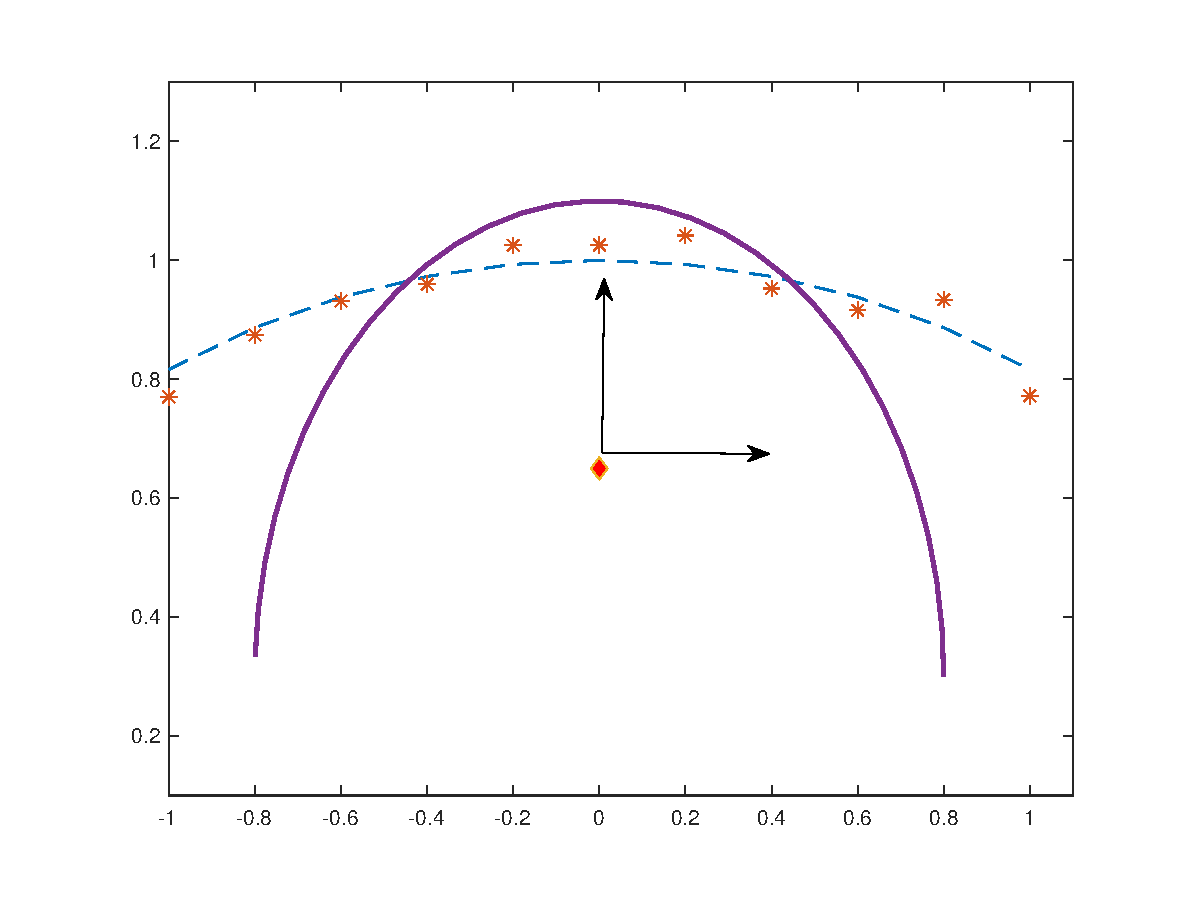
\includegraphics[width=0.32\linewidth]{../figures/demo2.eps} 
\hspace{-4mm}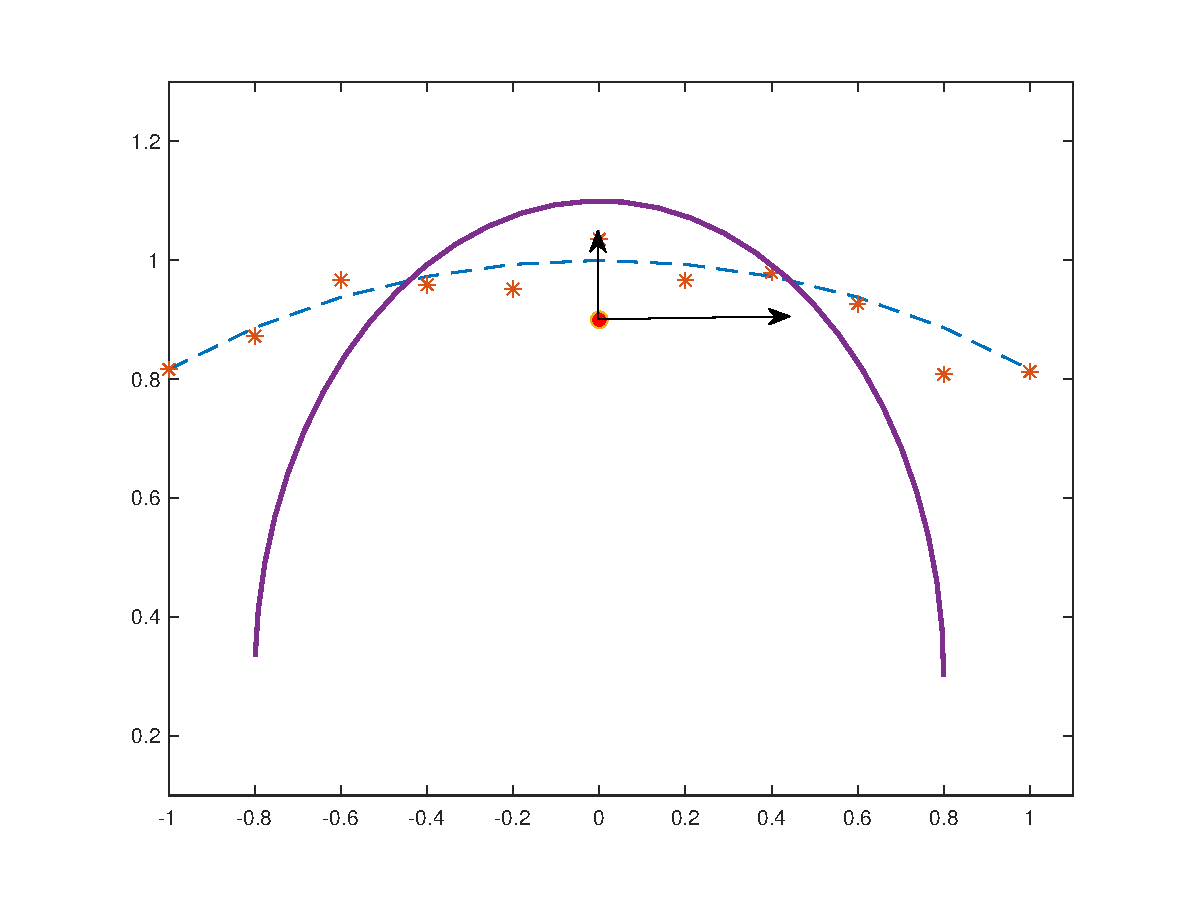
\includegraphics[width=0.32\linewidth]{../figures/demo3.eps} 
%\setcaptionwidth{6in}
\caption{The process of $J(x)$'s eigenspace's variation with $x$ approaching the manifold }
\label{Shifting Eigenvectors}
\end{figure}

Next, we give an example to illustrate the influence the scale of $c_r(x)-x$ on the eigenspace of $J(x)$ in Figure \ref{Shifting Eigenvectors}. The blue dash curve represents the hidden unknown manifold $\cal M$. The red star points stand for the observation points $x_i$ which is assumed sampled from the manifold $\cal M$ and disturbed by some noise. The middle red dot represents the location of $x$, which we want it to move towards the manifold from far away. The two orthogonal arrows represent the vectors $\{\lambda_k u_k, k=1,2\}$, where $\lambda_k$ and $u_k$ are the $k$-th eigenvalue and eigenvector of $J(x)$, respectively.

The left portion of the figure shows that, when $x$ is far away from the data points, the space spanned by the principal eigenvectors of $J(x)$ is approximately residing in the normal space of the manifold. With the process of $x$ coming near the ridge, we can see that the two eigenvalues of $J(x)$ will be equal, as shown in the middle portion of the figure. If $x$ continues approaching the ridge, we will see that the principal eigenvector will be parallel with the ridge.

The subspace-constrained shifting method requires $x$ to move in the normal space of the manifold to get the projection $x^*$ of $x$ onto the manifold. However, as $x$ is far away from the manifold and $x^*$ is unknown, to overcome this difficulty we can use the space spanned by the eigenvectors of $J(x)$, corresponding to some particular eigenvectors, as an approximation of the normal space at $x^*$. We show that this may cause some error because, as $x$ approaches the manifold, the magnitude of $\lambda_i/\lambda_{i+1}$ will change dramatically. Thus, picking the eigenvector corresponding to the largest eigenvalue may cause a sudden turn into the orthogonal direction. The unpredictable directional behavior of the principal eigenvector of $J(x)$ causes the searching lower-dimensional ridge algorithm to converge badly. Fortunately, this difficulty can be overcome by using a nonlinear transformation, as introduced in the next section. Through modification with a rank-one matrix, we can obtain a new $J(x)$ with a very stable eigenspace, i.e. the order of the first and second eigenvectors will not be reversed with the moving of $x$. %Below, we provide a simple two-dimensional example to illustrate this.
%The discussion can be split into three cases, depending on the relationship between $x$ and $\{x_i, i=1:N\}$.

\subsection{The Necessity of Transformation}
To simplify the analysis, we assume the orthogonality of $c_r(x)-x$ and the space spanned by the top $d$ eigenspace of $\sum_i w_h(x, x_i) (x_i-c_r(x)) (x_i-c_r(x))^T$.
\begin{assumption}
Assume the vector $c_r(x)-x$ is orthogonal to the subspace spanned by the eigenvectors corresponding to the top $d$ eigenvalues of the covariance matrix $C(c_r(x)) = \sum_i w_h(x, x_i) (x_i-c_r(x)) (x_i-c_r(x))^T$. 
\end{assumption}
If we denote the eigenvalue decomposition of $C(c_r(x))$ as 
\[
C(c_r(x)) = [ V_d, V_{D-d}] \Lambda [ V_d, V_{D-d}]^T,
\]
the principal space is spanned by the vectors consisting each of the columns of $V_d$. Here, $V_d$ relys on $x$ through $c_r(x)$, as a result, we denote $V_d$ as $V_d(c_r(x))$. Similarly, we have the space which is orthogonal to the principal space, which we denote as $V_{D-d}(c_r(x))$.

Based on the assumption, we can represent $c_r(x)-x$ and $\{x_i-c_r(x), i=1:n\}$ by the coordinates in their corresponding space as:
\begin{equation} \label{tangent2}
c_r(x) - x =  V_{D-d}(c_r(x)) \alpha(x); \quad x_i-c_r(x) = V_d(c_r(x))\alpha(x, x_i).
\end{equation}
Substitute \eqref{tangent2} into \eqref{Hw} and let
\begin{align*}
&A(x)= V_{D-d}(c_r(x)) \alpha(x) \alpha(x)^T V_{D-d}(c_r(x))^T,\\
&B(x)=\sum_i w(x, x_i) V_d(c_r(x)) \alpha(x, x_i)\alpha(x, x_i)^T V_d(c_r(x))^T ;
\end{align*}
We have
\[
J(x) =A(x) + B(x).
\]
In this case, we know ${\rm rank}(A(x))=1, {\rm rank} (B(x))=d$. For the rank-one matrix, we can get the eigenvalue  $\lambda(A(x))$ by normalizing $A(x)$. Note that
\[
A(x) = V_{D-d}(c_r(x))\frac{\alpha(x)}{\|\alpha(x)\|}  \|\alpha(x)\|_2^2 \frac{\alpha^T(x)}{\|\alpha(x)\|}  V^T_{D-d}(c_r(x))
\]
Thus, the eigenvalue value of $A(x)$ is $\|\alpha(x)\|_2^2$ and $V_{D-d}(c_r(x))\frac{\alpha(x)}{\|\alpha(x)\|}$ is a unitary vector in the space of $V_{D-d}(c_r(x))$. For simplicity, we denote 
\[
v(x) = V_{D-d}(c_r(x))\frac{\alpha(x)}{\|\alpha(x)\|},\quad
\Xi (x) = \sum_i w(x, x_i) \alpha(x, x_i)\alpha(x, x_i)^T,
\]
which will be used in our following discussion.
Similarly, the matrix $B(x)$ shares the same eigenvalues  with $\Xi (x)$, because the unitary transformation keep the singular values unchanged. 
%Let $A(x) =\sigma(A(x)) v(x)v(x)^T$, and 
Denote the eigenvalue decomposition of $\Xi (x)$ as  $\Xi(x) = \Theta(x) \Lambda(x) \Theta(x)^T$. Then, we have
\[
B(x) = V_d(c(x))\Theta(x) \Lambda(x)\Theta(x)^T V_d(c(x)).
\]
Note that $\Upsilon(x) = V_d(c(x))\Theta(x)$ is an orthonormal matrix satisfying 
$\Upsilon^T (x)\Upsilon(x)=I$. This can be divided into three cases based on the relationship between $\lambda(A(x))$ and $\lambda_{\min}(\Xi(x)), \lambda_{\max}(\Xi(x))$.
\subsubsection{Eigenspace Analysis}
Depending on the relation between the eigenvalue of $\lambda(A(x))$ and the eigenvalues of $\Xi(x)$, there are three different cases, as described in the next few paragraphs. Because the scale of the eigenvalue of $\lambda(A(x))$ can vary greatly, we cannot recover $V_d$ by just selecting the top $d$ eigenvectors of $J(x)$.

\subsubsection*{Case \romannumeral1: $\lambda(A(x))>\lambda_{\max} (\Xi(x))$}

This case corresponds to the leftmost diagram in {Figure \ref{Shifting Eigenvectors}}, where $x$ is far away from the data points. The covariance matrix $\sum_i w_h(x_i, x)(x_i-x)(x_i-x)^T$ will have large eigenvalues in the subspace of $V_{D-d}(c_r(x))$. Then, the eigenvector $V_{D-d}(c_r(x))\alpha(x)$ is the principal eigenvector, and we can distinguish it from the top eigenvector through eigenvalue decomposition.
Then, the eigen-decomposition of $J(x)$ is
\begin{equation}\label{SVD1}
J (x)= [v(x), \Upsilon(x)] 
\left[
\begin{array}{cc}
\lambda(A(x)) & \bf 0\\
\bf 0 &\Lambda(x)
\end{array}
\right][v(x), \Upsilon(x)]^T.
\end{equation}
From \eqref{SVD1}, we can recover the space spanned by $V_{D-d}(c_r(x))\alpha(x)$ by choosing the eigenvectors corresponding to the largest eigenvector. The space corresponding to $V_d(c_r(x))$ can be recovered by choosing the 2nd to $d+1$-th eigenvectors of $J(x)$.

\subsubsection*{Case \romannumeral2: $\lambda_{\min} (\Xi(x)) \leq \lambda(A(x))\leq \lambda_{\max} (\Xi(x))$}

This case corresponds to the middle figure in {Figure \ref{Shifting Eigenvectors}}, where $x$ is in the middle range of distance from the data points. In this case, the eigenvalue corresponding to $V_{D-d}(c_r(x))\alpha(x)$ is disguised by the eigenvalues of $B(x)$. Here, we cannot distinguish the eigenspace of $V_{D-d}(c_r(x))\alpha(x)$ by simply choosing the eigenvector corresponding to the largest or the smallest eigenvalue. The eigen-decomposition of $J(x)$ yields the following form:
\begin{equation}\label{SVD2}
J (x)= [\Upsilon_1(x), v(x), \Upsilon_2(x)] 
\left[
\begin{array}{ccc}
\Lambda_1(x) & \bf 0 & \bf 0\\
\bf 0 &\lambda(A(x)) &\bf 0 \\
\bf 0 &\bf 0  &\Lambda_2(x) \\
\end{array}
\right][\Upsilon_1(x), v(x), \Upsilon_2(x)]^T,
\end{equation}
where each diagonal element of $\Lambda_1(x)$ is less than $\lambda(A(x))$, and each diagonal element of $\Lambda_2(x)$ is greater than $\lambda(A(x))$.

\subsubsection*{Case \romannumeral3: $\lambda(A(x))<\lambda_{\min} (\Xi(x))$ }

This case corresponds to the rightmost diagram in {Figure \ref{Shifting Eigenvectors}}, where $x$ is in a small range of distance from the data points. The covariance matrix $\sum_i w_h(x_i, x)(x_i-x)(x_i-x)^T$ will have large eigenvalues corresponding to the eigenvectors parallel with the tangent space at $c_r(x)$. Then, the variance along $V_{D-d}(x)\alpha(x)$ will become relatively small, causing the eigen-decomposition form of $J(x)$ to yield the following form:
\begin{equation}\label{SVD3}
J (x)= [\Upsilon(x),v(x)] 
\left[
\begin{array}{cc}
\Lambda(x) & \bf 0\\
\bf 0 &\lambda(A(x))
\end{array}
\right][\Upsilon(x), v(x)]^T.
\end{equation}
In this case, to recover $V_d(c_r(x))$, we can simply choosing the eigenvectors corresponding to the top $d$ eigenvalues of $\sum_i w_h(x_i, x)(x_i-x)(x_i-x)^T$. As a result, we can replace $C(c_r(x))$ by $J(x)$ to compute the space $V_d(c_r(x))$.
%\begin{remark}

Based on the analysis, we know that we cannot simply use the eigenspace of $J(x)$ instead of $C(c_r(x))$ in any occasion. Below, we will show how the existing difference in the behaviors of eigenspace influence our ridges, respectively.
%\end{remark}
\subsubsection{The Singular Point Phenomenon}
Here, we use the term 'singular point' to refer to the points that satisfy the ridge condition but are obviously not on the ridge.
Suppose there exists $x_0$ such that $\lambda(A(x_0))>\lambda_d(J(x_0))$, $c_r(x_0)-x_0$ is in the space of $V_d$, and thus $c_r(x_0)-x_0\perp { V}_d^\perp$. In this case, applying the subspace-constrained mean-shift algorithm $x_0' = x_0+{\mathcal P}_d^{\perp} (c_r(x_0)-x_0) $ cannot move $x_0$ because of ${\mathcal P}_d^\perp(c_r(x_0)-x_0) =0$. This phenomenon will be demonstrated in Figure \ref{Shifting Eigenvectors}. To avoid this phenomenon, we introduce the density-function transformation idea and show the inclusion relation for the ridges before and after the transformation.

The nonlinear transformation to the density function corresponds to the rank-one modification to $J(x)$. With a proper chosen nonnegative, increasing, and concave function, the Hessian matrix for the transformed density function will diminish the effect of the uncontrollable term $(c_r(x)-x)(c_r(x)-x)^T$ in $J(x)$.
%As shown in the above analysis, a better locally affine space estimation from $J(x)$ requires us to reduce the perturbation effect of the rank-one matrix $(c_r(x)-x)(c_r(x)-x)^T$. Next, we introduce the density-function transformation idea, which provides a way to make a rank-one modification to $J(x)$.
\subsection{Density-Function Transformation}
\subsubsection{Density Transformation}
In this section, we show that the transformation of the estimated density function by a monotonously increasing function, $f$, will result in a new ridge $R_{f(\hat{p}_{r, h})}$, which is a subset of $R_{r, h}$.

For two ridges defined by the density $\hat{p}_{r, h}(x)$ and $f(\hat{p}_{r, h}(x))$, where $f(y)$ is a monotonously increasing and  concave function satisfying $f'(y)>0$ and $f''(y)<0$, we have 
\begin{equation}\label{derivatef}
\begin{aligned}
&\nabla f(\hat{p}_{r,h}(x)) = f'(\hat{p}_{r,h}(x)) \nabla \hat{p}_{r,h}(x),\\
&H_{f(\hat{p}_{r,h})}(x) = f''(\hat{p}_{r,h}(x)) \nabla \hat{p}_{r,h}(x) \nabla^T \hat{p}_{r,h}(x) + f'(\hat{p}_{r,h}(x)) H_{\hat{p}_{r,h}}(x).
\end{aligned}
\end{equation}
Let the ridges $R_{\hat{p}_{r,h}}$ and $R_{f(\hat{p}_{r,h})}$, corresponding to $\hat{p}_{r,h}(x)$ and $f(\hat{p}_{r,h}(x))$, be defined as
\[
\begin{aligned}
&R_{\hat{p}_{r,h}} = \{x | \Pi_{H_{\hat{p}_{r,h}}}^{\perp} (x) \nabla \hat{p}_{r,h}(x) = 0, \lambda_{d+1}(H_{\hat{p}_{r,h}})<0\}, \\
&R_{f(\hat{p}_{r,h})} = \{x | \Pi_{H_{f(\hat{p}_{r,h})}}^{\perp} (x) \nabla f(\hat{p}_{r,h}(x)) = 0,\lambda_{d+1}(H_{f(\hat{p}_{r,h})})<0\}.
\end{aligned}
\]
\subsubsection{Connections for the Ridges}
First, we provide a lemma to show that a rank-one modification expressed as $uu^T$ will enlarge the projection of $u$ onto the eigenspace corresponding to the top eigenvalues. This lemma is aligned with our intuition to some degree, which is a key step to prove the inclusion property of ridges.
\begin{lemma}{ For any symmetric matrix $B$, let $A = B +\lambda uu^T, \forall \lambda\geq 0$. We then have $\|\Pi_A u\|_2\geq \|\Pi_B u\|_2$, where $\Pi_A, \Pi_B$ are the projections onto the space spanned by the top $d$ principal eigenvectors of $A$ and $B$, respectively.} \label{projection_enlarge}
\end{lemma}
\begin{remark}
The details of the proof of lemma \ref{projection_enlarge} are left in appendix \ref{Rank-one Enlarge Projection}. This lemma is a key step in this section by showing that the rank one modification will enlarge the projection onto the component directions.
\end{remark}
\begin{lemma}{For any monotonously increasing and concave function $f(y)$, we have $R_{f(p(x))} \subset R_{p(x)}$ and $\|\Pi_{H_p}^\perp(x)\nabla p(x)\|_2 \leq \|\Pi_{H_{f(p)}}^{\perp}(x)\nabla p(x)\|_2$ }, where $p(x)$ is a twice-differentiable function. \label{rankonetheorem}
\end{lemma}
Applying Lemma \ref{rankonetheorem} with the local density function $\hat{p}_{r,h}(x)$, we can easily obtain:
\begin{theorem}\label{inclusion}
For any monotonously increasing and concave function $f(y)$, we have $R_{f(\hat{p}_{r,h})} \subset R_{\hat{p}_{r,h}}$. Furthermore, 
\[
\|\Pi_{H_{\hat{p}_{r,h}}}^\perp(x)\nabla \hat{p}_{r,h}(x)\|_2 \leq \|\Pi_{H_{f(\hat{p}_{r,h})}}^{\perp}(x)\nabla \hat{p}_{r,h}(x)\|_2.
\]
\end{theorem}

Numerically, we can set some small number $\epsilon$ such that as least $10^{-6}$ will act as a threshold for searching the ridge condition because of the rounding error occurring with the computation. It can be observed that the ridge searching with a stop condition $\|\Pi_{H_{f(p_{r,h})}}^{\perp}(x)\nabla \hat{p}_{r,h}(x)\|_2\leq \epsilon$ is stronger than that with $\|\Pi_{H_{\hat{p}_{r,h}}}^\perp(x)\nabla \hat{p}_{r,h}(x)\|_2\leq \epsilon$ because of the existing inequality in Theorem \ref{inclusion}. 
%\begin{theorem}{$Haus(R_f, R) \leq Haus(R_p, R)$}
%\[
%Haus(X, Y) := \max\{\sup_{x\in X}\inf_{y\in Y} \|x-y\|_2, \sup_{y\in Y}\inf_{x\in X}\|x-y\|_2\}
%\]
%\end{theorem}
\subsubsection{Which Point Resides in $R/R_f$?}
From \eqref{rankone}, we know the rank-one modification becomes even stronger when the term $\|-f''(y)\nabla p(x) \nabla p^T(x)\|_F^2$ is in larger scale. Specifically, if we select $f(y) = \log(y)$, we have
\[
\|-f''(y)\nabla p(x) \nabla p^T(x)\|_F^2 = \|\frac{4}{h^4}  (c_r(x) - x) (c_r(x) - x)^T\|_F^2 = \frac{16}{h^8} \|c_r(x)-x\|_2^4.
\]
As $c_r(x)$ is a weighted summation of $\{x_i\}$, it resides in the convex hull of $\{x_i\}$. For any $x\not \in {\rm Conv}\{x_i\}$, the distance $\|c_r(x) -x\|_2$ has a lower bound:
\[
\|c_r(x) -x\|_2 \geq \|{\mathcal P}_{\rm Conv} (x) -x\|_2 = \|{\mathcal P}^{\perp}_{\rm Conv} x\|_2,
\]
where ${\mathcal P}_{\rm Conv}(x)$ is the projection of $x$ into the convex hull of samples $\{x_k, k\in {\mathcal I}_r\}$. As the initial point $x$ could be any point beyond the manifold $\mathcal M$, the value $\|{\mathcal P}^{\perp}_{\rm Conv} x_0\|_2$ could be in any large scale.
\begin{theorem}{The subtract set $R/R_f$ consists of points that satisfy
\[
R/R_f = \{ x | c_r(x) - x \in {\rm span} \{u_1,...,u_d\}\}, c_r(x) - x \not \in {\rm span} \{v_1,...,v_d\}\},
\] 
where $\{u_1,...,u_d\}$ are the principal $d$ eigenvectors of $\sum_k w(x, x_k)(x_k-x)(x_k-x)$ and $\{v_1,...,v_d\}$ are the principal $d$ eigenvectors of $\sum_k w(x, x_k)(x_k-c_r(x))(x_k-c_r(x))^T$} 
\end{theorem}
\begin{remark}
The points in $R/R_f$ are often far from our intended ridge. Neglecting this portion of points will surely yields a ridge much closer than before.
\end{remark}
%As in real cases, $R/R_f$ consists only of a relatively small portion of $R$. Applying KDE with $\log(p(x))$ instead of $p(x)$ will not improve the performance very much. Next, we perform a deep analysis of the relationship between the Hessian and tangent space estimation, and propose a new way to improve our ridge-estimation method.
Next, we demonstrate the ridge obtained from the nonlinear transformation can be indeed closer than the original one by showing that the criteria that $\sup_{x\in R_f} \inf_{y\in {\cal M}_R} \|x-y\|_2$ is smaller than the Hausdorff distance.
\begin{theorem}\label{Transformed Inequality Theorem}
For the ridge defined by the transformed nonlinear increasing and concave function $f$, we have $\sup_{x\in R_f} \inf_{y\in {\cal M}_R} \|x-y\|_2 \leq {\rm Haus} (R, {\cal M}_{R})$
\end{theorem}
The proof of Theorem \ref{Transformed Inequality Theorem} can be seen in appendix \ref{Transformed Inequality}.
\subsubsection{Geometric Interpretation}
The angle between a vector $v$ and space $\mathcal S$ is defined as the smallest angle between $v$ and $u \in \mathcal S$. Under this condition, $u$ is the projection of $v$ onto the space of $\mathcal S$, i.e. $u = {\mathcal P_S}(v)$. 
\[
\theta(v, {\mathcal S}) = \arg \cos \frac{\langle v, {\mathcal P}_{\mathcal S} v\rangle }{\|v\|_2 \|{\mathcal P}_{\mathcal S} v\|_2} =   \arg \cos( {\|\mathcal P}_{\mathcal S} v\|_2 / \|v\|_2 ).
\]
 The inequality \eqref{relationHF} indicates $\| \Pi_{H_p}(x) \nabla p(x)\|_2 \geq  \|\Pi_{H_f}(x) \nabla p(x)\|_2$, which is equivalent to 
 \[
 \begin{aligned}
\cos( \theta(\nabla p(x), {\mathcal S}_{H_p})) =& \frac{\| \Pi_{H_p}(x) \nabla p(x)\|_2}{\|\nabla p(x)\|_2} \\
\geq & \frac{\|\Pi_{H_f}(x) \nabla p(x)\|_2}{\|\nabla p(x)\|_2} = \cos(\theta(\nabla p(x), {\mathcal S}_{H_f})),
\end{aligned}
 \]
 which means we always have the inequality $\theta(\nabla p(x), {\mathcal S}_{H_p}(x)) \leq \theta(\nabla p(x), {\mathcal S}_{H_f}(x))$ for any $x$ and any increasing concave function $f$. 
 
 The absolute value of $\cos( \theta(\nabla p(x), {\mathcal S}_{H_p}))$ stands for the size of the angle between the vector $\nabla p(x)$ and the subspace ${\mathcal S}_{H_p}$. When $|\cos( \theta(\nabla p(x), {\mathcal S}_{H_p}))|=1$, the vector $\nabla p(x)$ is parallel with the subspace. When $|\cos( \theta(\nabla p(x), {\mathcal S}_{H_p}))|=0$, the vector $\nabla p(x)$ is vertical in relation to the subspace. If $|\cos( \theta(\nabla p(x), {\mathcal S}_{H_p}))|$ approaches $1$, this will make $x$ satisfy the ridge condition $\Pi^{\perp}(x)\nabla g(x)=0$ gradually.

\subsection{Ridge-Searching Algorithm}
From the above analysis, we adopt the ridge-searching algorithm after transformation by a nonlinear function. Here, the kernel function is selected as $K(u) = \exp(-\|u\|_2^2)$ and the specific transformation function as $f(y) = \log(y)$. Thus, $f(\hat{p}_{r,h}(x))$ becomes
\[
f(\hat{p}_{r,h}(x)) = \log(\frac{1}{n h^d}\sum_{k\in I_{r}} \exp(-\frac{\|x-x_k\|_2^2}{h^2}) ),
\]
where the index set is $I_{r} = \{ k | \|x-x_k\|_2\leq r \}$, where $r$ varies with $x$ such that $x$'s neighborhood ${\mathcal N}_{r,x}$ contains a constant number of samples. For notational convenience, we introduce $w_h(x, x_k)$ to represent the weight for $x_k$, and $c_{r,h}(x)$ to be the locally shift mean.
\[
w_h(x, x_k) = \exp(-\frac{\|x-x_k\|_2^2}{h^2}), \quad c_{r,h}(x) = \frac{1}{\sum_{k\in I_r} w_h(x,x_k)}\sum_{k\in I_r} w_h(x, x_k)x_k.
\]
With the above notation, the gradient and Hessian of $f(\hat{p}_{r,h}(x))$ can be written as
\[
\begin{aligned}
\nabla f(\hat{p}_{r,h}(x)) = &c_{r,h}(x) - x\\
H_{f(\hat{p}_{r,h})}(x) = &\frac{4}{n h^4 \hat{p}_{r,h}(x)}(\sum_{k\in I_r} w_h(x,x_k) (x_k - c_{r,h}(x))(x_k - c_{r,h}(x))^T
-\frac{n h^2 \hat{p}_{r,h}(x)}{2}I).
\end{aligned}
\]
%Apply the eigenspace decomposition for the matrix $H_{f(p_{r,h})}(x)$
%\[
%[U_d, U_d^\perp] 
%\left [
%\begin{array}{cc}
%\Lambda_1&0\\
%0&\Lambda_2
%\end{array}
%\right]
%[U_d, U_d^\perp] ^T = H_{f(p_{r,h})}(x)
%\]
%Let the projection operator be $\Pi = U_d U_d^T $ and $\Pi^{\perp}= I - U_d U_d^T $
The algorithm can be summarized as follows:
\begin{itemize}
\item For $x$, find $s$ samples that are in the radius $r$ ball of $B_x(r)$. Use the samples to construct the locally weighted center $c_{r,h}(x)$ and local Hessian $H_{f(\hat{p}_{r,h})}(x)$.
\item Apply spectral decomposition $H_{f(\hat{p}_{r,h})}(x)$ to obtain the projection $\Pi^{\perp}=\sum_{k = d+1}^D u_k u_k^T $ corresponding to the eigenspace of  the smallest D-d  eigenvalues. 
\item Apply the subspace-constrained mean-shift iteration as $\tilde{x} = x + \lambda \Pi^\perp (c_{r,h}(x) - x)$. 
\footnote{The step size $\lambda\in (0,1)$ is to control the speed of convergence and the smoothness of the convergence path.}
\end{itemize}

We claim that the convergence point $x^*$ of $\{x_n\}$ will satisfy $\Pi^{\perp}(H(x^*)) g(x^*)=0$, where the sequence $\{x_n\}$ is generated from the recursive form $x_{n+1} = x_n + \lambda \Pi^\perp (c_{r,h}(x_n) - x_n)$. If the sequence $\{x_n\}$ converges to $x^*$, letting $n\rightarrow +\infty$, we will have $x^* = x^* + \lambda \Pi^\perp (c_{r,h}(x^*) - x^*)$. Then we will know the convergence point $x^*$ satisfies $\Pi^{\perp}(H(x^*)) g(x^*)=0$.


 %The sequence $\{x_n\}$ is generated from $x_{n+1} = x_n + \lambda \Pi^\perp (c_{r,h}(x_n) - x_n)$. For any $\epsilon>0$ and any initial point $x_0, \Pi^{\perp}(H(x_0)) g(x_0) \neq 0$, $N$ exists such that $\|x_{n+1}- x_n\|\leq \epsilon$, i.e. $\|\Pi^{\perp}(H(x_n)) g(x_n)\|\leq \epsilon$ when $n\geq N$. Thus, the limiting point $x^* = \lim_{n\rightarrow \infty}x_n$ satisfies $\Pi^{\perp}(H(x^*)) g(x^*)=0$.

Next, we generalize the ridge-searching algorithm into a uniform framework and highlight the fact that the iteration corresponding to kernel density estimation also belongs to a special case of our uniform framework.


\section{Uniform Framework for Manifold Fitting}

In this section, we demonstrate some manifold-fitting algorithms under a uniform framework, and compare their strengths and weaknesses to those of related methods.

Overall, the manifold algorithm can be split into two parts. For the first part, for any point $\tilde{x}$ lying outside the manifold, construct an attraction force from $\tilde{x}$ pointing in the same direction (often represented by the observations) as the manifold. For the second part, estimate the normal space and use the projection $\Pi$ to modify the attraction force such that the updating of $\tilde{x}$ likes the projection as much as possible.


%$\hat{x}\in R_{f(p_{r,h})}$ satisfies $\Pi^\perp (H_{f(p_{r,h})} (\hat{x}))\nabla f(p_{r,h}(\hat{x}))=0$. Suppose the projection of $\hat{x}$ onto $R$ is $x^*$, i.e. $\pi_R(\hat{x})=x^*$; then
%\[\min_{x\in R} \|x-\hat{x}\|=\|\hat{x}-x^*\|\]
\subsection{Attraction Force}
In the setting of our problem, we have a set of samples $\{x_k^*\}$ drawing from a hidden manifold $\mathcal M$ and an outlier point $\tilde{x}$. Then, each $x_k^*-\tilde{x}$ is a vector starting from $\tilde{x}$ and ending with $x_k^*$ on the manifold. The different algorithms employ different strategies to construct the attraction force using the observations $\{x_k\}$. Of course, if $\tilde{x}$ locals within a reach $\tau$ of $\mathcal M$, the ideal attraction point should be the unique projection of $\tilde{x}^*=\pi_{\mathcal M}( \tilde{x}^*)$. As the structure of the hidden manifold $\mathcal M$ is unknown, different algorithms approximate $\tilde{x}^*$ in different ways, from the observations.
\begin{itemize}
\item{\bf KDE}: For the ridges obtained from the use of the KDE function, the essence is to approximate $\tilde{x}^*$ by the weighted summation  $\hat{x} = \sum_k w_h(\tilde{x}, x_k)x_k$ of all the samples $x_k$, with the weight decaying at an exponential rate with the squared distance. The attraction force in this case is $F(x) = \hat{x}-x$. When the observation is fixed, the only parameter $h$ decides the error of $\hat{x}-\tilde{x}^*$. A larger $h$ corresponds to a larger bias, and a smaller one corresponds to a smaller bias but with a less smooth ridge. When $h\rightarrow +\infty$, $\hat{x}$ tends to gradually become the equal-weighted center of the observations, and, when $h\rightarrow 0$, $\hat{x}$ tends to become the nearest neighbor of $x$, i.e $\hat{x} = \arg\min_{\{x_k\}} \|\tilde{x}-x_k\|_2$.

\item{\bf LKDE}:  The local KDE approximates $\tilde{x}^*$ by a weighted local summation of samples by $\hat{x} = \sum_{k\in I_r} w_{r,h} (\tilde{x}, x_k)x_k$. The attraction force can also be adopted as the subtraction vector $F(x) = \hat{x}-x$. In the local neighborhood of $\tilde{x}$, the set ${\mathcal M} \cap  B_{\tilde{x}}(r)$ can be regarded as a affine space $\mathcal H$ approximately. As a result, the summation $\hat{x}$ also belongs to the convex hull of $\{x_k\}$, which is also part of $\mathcal H$. Notably, when $h\rightarrow +\infty$, $\hat{x}$ tends to become the equal-weighted center of the partial observations in $B_{\tilde{x}}(r)$, and, when $h\rightarrow 0$, $\hat{x}$ tends to become the nearest neighbor of samples in $B_{\tilde{x}}(r)$, i.e. $\hat{x} = \arg\min_{\{\|x_k-\tilde{x}\|\leq r\}} \|\tilde{x}-x_k\|_2$. Considering the weighted summation of samples in a bounded space will provide a fail-safe measure to ensure that $\hat{x}$ maintains a good quality to approximate $\tilde{x}$.
\item{\bf MFIT-\romannumeral1} :  Unlike the above strategies, the manifold fitting (MFIT) constructs the attraction force as a combination of the projection onto the tangent space of each point. The attraction force has an explicit form $F(x)= \sum_{k\in{\mathcal I}_r}\alpha_k(x) \Pi_k^\perp (x_k - x)$, where the projection $\Pi_k^\perp$ is the estimation of the normal space at point $x_k$ and $\alpha_k(x)$ is the weight corresponding to point $x_k$.
 $\tilde{\alpha}_k(x) = (1-\frac{\|x-x_k\|_2^2}{r^2})^{d+2}_+, \alpha_k(x) = \tilde{\alpha}_k(x)/ \sum_k \tilde{\alpha}_k(x)$.
\item{\bf MFIT-\romannumeral2:} With similar settings to those of the above method, Yao and Xia propose in \cite{yao2019manifold} that the attraction force can also be constructed with only a one-step projection as $F(x)= \sum_{k\in{\mathcal I}_r}\alpha_k(x)  (x_k - x)$.
%\item{MMLS}: $F(x)= q^* -x$, where $q^*$ is the solution of the minimum optiproblem$q^* = \min_q \sum_i d^2(x_i, H)\theta(\|x_i -  q\|), {\rm s.t}, x - q\perp H$
\end{itemize}
\subsection{Regularization Space}
Usually, the normal space (orthogonal complement of the tangent space) is used to act as a constraint, a function that, for instance, the iteration of the mean-shift algorithm performs in a proper subspace. This subspace constraint tries to keep the component in the normal space and leave out or diminish the component of scale in the tangent space. All the normal space is obtained from the eigenvalue decomposition of a temporary matrix (Hessian or Combination of Normal Space).
\begin{itemize}
\item{\bf KDE}:  For the ridges obtained from both the KDE and TKDE (KDE transformed with a $\log$ function), we need to compute the second derivative for the function to obtain the Hessian matrix $H(x)$ or the corresponding covariance matrix $J(x)$. Then, the projection can be produced from the eigenvalue decomposition, and we can pick the eigenspace corresponding to the D-d minimum eigenvalues. For KDE, the covariance matrix is $J(x) = \sum_k w(x_k,x)(x_k-x)(x_k-x)^T$. For TKDE, the covariance matrix is $J(x) = \sum_k w(x_k,x)(x_k-c(x))(x_k-c(x))^T$, where $c(x)$ is the one-step shift mean of $x$.

\item{\bf LKDE}: In our local KDE approach, we build the semidefinite local covariance matrix as $J_{\ell}(x)=\sum_{k\in I_r} w_{h,r}(x_k, x)(x_k-c_r(x))(x_k-c_r(x))^T$. The LKDE has two main advantages. First, the covariance matrix $C_{\ell}(x)$ in the local area of $B_{\tilde{x}}(r)$ is more similar to a low-rank matrix than one in a global area. As a result, we can easily recover the low-dimensional space to approximate $B_{\tilde{x}}(r)\cap \mathcal M$. Second, because we restrict our consideration to a small domain, the smooth parameter $h$ can be chosen more easily than before.

\item{\bf MFIT-\romannumeral1}: Instead of computing the Hessian, the manifold-fitting strategy approximates the normal space at $\tilde{x}$ with a weighted combination of projection matrix $\Pi_k^{\perp}$ as $A = \sum_k \alpha_k \Pi_k^{\perp}$ of the normal projection $\Pi_k^{\perp}$ at each point $x_k$ in the neighborhood. Then, the top D-d principal component of $A$ is regarded as the projection onto the normal space at $\tilde{x}$. The benefit of this approach is that the projection $\Pi_k^{\perp}$ at each point $x_k$ is a constant that does not depend on the location of $\tilde{x}$. However, because it is required to approximate a large amount of tangent space, this approach requires a correspondingly large amount of computation resources.
%corresponding to the largest D-d eigenvalues of the combination of Normal space  .  

\item{\bf MFIT-\romannumeral2}: The approach for the regularization space in \cite{yao2019manifold}  is similar to that in {\bf MFIT-\romannumeral1}.

\end{itemize}

\subsection{Algorithm: Subspace-Constraint Iteration}
It is difficult to project an outlier $\tilde{x}$ onto a hidden manifold $\mathcal M$ that is represented by some observed samples, because we cannot provide an explicit form to exactly represent this projection procedure $\pi_{\mathcal M}(\tilde{x})$. Because $\pi_{\mathcal M}(\tilde{x})$ is unknown, we can expect to estimate another point $x_e$, which is not far away from $\pi_{\mathcal M}(\tilde{x})$. 

For the projection $\pi_{\mathcal M}(\tilde{x})$, we have $\pi_{\mathcal M}(\tilde{x})-\tilde{x} \perp {\mathcal H}_{\pi_{\mathcal M}(\tilde{x})}$. We would also like to expect $x_e-\tilde{x}\perp {\mathcal H}_{\pi_{\mathcal M}(\tilde{x})}$, so that $x_e-\tilde{x}$ and $\pi_{\mathcal M}(\tilde{x})-\tilde{x}$ reside in the same subspace, which is orthogonal to ${\mathcal H}_{\pi_{\mathcal M}(\tilde{x})}$. Noting that the tangent space ${\mathcal H}_{\pi_{\mathcal M}(\tilde{x})}$ is also unknown, we need to give an estimation of it, denoted by ${\mathcal H}_e$.
From our perspective, different manifold-fitting algorithms differ in their approaches to estimate the point $x_e$ and the space of ${\mathcal H}_e$.

Usually, the estimation of $x_e$ and $P_{{\mathcal H}_e}$ is a function of $\tilde{x}$. When $\tilde{x}$ is far away from $\mathcal M$, the estimated $x_e$ and $P_{{\mathcal H}_e}$ are less accurate. As a result, we use a parameter, $\lambda$, to adjust the step size. Our uniform manifold-fitting algorithm yields the following form:
\[
\tilde{x} = \tilde{x} +\lambda P_{{\mathcal H}_e}^{\perp}(\tilde{x})(x_e(\tilde{x})-\tilde{x}).
\]

The stopping condition is that $\|P_{{\mathcal H}_e}^{\perp}(x_e-\tilde{x})\|\leq \epsilon$. When the stopping condition is met, we assume that the current $\tilde{x}$ is approximately on the ridge (or the hidden manifold).

\begin{table}[t]

\resizebox{12cm}{!}{
\begin{tabular}{l}\\ \hline
\bf Ridge-Searching Algorithm: \\\hline
\bf Input: $\{x_i, i = 1:N\}$, mesh of random sample initial points $\{y_i, i = 1:s\}$, tolerance $\epsilon$ \\
\bf Output: $\{y^*_i, i=1:s\}$ lies approximately on the manifold defined by $\{x_i, i = 1:N\}$\\  \hline
{\bf Iteration:} \\
0. For each initial point $x_i$ in the mesh:\\
\hspace{1cm} {\bf Iteration:} \\
\hspace{1cm} %1. Find the eigenvectors by factorizing $\hat{H}(x) = U(x) D(x) U(x)^T$, with $U(x) = [u_1(x),..., u_n(x)]$\\
1. Compute the attraction force $F(x)$ and the covariance matrix $J(x)$. Different methods could be\\
\hspace{1.5cm} different on the construction of $F(x)$ and $J(x)$. \\
\hspace{1cm} %2. Compute the attraction force, for example, in $c(x) = \frac{1}{\sum_i w(x, x_i)} \sum_i w(x, x_i)x_i$ \\
2. Estimate the tangent space from the covariance matrix $J(x)$ by performing an eigenvalue decomposition: \\
\hspace{1.5cm} $J(x) = [V_d(x),V_{D-d}(x)] \Lambda(x) [V_d(x), V_{D-d}(x)]$\\
\hspace{1cm} %3. Compute the covariance matrix $C(x)$ from the samples and the current local $x$, such as in LKDE\\
3. Compute the projection operator onto the normal space at $c(x)$ as ${\mathcal P}_{\perp}(c(x)) = V_{D-d}(x)V_{D-d}(x)^T$\\
%\hspace{1cm} 4. Find the tangent space at $c(x)$ by factorizing $C(x) = [V_d(x),V_{D-d}(x)] \Lambda(x) [V_d(x), V_{D-d}(x)]$\\
%\hspace{1cm} 5. Compute the projection operator onto the normal space at $c(x)$ as ${\mathcal P}_{\perp}(c(x)) = V_{D-d}(x)V_{D-d}(x)^T$ \\
%\hspace{1cm} 6. Find index $\{c_k;  k = 1:n\}$ by solving $\max_{ \{c_k\in \{0,1\}, \sum_k c_k = D-d\}} \sum_k c_k \|(I - V_d(x)V_d^T(x)) u_k\|_2^2$ \\
\hspace{1cm} 4. Update $x$ as $\tilde{x} = x + \lambda {\mathcal P}_{\perp}(c(x)) F(x)$\\ 
\hspace{1cm} 5. Check whether $\| \tilde{x} -x\|_2 > \epsilon$; if true, return to step 1 and let $x = \tilde{x}$. Otherwise, return to step 0.\\
\hline
\end{tabular}}
\label{algorithm}
\end{table}

\subsection{Complexity Analysis}
The computation cost comes mainly from the eigenvalue decomposition, which is $O((D-d)D^2)$ for the least D-d eigenvectors of a $D\times D$ covariance matrix. The KDE and LKDE only need to compute the eigenvalue-decomposition problem once for each update. Because the MFIT needs the normal space projection at each sample in the neighborhood, it needs to compute $k+1$ eigenvalue problems for each step. Therefore, the complexity of MFIT is $k+1$ times that of the KDE method.

\section{Numerical Experiments}
In this section, we will show the effectiveness of our method compared with the classical subspace-constrained methods.
\subsection{Ridge Criteria}
The criterion for a point on a ridge is to satisfy the ridge condition. The ridge condition indicates that, when $x$ is on the ridge, the attraction vector $F(x)$ resides in the tangent space. The tangent space is usually obtained from the top d eigenvectors of the covariance matrix. Conversely, if the ridge condition is not met at $x$, we can also expect the angle between the attraction vector $F(x)$ and the estimated eigenspace to be large, i.e. a small cos value. 

An example of a one-dimensional curve embedded in a two-dimensional space is provided below. In this case, the tangent space and the normal space are both one-dimensional.
We first sample some points (red circles) that represent the observations $\{x_k\}$. Then, we randomly sample the filled diamonds that stand for $x$. The value on the figure is computed as
\[
{\rm s}(x) =  |\cos(v(x),u(x))| = |\frac{\langle v(x), u(x) \rangle}{\|v(x)\|\|u(x)\|}|,
\]
where $u(x)$ is the eigenvector corresponding to the largest eigenvalue of the covariance matrix. Obviously, $u(x)$ is parallel with $v(x)$ when $x$ is on the manifold, i.e. ${\rm s}(x)=1$. We want ${\rm s}(x)$ to indicate the relation between $x$ and the ridge. When ${\rm s}(x)=1$ the point $x$ should approximately lie on the ridge, and the far-away point $x$ makes ${\rm s}(x)$ approach $0$. 
For brevity, we list the covariance matrix in the table
% \begin{table}
% 
% \resizebox{15cm}{!}{
% \begin{tabular}{c|c|c|c}\hline
% 			&KDE & KDE with $\log$ & LKDE with $\log$\\\hline
%Attraction&$c(x)-x$&$c(x)-x$& $c_r(x)-x$\\
% Co-Matrix& $\sum_k w(x,x_k)(x-x_k)(x-x_k)^T$&$\sum_k w(x,x_k)(c(x)-x_k)(c(x)-x_k)^T$& $\sum_{k\in I_r} w(x,x_k)(c_r(x)-x_k)(c_r(x)-x_k)^T$\\ \hline
% \end{tabular}}
% \end{table}
 \begin{table}
 
 \resizebox{12cm}{!}{
 \begin{tabular}{c|c|c}\hline
 			    & Attraction        &  Projection Construction \\ \hline
		KDE     & $c(x)-x$          &  $\sum_k w(x,x_k)(x-x_k)(x-x_k)^T$ \\
%KDE   & $c(x)-x$          &  $\sum_k w(x,x_k)(c(x)-x_k)(c(x)-x_k)^T$ \\
LKDE & $c_r(x)-x$       &  $\sum_{k\in I_r} w(x,x_k)(c_r(x)-x_k)(c_r(x)-x_k)^T$\\ 
MFIT-\romannumeral1 &    $ \sum_{k\in{\mathcal I}_r}\alpha_k(x) \Pi_k^\perp (x_k - x)$       &          $\sum_{k} \alpha_k \Pi_k^\perp $        \\
MFIT-\romannumeral2 &      $\sum_{k\in{\mathcal I}_r}\alpha_k(x)(x_k - x)$      &          $\sum_{k} \alpha_k \Pi_k^\perp $           \\
%MFIT                    & $\sum_{k\in{\mathcal I}_r}\alpha_k(x) \Pi_k^\perp (x_k - x)$ & $\sum_{k\in {\mathcal I}_r} \alpha_k \Pi_k^{\perp}$ \\ 
\hline
 \end{tabular}}
 \end{table}
 
 \begin{figure} %  figure placement: here, top, bottom, or page
    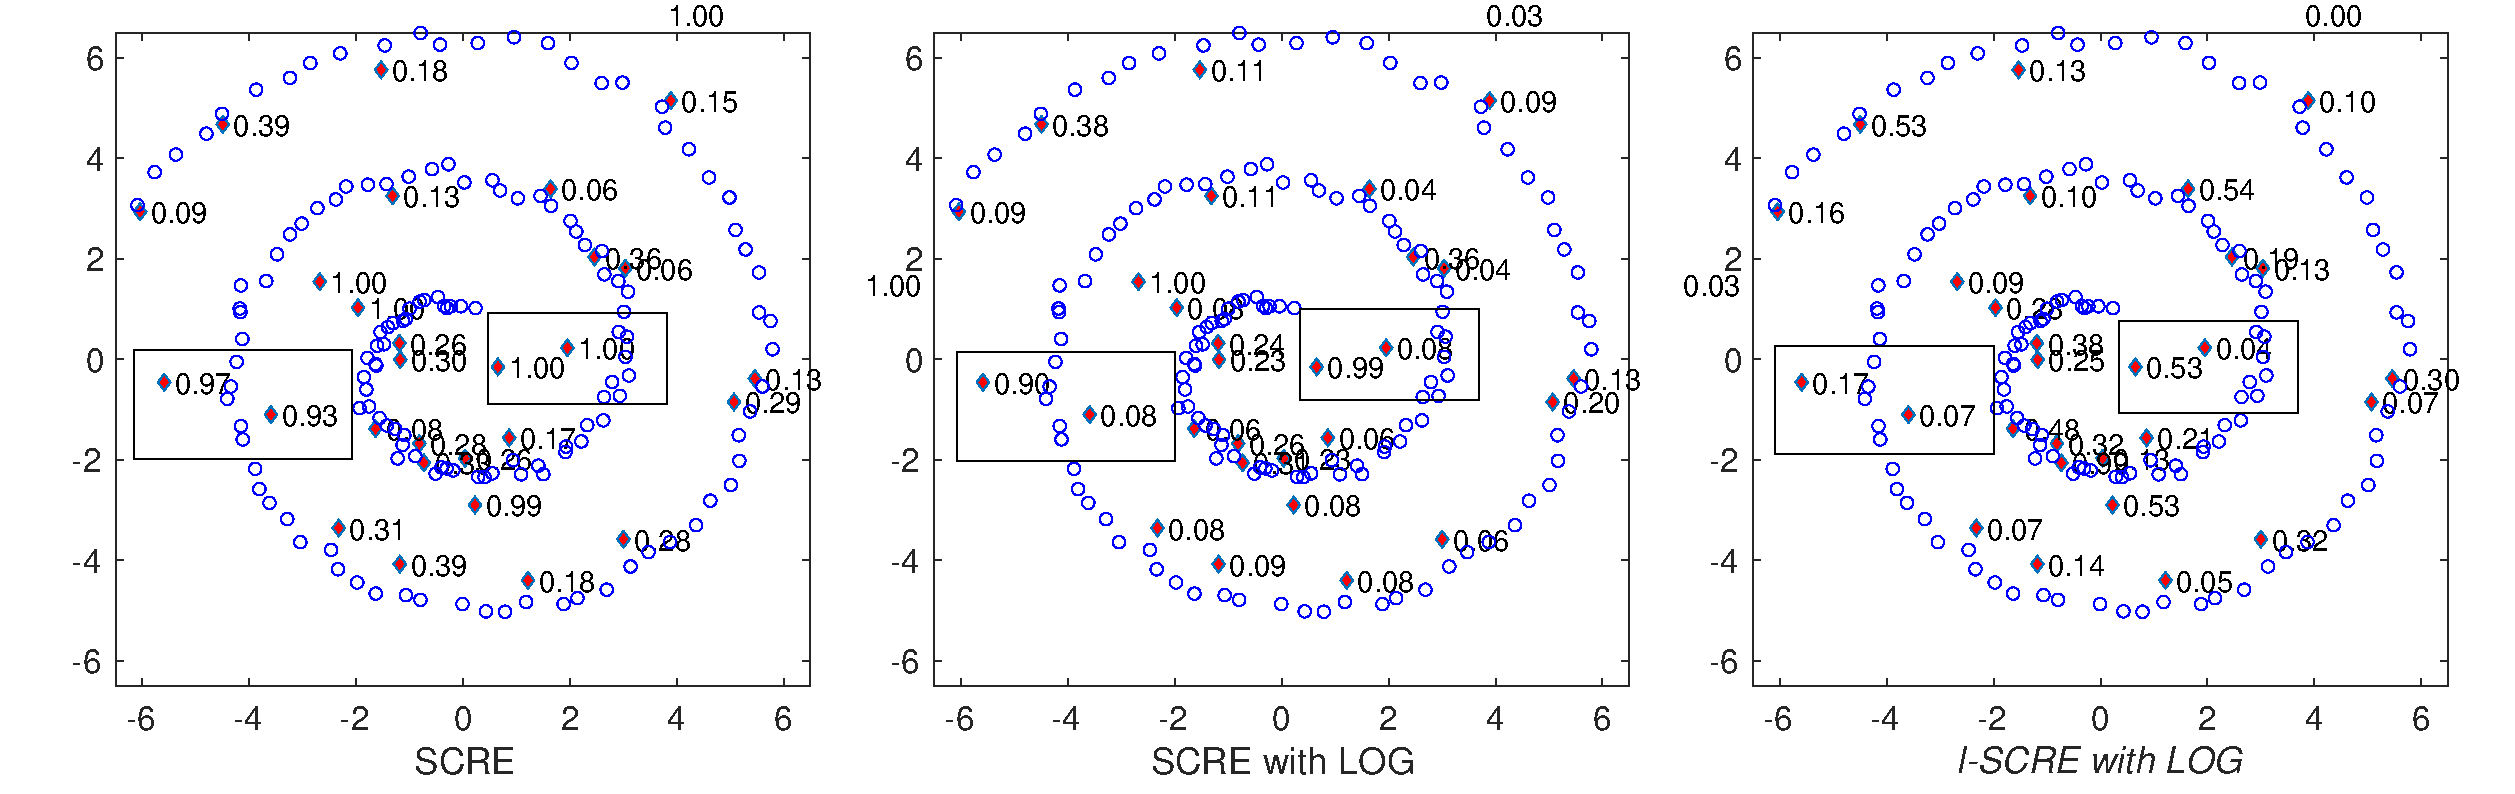
\includegraphics[width=\linewidth]{../figures/compare5.eps} 
    \caption{Illustration of the Performance of Three Difference Covariance Matrices }
    %\setcaptionwidth{6in}
    \label{fig:Diff Covariance}
 \end{figure}

 From Figure \ref{fig:Diff Covariance}, we can draw the following conclusions:
 \begin{itemize}
 \item As the left diagram shows, ${\rm s}(x)=1$ is a necessary but insufficient condition for $x$ to be on the ridge for KDE. The outliers that are far from the ridge may also make $s(x)=1$, which is the main disadvantage of obtaining the ridge by KDE without the nonlinear transformation. 
 \item Lemma \ref{rankonetheorem} is verified, as the values in the middle figure are all smaller than the corresponding values in the left figure.
\item The local version of KDE has a better property, especially for the values emphasized in the ellipse and rectangle shown in the right diagram. The outlier points have much smaller values of ${\rm s}(x)$ in the right diagram than those in the former two diagrams. 
 \end{itemize}
 
   \begin{figure} %  figure placement: here, top, bottom, or page
    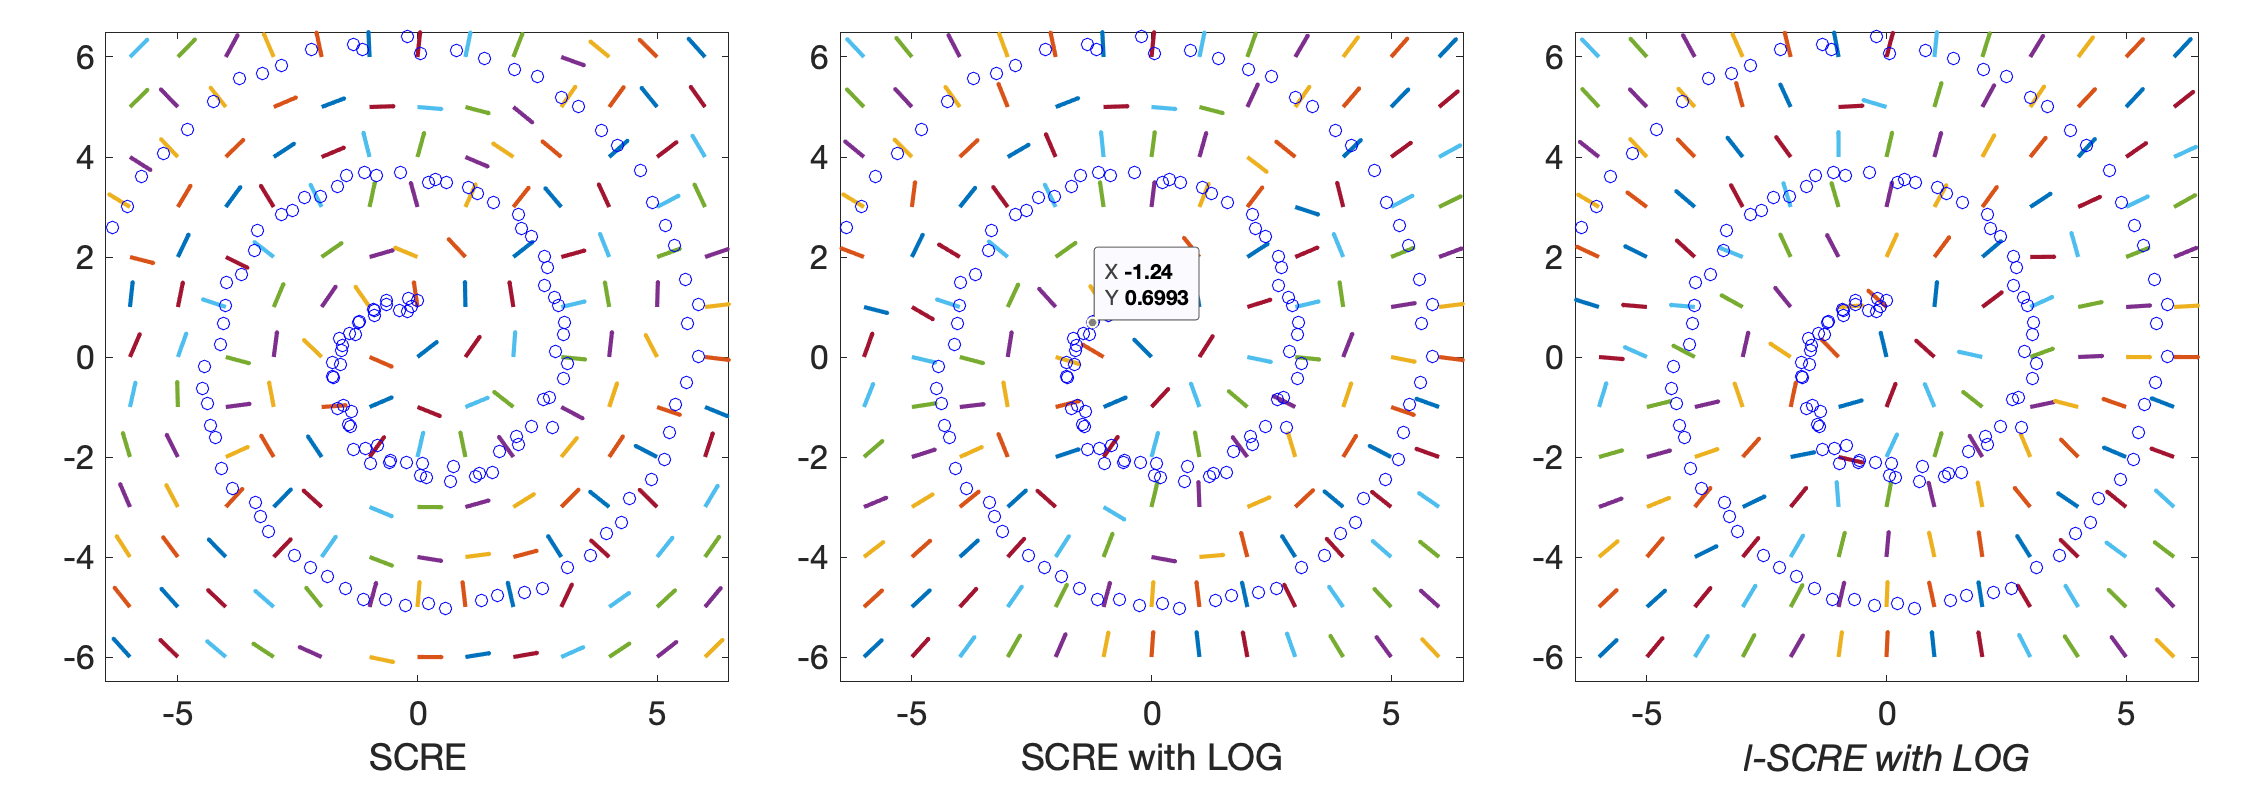
\includegraphics[width=\linewidth]{vectorfield.eps} 
    % \setcaptionwidth{6in}
    \caption{Illustration of the vector field corresponding to eigenvector of second eigenvalue with respect to three difference covariance matrices }
    \label{fig:vectorfield}
 \end{figure}
 In Figure \eqref{fig:vectorfield}, we plot the vector field generated by the eigenvector corresponding to the smallest eigenvalue. This vector field is the geometric interpretation of the projection $\Pi^{\perp}$ in the two-dimensional space. Because the constrained subspace in the two-dimensional space is one-dimensional, the vector field coincides with the trajectory of the outliers moving onto the ridge. We can conclude from the above figures that the vector field corresponding to LKDE is more smooth and points approximately to the projection onto the manifold, while the vector field of KDE is not well behaved for samples not close to the manifold.
\subsection{Synthetic Data Set}
First, we provide a one-dimensional ring example to show the effectiveness of our method compared with KDE. Because of the simplicity of the circle structure, it is easy to compute the projection onto it. We assume our hidden manifold ${\mathcal M}_c$ to be the one-dimensional circle embedded in a two-dimensional space with a radius of $1$ and center of $(0,0)$.

The observations are generated in the following two steps. First, a uniform sample from ${\mathcal M}_c$ is used to obtain the ideal observations without noise $y_k^*, k = 1:N$. Second, the independent noise from a two-dimensional normal distribution is added to get $y_k = y_k^*+\epsilon_k, k=1:N$. The observations are used to define our KDE and LKDE functions.

Generate a random mesh set $\mathcal G$ arbitrarily. For each point $x_k \in \mathcal G$, apply the subspace-constrained mean-shift algorithm to obtain a point $\tilde{x}_k$ that satisfies the ridge definition. Thus, the computed ridge set is ${\mathcal R}=\{\tilde{x}_k\}$. Because we use different approaches to define our ridge sets, we have ${\mathcal R}$ and ${\mathcal R}_\ell$, which correspond to the KDE and LKDE approaches.

For each point $\tilde{x}$ belonging to $\mathcal R$ or ${\mathcal R}_\ell$, we can define the projection of $\tilde{x}$ onto the real manifold $\mathcal M$ as $\pi_{\mathcal M}(\tilde{x}) = \arg\min_{y\in \mathcal M} \|y-\tilde{x}\|_2$. In the case of the special two-dimensional circle, the projection has an explicit form, $\pi_{\mathcal M}(\tilde{x}) = \tilde{x}/\|\tilde{x}\|$. The average margin from $\mathcal R$ or ${\mathcal R}_\ell$ to $\mathcal M$ is defined as
\[
{\rm Margin}({\mathcal R, \mathcal M}) =\frac{1}{|{\mathcal R}|}  \sum_{x_k\in \mathcal R} \min_{y\in \mathcal M}\|x_k-y\|_2.
\]

\begin{figure} %  figure placement: here, top, bottom, or page
   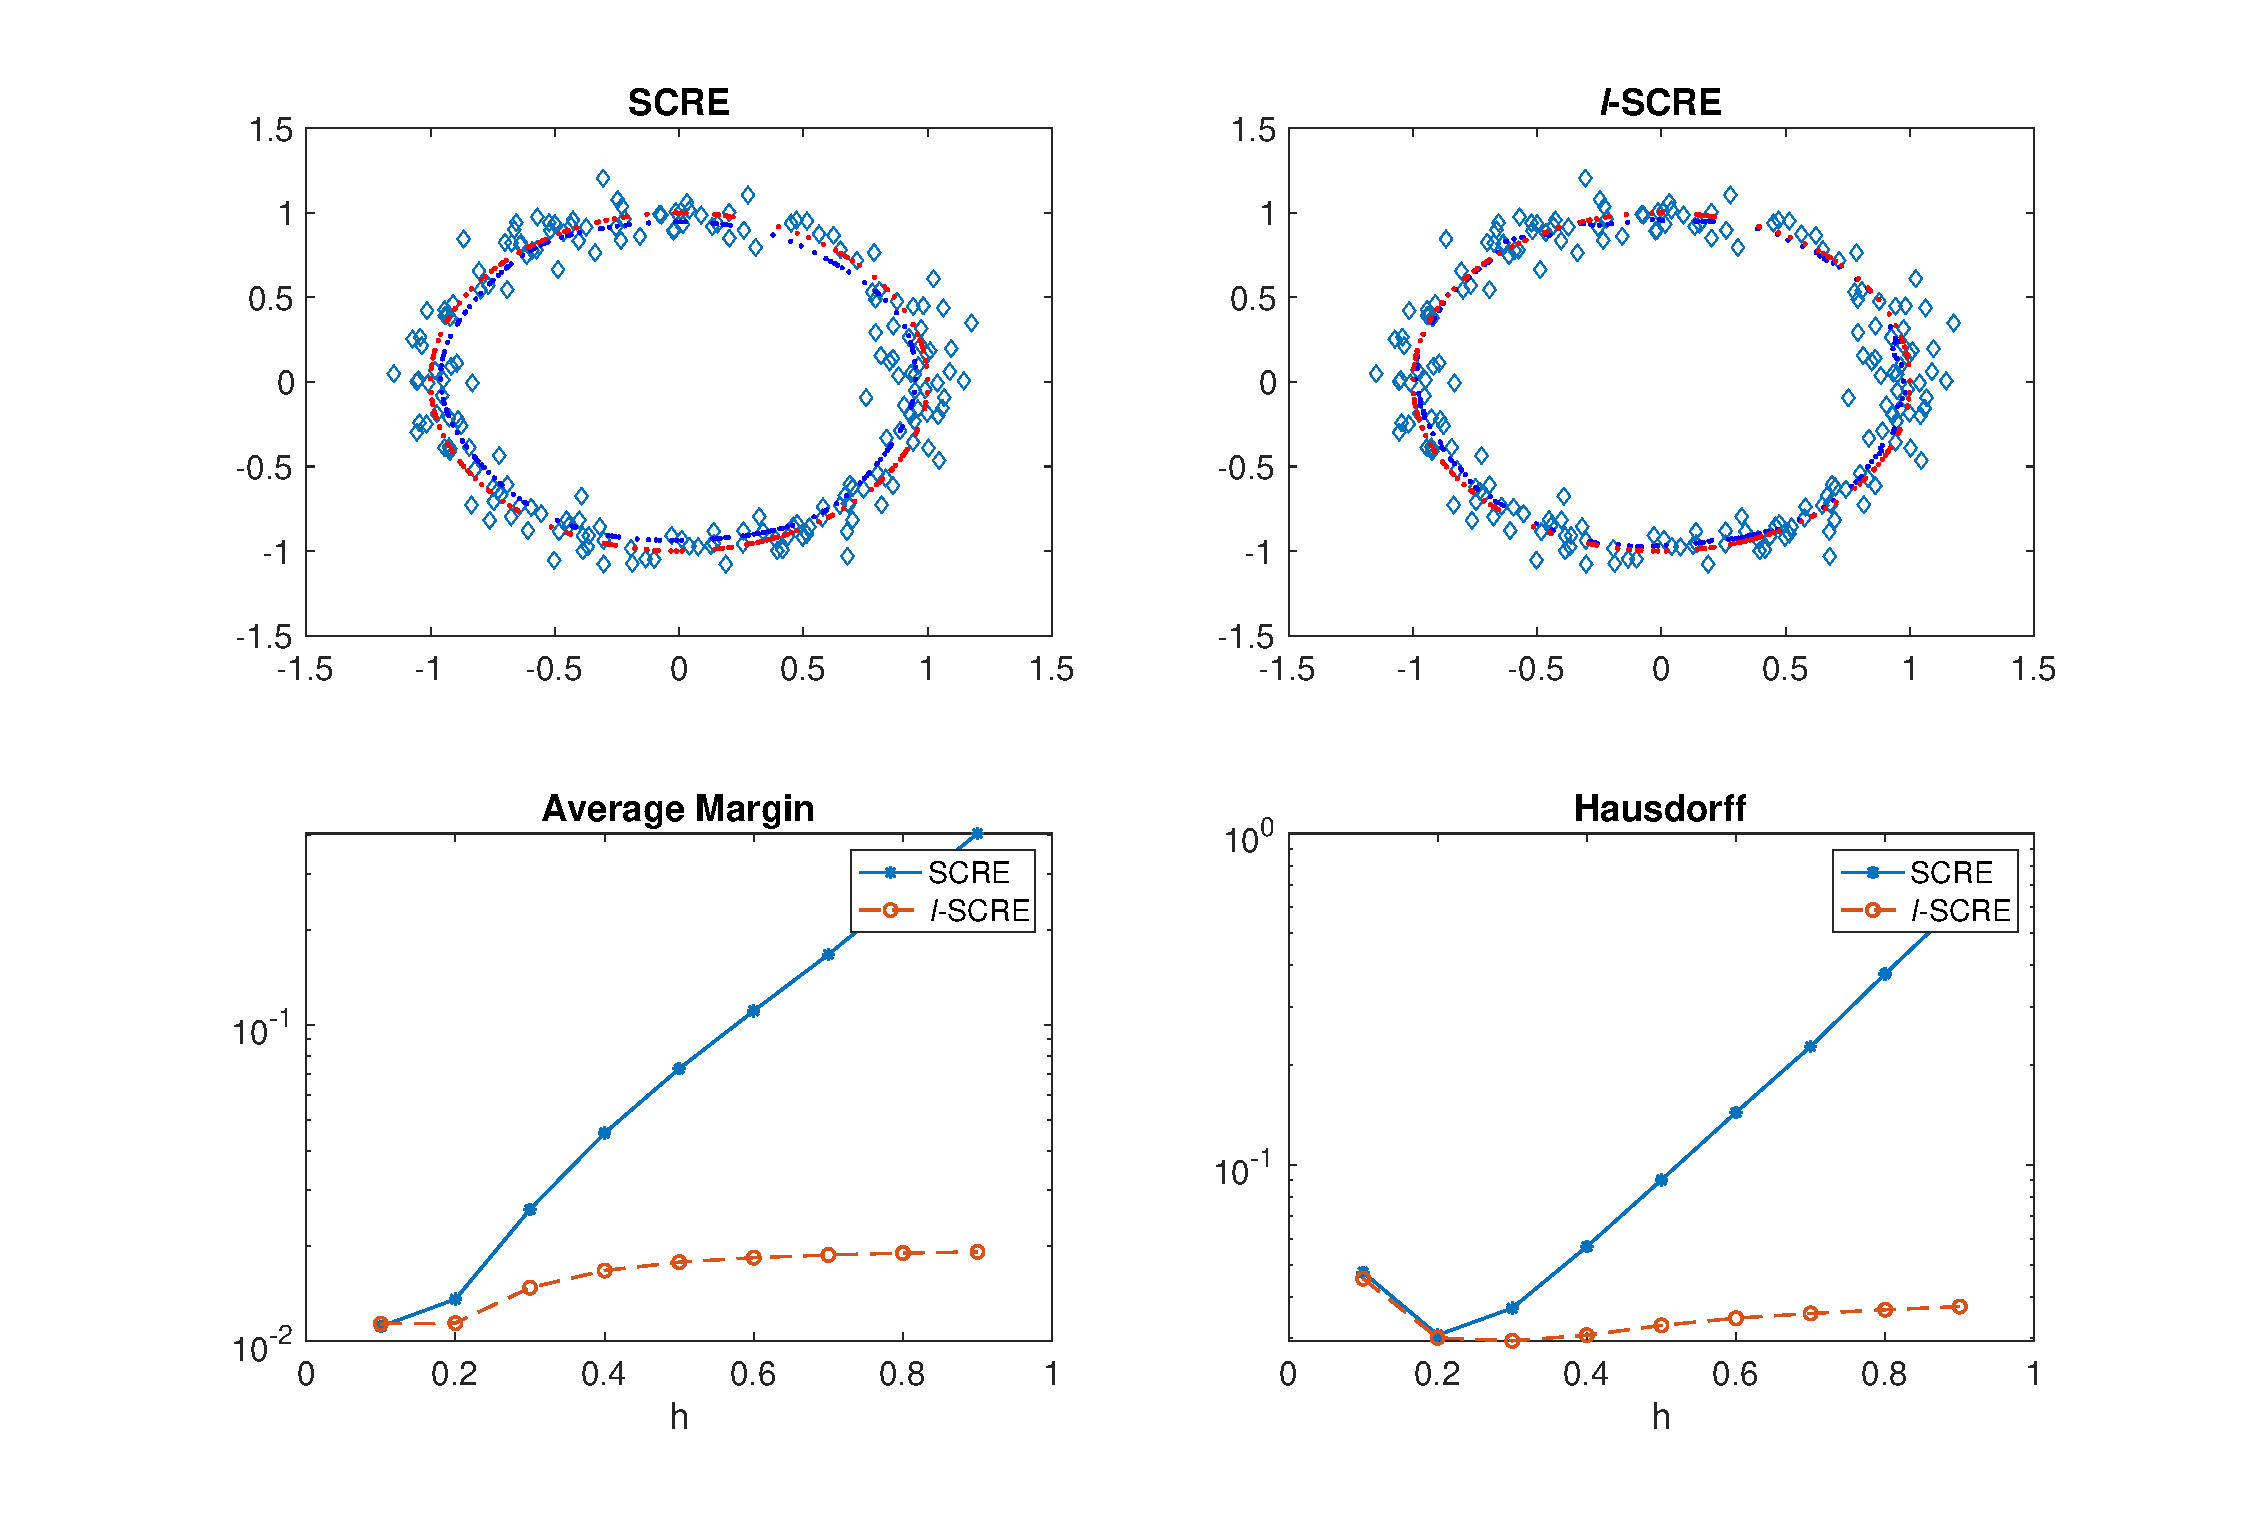
\includegraphics[width=\linewidth]{circle8.eps} 
   %\setcaptionwidth{6in}
   \caption{Margin Illustration for Ridges Obtained from LKDE and KDE}
   \label{fig:circle6}
\end{figure}
In Figure \ref{fig:circle6}, the small blue diamonds $\diamond$ represent the observations that are used to construct our KDE or LKDE function. The blue dots $\bullet$ represent the points that satisfy the ridge condition. The red dots $\bullet$ represent the projection of the blue dots onto the ideal manifold ${\mathcal M}_c$. Left: The margin of the ridge corresponding to KDE; Middle: The margin of the ridge corresponding to LKDE; Right: The average margin, which varies with the parameter $h$ when fixing the neighborhood size.

\begin{table}

\caption{The Margin of the Computed Ridge with $\mathcal M$ Varies with $h$ for KDE and LKDE}
\resizebox{12cm}{!}{
\begin{tabular}{c|c|ccccccccc}\hline
  & $h$   & 0.1   &0.2 &0.3 &0.4&0.5&0.6&0.7&0.8&0.9\\\hline
 %KDE  &0.0104&    0.0116  &  0.0240  &  0.0439  &  0.0714  &  0.1094  &  0.1656  &  0.2585  &  0.4220\\ \hline
 %LKDE&0.0103&    0.0113 &   0.0179&    0.0221&    0.0246&    0.0260 &   0.0269 &   0.0275 &   0.0279\\ \hline
 \multirow{2}{*}{Marg} &KDE  & 0.0121 &   0.0123 &   0.0246 &   0.0445  &  0.0716 &   0.1091 &   0.1648  &  0.2565 &   0.4274 \\ 
  &LKDE &  0.0118 &   0.0120 &   0.0182 &   0.0225 &   0.0249 &   0.0264 &    0.0272 &    0.0278 &   0.0283 \\ \hline
 \multirow{ 2}{*}{Haus} &KDE  &  0.0779 &   0.0333 &   0.0468 &   0.0662 &   0.0913 &   0.1307 &   0.1881 &   0.2837  &  0.4765 \\ 
 &LKDE & 0.0492 &   0.0329 &   0.0408 &   0.0456 &   0.0489  &  0.0510 &   0.0524 &   0.0534 &   0.0540 \\ \hline
\end{tabular}}
\label{table:margin}
\end{table}

It is clear from Table \ref{table:margin} and Figure \ref{fig:circle6} that, under the same parameter setting (such as $h$ and noise level $\sigma$), the algorithm of LKDE yields a ridge with a margin much smaller than that of KDE. The rate of increase of LKDE is much lower than that of KDE with the increase of $h$. This phenomenon is also explainable by our theoretical analysis.

\subsection{Real Data Set}
\begin{figure}[h] %  figure placement: here, top, bottom, or page
   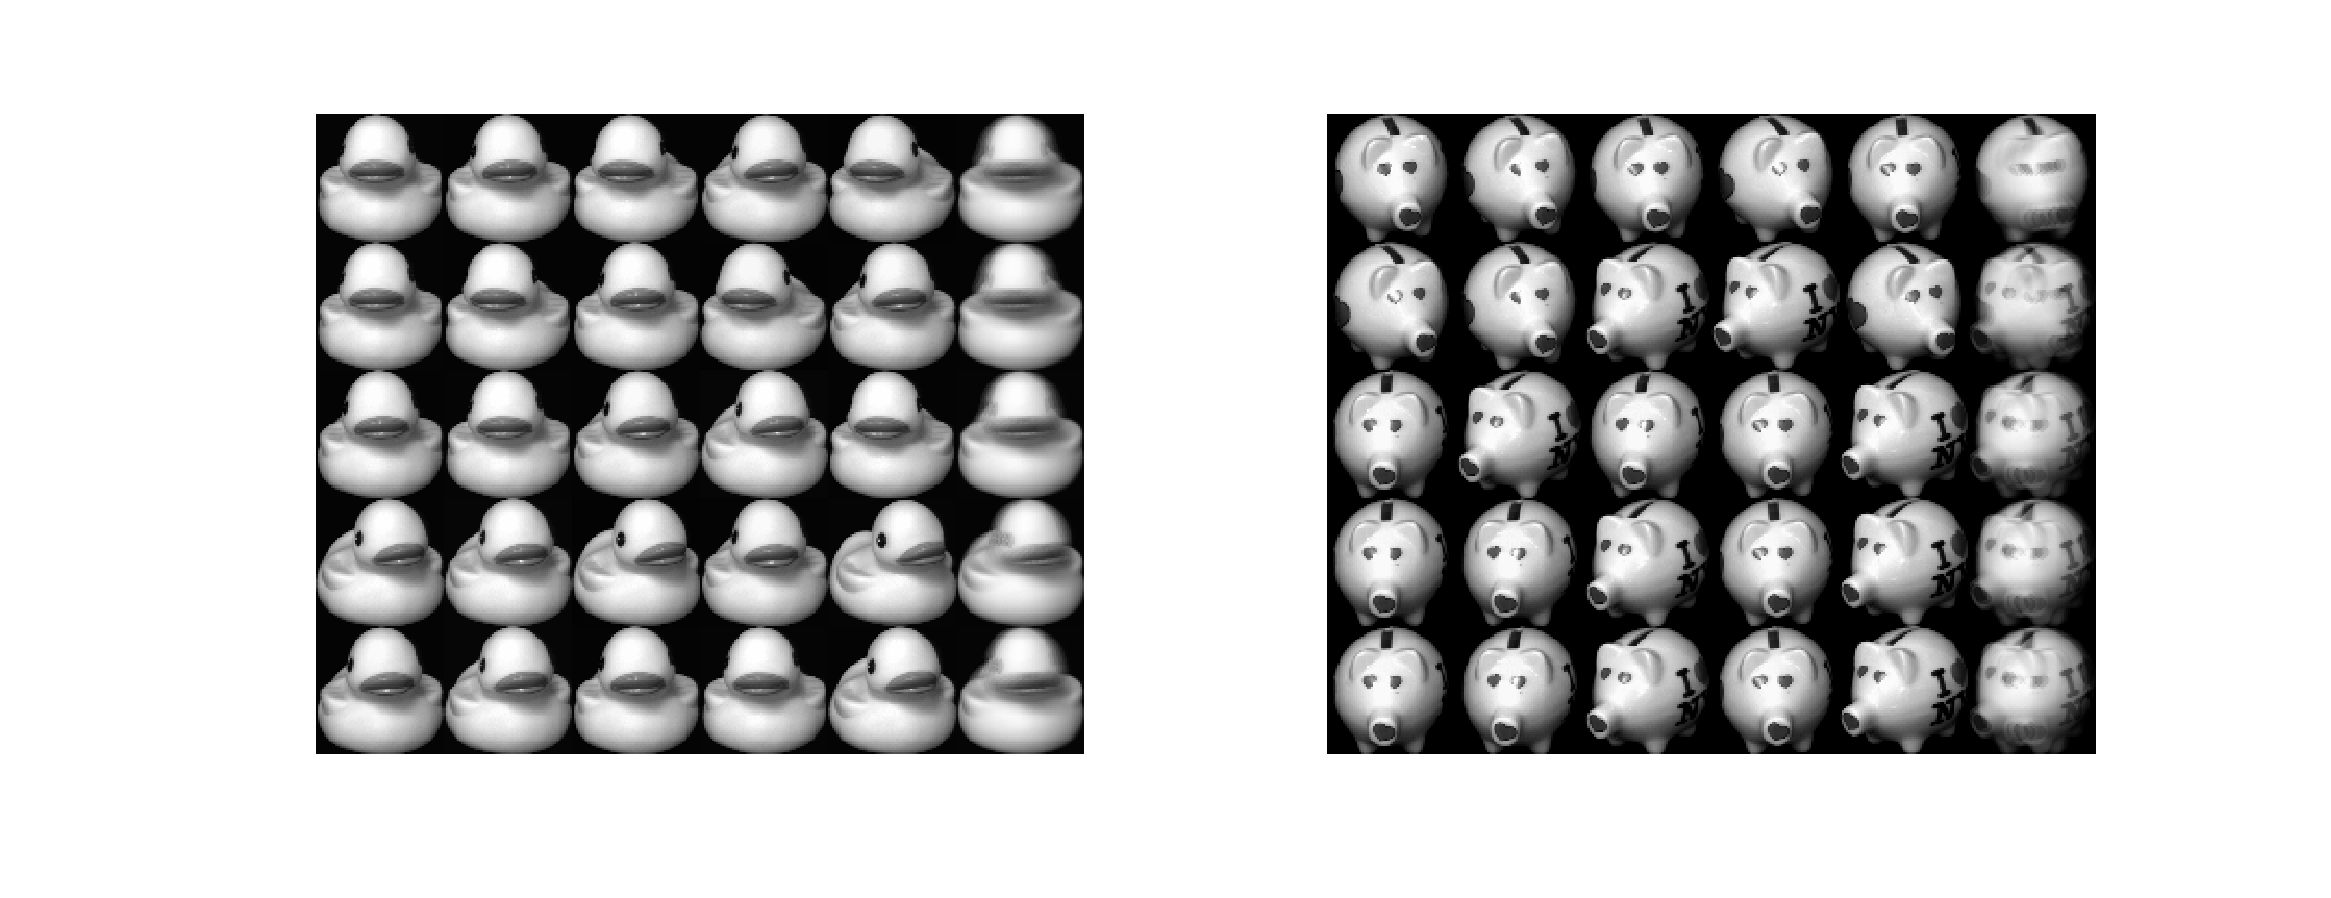
\includegraphics[width=\linewidth]{duck_pig.eps} 
   %\includegraphics[width=0.45\linewidth]{../figures/pig.eps} 
   \caption{Illustration of the interpolation for the one-dimensional Image Manifold}
   \label{fig:interpolation demo}
\end{figure}

We also test the performance of our algorithm using the Coil20 \cite{Coil20} dataset. The data is collected by rotating an object with 360 degrees. For each object, there are 72 images corresponding to a particular angle. Therefore, the images for each object can be supposed to reside on a one-dimensional manifold, since the underlying parameter is the angle.

Because we need to compute the eigenspace decomposition in the pixel space, the complexity is $O(n^3)$, where $n$ is the number of pixels. To reduce the complexity, we subsample each image with a $2\times 2$ window and obtain an image with the shape of $64\times 64$.

We randomly generate initial figures and use our algorithm to obtain an approximated image that is supposed to lie on the manifold. As Figure \ref{fig:interpolation demo} shows, the last column of each figure is the solution of an interpolation point corresponding to different initial figures. The five figures in the same line ahead of the interpolation figure are the five nearest neighborhoods.


\section{Discussion}
The manifold fitting is a challenging problem because of the unknown topology structure of the hidden manifold $\mathcal M$. We know only some observations that are supposed to be generated from $\mathcal M$ and also disturbed by some degree of noise. The main technique for handling the manifold-fitting problem is to focus on how to project an outlier observation (often disturbed by noise) onto its original uncontaminated manifold. The common approach is the subspace-constrained iteration or the subspace-constrained mean shifting.
Different algorithms differ in terms of the construction of the attraction force, the tangent space estimation, and some other factors. Based on the model assumption and the real data distribution, different approaches may vary to some degree in terms of performance.

\begin{appendix}
\section{}
\subsection{Ridge Derivative Lemma}
The following proof is a revised simple version of a similar proof in \cite{genovese2014nonparametric}. For completeness, we also include it in our paper.
\begin{proof}\label{Ridge Derivative Lemma}
 For two ridges $\hat{R}, R$, we have two density functions $\hat{p}(x)$ and $p(x)$ such that the points on each ridge satisfy the solution of
 $\Pi_{\hat{H}}(x) \hat{g}(x) = 0$ 
 and $\Pi_H(x) g(x) = 0$ respectively. For any starting point $\hat{x}\in \hat{R}$, we can build a unit speed curve $\gamma(s)$ derived from the gradient and Hessian of $p(x)$ as
 \[
 \gamma(0) = \hat{x} \in \hat{R}, \quad \gamma(t_0) = x_0 \in R, \quad \gamma'(s) = \frac{\Pi_H(\gamma(s))g(\gamma(s))}{\|\Pi_H(\gamma(s))g(\gamma(s))\|_2}.
 \]
Note that the curve $\gamma(t)$ connect $\hat{x}$ with $R$ by $x_0$. Define the univariate function $\xi(s)$ as
  \[
  \xi(s) = p(\gamma(t_0))-p(\gamma(s)), \quad 0<s<t_0.
  \]
Through a simple computation, we know 
 \[
 \xi'(s)=-\langle  g(\gamma(s)), \gamma'(s) \rangle =- \|\Pi_H(\gamma(s))g(\gamma(s))\|_2, \quad \xi'(t_0) = 0.
 \]
 %\[
 %\xi''(s) = \frac{\langle L_{\gamma'(s)}(\gamma(s)) g(\gamma(s)), L(\gamma(s)g(\gamma(s)))\rangle}{\|L(\gamma(s))g(\gamma(s))\|_2}
 %\]
 %with $\gamma(s)=\frac{L(\gamma(s)g(\gamma(s)))}{\|L(\gamma(s)g(\gamma(s)))\|}$
 The distance from $\hat{x}$ to $R$ can be bounded by the curve length of $\gamma(t)$ which is $t_0$
 \[
 d(\hat{x}, R) = \|\hat{x}-P_R(\hat{x})\|_2\leq \|\hat{x}-x_0\|_2 = \|\gamma(t_0)-\gamma(0)\|_2\leq t_0.
 \]
Finally, the problem becomes to bound $t_0$. Suppose $\sup_u \xi''(u)>\frac{1}{c}$, by the mean-value theorem, we have
 \[
 t_0 = \frac{\xi'(t_0)-\xi'(0)}{\xi''(u)} = \frac{\|\Pi_H(\gamma(0))g(\gamma(0))\|_2}{\xi''(u)} \leq c \|\Pi_H(\gamma(0))g(\gamma(0))\|_2.
 \]
 Next, we show that $\|\Pi_H(\gamma(0))g(\gamma(0))\|_2$ is of the same order with an approximation error of $H(x)$ and $g(x)$:
 \[
 \begin{aligned}
 \|\Pi_H(\gamma(0))g(\gamma(0))\|_2=&  \|\Pi_H(\gamma(0))g(\gamma(0)) - \Pi_{\hat{H}}(\gamma(0))\hat{g}(\gamma(0))\|_2\\
 \leq & \|\Pi_H(\gamma(0))g(\gamma(0)) -\Pi_{\hat{H}}(\gamma(0)){g}(\gamma(0)) \|_2 +...\\
 & + \|\Pi_{\hat{H}}(\gamma(0)){g}(\gamma(0)) - \Pi_{\hat{H}}(\gamma(0))\hat{g}(\gamma(0))\|_2\\
 \leq & \|\Pi_H(\gamma(0)) - \Pi_{\hat{H}}(\gamma(0))\|_F\|g(\gamma(0))\|_2 +...\\
 &+\|\Pi_{\hat{H}}(\gamma(0))\|_F\|g(\gamma(0))-\hat{g}(\gamma(0))\|_2, \\
 \end{aligned}.
 \]
 where the last inequality is obtained by applying the Cauchy-Schwartz inequality on each row of $A$, to get the result $\|Ax\|_2\leq \|A\|_F\|x\|_2$. According to the Davis-Kahan theorem, $\|\Pi_H(\gamma(t))-\Pi_{\hat{H}}(\gamma(t))\|_F \leq \beta\|H(\gamma(t))-\hat{H}(\gamma(t))\|_F$. The conclusion is proved!
\end{proof}


\subsection{Derivatives' Bias Bound}\label{bias_proof}
\begin{proof}
Suppose the kernel function vanishes at infinity for each dimension, i.e., it satisfies $\lim_{u_s\rightarrow \infty}K(u)=0$ for each dimension. Then, using the integration-by-parts formula, we obtain the expectation of first-order derivatives:
\begin{equation}\label{Expectation}
\begin{aligned}
{\rm E} (\partial_{x_s} \hat{p}_n(x)) &= \frac{1}{h^D} \int_{y\in \mathbb{R}^D}{\partial_{x_s}}  K(\frac{x-y}{h}) p(y) dy  \\
&=\frac{1}{h^{D+1}}\int \partial_{z_s} K(z)|_{z=\frac{x-y}{h}} p(y) dy=h^{-1} \int_ {u\in \mathbb{R}^D} \partial_{u_s} K(u) p(x-hu)  d u\\
&=h^{-1}\int_ {u\in \mathbb{R}^D} K(u) \partial_{u_s} p(x-hu) d u = \int_ {u\in \mathbb{R}^D} K(u) \partial_{z_s}p(z)|_{z=x-hu} d u.
\end{aligned}
\end{equation}
For the multivariate function $\partial_{x_s} p(x)$, we have the Taylor expansion up to order 2 as
\begin{equation}\label{Taylor}
\partial_{z_s} p(z)|_{z=x-hu}= \partial_{x_s} p(x) -  h u^T\nabla \partial_{x_s} p(x) + \frac{1}{2}h^2 u^T H(\partial_{x_s}p(x))u + o(h^2).
\end{equation}
Since $u^T \nabla \partial_{x_s} p(x) K(u)$ is an odd function with respect to each variable $u_s$, we have the integration $\int u^T \nabla \partial_{x_s} p(x) K(u) du = 0 $ in a symmetric region. As a consequence, we know the bias
\begin{equation}\label{BiasResult}
|{\rm E}(\partial_{x_s} \hat{p}_n(x)) - \partial_{x_s}p(x)|  \leq \frac{\lambda_s(x)}{2} h^2 \int \|u\|_2^2 K(u) du+o(h^2),
\end{equation}
where $\lambda_s(x)$ is the largest eigenvalue of the Hessian matrix $H(\partial_{x_s}p(x))$. Similarly, repeating the same procedure as \eqref{Expectation}\eqref{Taylor}, we have the second-order bias as
\begin{equation}\label{order2}
|{\rm E}( \partial_{x_s} \partial_{x_t}   \hat{p}_n(x)) -  \partial_{x_s} \partial_{x_t} p(x)| \leq \frac{\lambda_{st}(x)}{2} h^2 \int \|u\|_2^2 K(u) du+o(h^2).
\end{equation}
The same with \eqref{BiasResult}, $\lambda_{st}(x)$ is the largest eigenvalue of the matrix $M_{st}$ whose $i,j$-th element is $\frac{\partial^4}{\partial x_s\partial x_t \partial x_i \partial x_j} p(x)$, i.e., $\lambda_{st}(x)= \max_k \lambda_k( M_{st}(x))$.
\end{proof}
\subsection{Derivatives' Variance Bound}\label{variance_proof}
\begin{proof}
Because of the i.i.d. assumption and the characters of the variance, the first-order derivative yields
\[
\begin{aligned}
 &{\rm Var} (\partial_{x_s} \hat{p}_n(x))  = {\rm Var} (\frac{1}{n h^D}\sum_k \partial_{x_s}(K(\frac{x-y_k}{h})))\\
  = &\frac{1}{n h^{2D}} {\rm Var}(  \partial_{x_s} K(\frac{x-y}{h}))))=  \frac{1}{n h^{2D+2}} {\rm Var} (\partial_ {u_s}  K(u)|_{u=\frac{x-y}{h}}).%= \frac{1}{n h^{2d+4}} (E_y({k^{''}}^2_{rs}(\frac{x-y}{h}))- E_y^2(k^{''}_{rs}(\frac{x-y}{h}))
\end{aligned}
\]
Next, we derive the variance by using the equality of variance and expectation ${\rm Var}(a) = {\rm E}(a^2)-{\rm E}^2(a)$.
In addition, let $M(\frac{x-y}{h}) = \partial_ {u_s}  K(u)|_{u=\frac{x-y}{h}}$, which will lead to
\begin{equation}\label{e11}
 {\rm Var} (\partial_{x_s} \hat{p}_n(x)) = \frac{1}{nh^{2D+2}}({\rm E}_y (M^2(\frac{x-y}{h}))-{\rm E}^2_y(M(\frac{x-y}{h}))).
%\frac{1}{h^d}\int M(\frac{x-y}{h}) p(y)dy = \int M(u)p(x-uh) du=p(x) \int M(u) du+O(h)
\end{equation}
Noting the bias result from \eqref{Expectation} and \eqref{BiasResult}, we have
\begin{equation}\label{EM}
\begin{aligned}
&{\rm E}_y(M(\frac{x-y}{h})) \\
= &h^{D+1} ( {\rm E}(\partial_{x_s} \hat{p}_n(x))\leq h^{D+1} (\partial_{x_s} p(x)+\frac{\lambda_s(x)}{2} h^2 \int \|u\|^2 K(u) du+o(h^2)).
\end{aligned}
\end{equation}
Taking the square of \eqref{EM} on both sides, we obtain
\[
{\rm E}^2_y(M(\frac{x-y}{h})) = h^{2D+2}((\partial_{x_s} p(x))^2+ O(h^2)).
\]
Taking the expectation of $M^2(\frac{x-y}{h})$, and changing the variable $u=\frac{x-y}{h}$, we obtain
\begin{equation}\label{part1}
{\rm E}_y(M^2(\frac{x-y}{h})) = \frac{1}{h^D} \int M^2(u) p(x-uh) du = \frac{1}{h^D}(p(x)\int M^2(u)du+O(h)).
\end{equation}
Using \eqref{EM},\eqref{part1} we have
\begin{equation}\label{Var}
\begin{aligned}
  & {\rm Var} (\partial_{x_s} \hat{p}_n(x))  \\
=& \frac{1}{n h^{2D+2}}({\rm E}_yM^2(\frac{x-y}{h}))-{\rm E}^2_y(M(\frac{x-y}{h})) = \frac{1}{n h^{D+2}} (p(x)\int M^2(u)du +O(h)).
\end{aligned}
\end{equation}
%We noted that
%\[
%{\rm Var}(\partial_{x_s}p_n(x)) = {\rm E}(\partial_{x_s} p_n(x)-{\rm E}(\partial_{x_s} p_n(x)))^2
%\]
Because the square-root function is concave, we use Jensen's inequality to determine that
\begin{equation}\label{Jensen}
\sqrt{{\rm Var}(\partial_{x_s}\hat{p}_n(x))} = \sqrt{{\rm E}(\partial_{x_s} p_n(x)-{\rm E}(\partial_{x_s} p_n(x)))^2}\geq {\rm E} |\partial_{x_s} \hat{p}_n(x)-{\rm E}(\partial_{x_s} \hat{p}_n(x))|.
\end{equation}
Combining \eqref{Var} and \eqref{Jensen} yields
\begin{equation}\label{VarResult}
{\rm E} |\partial_{x_s} \hat{p}_n(x)-{\rm E}(\partial_{x_s} \hat{p}_n(x))| \leq \sqrt{\frac{p(x)\int M^2(u)du}{n h^{D+2}}}.
\end{equation}
%From \eqref{error2}, we have
%\begin{equation}\label{expectationd2}
%E_y^2(k^{''}_{rs}(\frac{x-y}{h}) =n h^{2d+4}({\{p^{(2)}_{rs}(x)\}}^2+O(h^2))
%\end{equation}
%Let $M(u) = \max_{r,s} (\partial_{r,s} k(u))^2$. Using \eqref{e1}\eqref{expectationd2} , we have
Repeating the procedures \eqref{e11} - \eqref{Jensen},  we obtain
\begin{equation}\label{VarResult2}
{\rm E} | \partial_{x_s}\partial_{x_t} \hat{p}_n(x) -\partial_{x_s}\partial_{x_t} p(x)| \leq \sqrt{\frac{p(x)\int N^2(u)du}{nh^{D+4}}},
\end{equation}
%\[
%|f_n^{(1)}(x) - p^{(1)}(x)|\leq \frac{C}{2} h^2 \int \|u\|^2 k(u) du +\sqrt{\frac{p(x)\int N^2(u)du}{nh^{d+2}}}
%\]
where $N(\frac{x-y}{h}) $ is defined as $N(\frac{x-y}{h}) = \partial_ {u_s}\partial_{u_t}  K(u)|_{u=\frac{x-y}{h}}$ in a similar way.
\eqref{VarResult} and \eqref{VarResult2} have different orders with respect to $h$, which could lead to an optimal-parameter dilemma, as shown in the next section.
\end{proof}
\subsection{Derivatives' Bias for LKDE}
\begin{proof}\label{LKDE bias}
Recall that, in the bias for kernel density estimation, we also have the expression of expectation and the Taylor expansion:
\[
\begin{aligned}
&{\rm E} (\partial_{x_s} \hat{p}_{r,h}(x)) = \int_ {u\in \mathbb{R}^D} K_r(u) \partial_{z_s}p(z)|_{z=x-hu} d u,\\
&\partial_{z_s} p(z)|_{z=x-hu}= \partial_{x_s} p(x) -  h u^T\nabla \partial_{x_s} p(x) + \frac{1}{2}h^2 u^T H(\partial_{x_s}p(x))(x)u + o(h^2).
\end{aligned}
\]
Thus, we have
\begin{equation}\label{biasn1}
{\rm E} (\partial_{x_s} \hat{p}_{r,h}(x))  \leq \partial_{x_s} p(x) \int_ {u\in \mathbb{R}^D} K_r(u) du + \frac{\lambda_s(x)}{2} h^2 \int_{\|u\|\leq r/h } \|u\|_2^2 K(u) du + o(h^2).
\end{equation}
Note that $\int_{u\in \mathbb{R}^D} K_r(u) du=\int_{\|u\|\leq r/h} K(u) du$ and 
\[
\int_{\|u\|\leq r/h} K(u) du + \int_{\|u\|> r/h} K(u)du =1.
\]
Subtracting $\partial_{x_s}p(x)$ in \eqref{biasn1} from both sides, we have
\begin{equation}\label{biasn2}
\begin{aligned}
&|{\rm E}( \partial_{x_s} \hat{p}_{r,h}(x)) -  \partial_{x_s} p(x)| \\
\leq &
|\partial_{x_s} p(x)| \int_{\|u\|\geq r/h} K(u) du  + \frac{\lambda_s(x)}{2} h^2 \int_{\|u\|\leq r/h } \|u\|_2^2 K(u) du .
\end{aligned}
\end{equation}
Comparing \eqref{biasn2} with \eqref{BiasResult}, we reduce the term $\frac{\lambda_s(x)}{2} h^2 \int \|u\|_2^2 K(u) du$ to the bounded scope as $\frac{\lambda_s(x)}{2} h^2 \int_{\|u\|\leq r/h } \|u\|_2^2 K(u) du$ by introducing an extra term $|\partial_{x_s} p(x)| \int_{\|u\|> r/h} K(u) du$. Next, we compare the two terms. It can be easily observed that, to reduce the bias, we only need to make sure the following inequality is satisfied:
\begin{equation}\label{Necessary}
\frac{\lambda_s(x)}{2} h^2 \int_{\|u\|> r /h} \|u\|_2^2 K(u) du > |\partial_{x_s} p(x)| \int_{\|u\|> r/h} K(u) du.
\end{equation}
When $r>h$, we have $\|u\|>1$, and thus $\frac{ \int_{\|u\|> r /h} \|u\|_2^2 K(u) du}{ \int_{\|u\|> r/h} K(u) du}\geq r^2/h^2$. Furthermore, if we choose $r$ such that $r^2/h^2\geq\frac{2|\partial_{x_s} p(x)|}{\lambda_s(x) h^2}$, the sufficient  condition for \eqref{Necessary} will be met.
\end{proof}

\subsection{Simplified Bias Result}
\begin{proof}\label{Simplified Bias Result}
From comparison \eqref{BiasResult} and \eqref{order11}, we know that if 
\[
\frac{\lambda_s(x)}{2} h^2 \int_{\|u\|\geq r /h} \|u\|_2^2 K(u) du >  \int_{\|u\|\geq r/h} K(u) du |\partial_{x_s} p(x)|,
\]
the bias of $\partial_{x_s} p_{r, h}(x), \partial_{x_s} \partial_{x_t} p_{r, h}(x)$ will be reduced through replacement of the LKDE with the KDE in \eqref{GKDE}.
Define
\[
\begin{aligned}
&\gamma = \frac{\int_{\|u\|\geq r/h } \|u\|_2^2 K(u) du}{ 2\int_{\|u\|\geq r/h} K(u) du },\\
&\mu_s(x) = \frac{\lambda_s(x) h^2 \int_{\|u\|\leq r /h} \|u\|_2^2 K(u) du +  2\int_{\|u\|\geq r/h} K(u) du |\partial_{x_s} p(x)|}{\lambda_s(x) h^2 \int\|u\|_2^2 K(u) du }.
\end{aligned}
\]
Clearly, when $r/h \geq 1$, we have $\gamma\geq 1/2$. As a result, we can provide a sufficient condition for which using the LKDE is better than KDE for the bias reduction. 
\end{proof}
\subsection{Derivatives' Variance for LKDE}
\begin{proof}\label{Derivatives' Variance for LKDE}
Because of ${{\rm Var}}(u) = {\rm E}(u - {\rm E}u)^2 = {\rm E}(u^2) - ({\rm E}(u))^2$, by neglecting the low order  term $({\rm E}(u))^2$,  we have
\begin{equation}\label{step1}
{{\rm Var}}(\partial_{x_s} \hat{p}_{r,h}(x)) \leq {\rm E} ((\partial_{x_s} \hat{p}_{r,h}(x))^2) .
\end{equation}
Also noting that $\hat{p}_{r,h}(x)=\frac{1}{n h^D} \sum_k K_r(\frac{x-x_k}{h})$ and taking the expectation with respect to the random variable $x_k$, we have
\begin{equation}\label{step2}
 {\rm E} ((\partial_{x_s} \hat{p}_{r,h}(x))^2) = \frac{1}{n h^{2D}} {\rm E}_y ((\partial_{x_s } K_r (\frac{x - y}{h}))^2).
\end{equation}
Using \eqref{DTK}, we have
\begin{equation}\label{step3}
\frac{1}{n h^{2D}} {\rm E}_y ((\partial_{x_s } K_r (\frac{x - y}{h}))^2) \leq \frac{1}{n h^{2D}} {\rm E}_y ((\partial_{x_s } K(\frac{x - y}{h}))^2).
\end{equation}
Because of the chain rule of derivatives, we have
\begin{equation}\label{step4}
\frac{1}{n h^{2D}} {\rm E}_y ((\partial_{x_s} K(\frac{x - y}{h}))^2) = \frac{1}{n h^{2D+2}} \int (\partial_{u_s } K (u) |_{u=\frac{x - y}{h}})^2 p(y) dy.
\end{equation}
Using the rule for changing the integrating variable from $y$ to $u$, we have 
\begin{equation}\label{step5}
\frac{1}{n h^{2D+2}} \int (\partial_{u_s } K (u) |_{u=\frac{x - y}{h}})^2 p(y) dy = \frac{1}{n h^{D+2}} \int (\partial_{u_s } K (u) )^2 p(x-uh) du.
\end{equation}\label{step6}
In the same way as before, by Taylor expansion $p(x-uh)=p(x)+O(h)$, we have
\begin{equation}\label{step7}
\frac{1}{n h^{D+2}} \int (\partial_{u_s } K (u) )^2 p(x-uh) du = \frac{1}{n h^{D+2}}  (p(x) \int (\partial_{u_s } K (u) )^2   du + O(h)).
\end{equation}
Combining the inequalities in \eqref{step1}-\eqref{step7}, we can obtain the result.
\end{proof}
\subsection{Minimum Relation}
\begin{proof}\label{mimimum_proof}
For a function $\nu(h) = a_0 h^2 + a_1 \sqrt{\frac{1}{nh^{D+m}}}, m=2,4$, the global optimal minimum is achieved at $h^* = 
%\arg\min_h \nu(h) = 
(\frac{a_1^2}{n a_0^2})^{\frac{1}{D+m+4}}$, with the function value being
\[
\nu(h^*) = 2(\frac{a_1^2 a_0^{\frac{D+m}{2}}}{n})^{\frac{2}{D+m+4}}=2 a_0^{\frac{D+m}{D+m+4}} a_1^{\frac{1}{D+m+4}} {n}^{-\frac{2}{D+m+4}}.
\]
Consider another function by replacing $a_0$ in $\nu(h)$ with $\mu a_0$, where $\mu\in(0,1)$
\begin{equation}\label{f_mu}
\nu_\mu (h) = \mu a_0 h^2 + a_1 \sqrt{\frac{1}{nh^{D+m}}}.
\end{equation}
The modified function $\nu_\mu(h)$ will lead to a new minimum optimum point as
\[
h^{**} =\arg\min \nu_\mu( h)=(\frac{a_1^2}{n \mu^2 a_0^2})^{\frac{1}{D+m+4}}.
\] 
Substituting it into \eqref{f_mu}, by a simple calculation, we obtain $\nu_\mu (h^{**}) = \mu^{\frac{D+m}{D+m+4}}\nu(h^*)$.
Since $\frac{D+4}{D+8}>\frac{D+2}{D+6}$ and $\mu^x$ is a decreasing function for $\mu\in (0,1)$, we have $\max\{\mu^{\frac{D+4}{D+8}}, \mu^{\frac{D+2}{D+6}}\} = \mu^{\frac{D+2}{D+6}}$. 
\end{proof}
\section{}
\subsection{Rank-one Enlarge Projection}
\begin{proof}\label{Rank-one Enlarge Projection}
Because of the variational inequality of eigenvectors, the top $d$ eigenvectors can be written as the solution of the maximum optimal problem
 \[
U_A = \arg\max_{U^TU = I_d} {\rm trace} (U^T A U), \quad U_B = \arg\max_{U^TU = I_d} {\rm trace} (U^T B U).
\]
Denote $\Pi_A = U_A {U_A}^T,  \Pi_B = U_B {U_B}^T$, we have 
\begin{equation}\label{variantional}
\langle \Pi_B , B \rangle \geq \langle \Pi_A , B \rangle,  \quad \langle \Pi_A , A \rangle \geq \langle \Pi_B , A \rangle.
\end{equation}
Using \eqref{variantional}, we have
\[
\begin{aligned}
&\langle \Pi_B, B\rangle+ \langle \Pi_A, \lambda uu^T\rangle\\
 \geq &\langle \Pi_A, B+\lambda uu^T \rangle = \langle \Pi_A , A \rangle   \geq  \langle \Pi_B, B+\lambda uu^T \rangle =  \langle \Pi_B, B\rangle + \langle \Pi_B, \lambda uu^T \rangle.
\end{aligned}
\]
Eliminating the constant $\langle \Pi_B, B\rangle$ on both sides, we have $\langle  \Pi_A , uu^T\rangle \geq  \langle  \Pi_B,  uu^T\rangle$. Since 
\[
\langle \Pi_A, uu^T \rangle= u^T \Pi_A u = u^T \Pi_A \Pi_A u = \|\Pi_A u\|_2^2,
\] 
As a consequence, we have $\|\Pi_A u\|_2\geq \|\Pi_B u\|_2$.
\end{proof}
\subsection{Inclusion Theorem}
\begin{proof}
For any two projections $\Pi_{H_p}(x), \Pi_{H_{f(p)}}(x)$ and their orthogonal complement projection $\Pi^\perp_{H_p}(x), \Pi^\perp_{H_{f(p)}}(x)$, we have the following two equalities:
\[
\begin{aligned}
&\|\Pi_{H_p}^{\perp}(x) \nabla p(x)\|_2^2 +\|\Pi_{H_p}(x) \nabla p(x)\|_2^2 = \|\nabla p(x)\|_2^2,\\
&\|\Pi_{H_{f(p)}}^{\perp}(x) \nabla p(x)\|_2^2 +\|\Pi_{H_{f(p)}}(x) \nabla p(x)\|_2^2 = \|\nabla p(x)\|_2^2.
\end{aligned}
\] 
Note that $\|\Pi_{H_p}^{\perp}(x)\nabla p(x)\|_2 \leq \|\Pi_{H_{f(p)}}^{\perp}(x)\nabla p(x)\|_2$ is equivalent to \[
\|\Pi_{H_p}(x)\nabla p(x)\|_2 \geq \|\Pi_{H_{f(p)}}(x)\nabla p(x)\|_2.\] To prove $\|\Pi_{H_p}(x)\nabla p(x)\|_2 \geq \|\Pi_{H_{f(p)}}(x)\nabla p(x)\|_2$ is equivalent to prove 
\begin{equation}\label{relationHF}
\nabla p(x)^T \Pi_{H_p}(x) \nabla p(x)\geq \nabla p(x)^T \Pi_{H_{f(p)}}(x) \nabla p(x),
\end{equation} 
which is clear, as the $d$ principal components of $H_p(x)$ are enlarged by adding a rank-one modification in the direction of $\nabla p(x)\nabla p(x)^T$ from $H_f(x)$; this is proved in Lemma \ref{projection_enlarge}.

If $x\in R_{f(p(x))}$, we have $ \Pi_{H_{f(p)}}^{\perp} (x) \nabla p(x) = 0$, %i.e., $\nabla p(x)\perp {\rm span}\{ u^{d+1}_{H_f}(x), ...,u^{D}_{H_f}(x)\}$; 
in other words, $\nabla p(x)\in {\rm span}\{u^{1}_{H_f}(x), ..., u^{d}_{H_f}(x) \}$. Note that $H_p(x)$ is a rank-one modification with $H_{f}(x)$ by 
\begin{equation}\label{rankone}
 H_{p}(x) =\frac{1}{ f'(p(x))} H_{f(p)}(x) - \frac{f''(p(x))}{ f'(p(x))} \nabla p(x) \nabla^T p(x) .
\end{equation}
 Because $f(y)$ is a monotonously increasing and concave function, we know 
\[
- f''(p(x))/f'(p(x))>0.
\] 
Because of $\|\Pi_{H_p}^\perp(x)\nabla p(x)\|_2 \leq \|\Pi_{H_{f(p)}}^{\perp}(x)\nabla p(x)\|_2$, $\|\Pi_{H_{f(p)}}^{\perp}(x)\nabla p(x)\|_2=0$ indicates that we also have $\|\Pi_{H_p}^\perp(x)\nabla p(x)\|_2=0$, i.e. $x \in R_{p(x)}$, which implies $R_{f(p(x))} \subset R_{p(x)}$. 

%We can conclude that, as long as $\nabla p(x)$ is in the space spanned by the top $d$ eigenvectors of $H_{f(p)}(x)$, $\nabla p(x)$ is in the space spanned by the top $d$ eigenvectors of $H_p(x)$, i.e. $\Pi_{H_p}^{\perp}(x) \nabla p(x) = 0$, which means $x \in R_{p(x)}$. Thus, we can conclude that $R_{f(p(x))} \subset R_{p(x)}$. 

\end{proof}
\subsection{Transformed Inequality}
\begin{proof}\label{Transformed Inequality}
Since the projection from $R$ to ${\cal M}_{R}$ is surjective, for any $y^*\in {\cal M}_{R}$, such as
$\inf_{x\in R} \|x-y^*\| = \sup_{y\in {\cal M}_R} \inf_{x\in R}\|x-y\|_2$, there is $x_{y^*}\in R$ such as $y = P_{{\cal M}_R}(x_{y^*})$. 
\[
\begin{aligned}
&\sup_{y\in {\cal M}_R} \inf_{x\in R}\|x-y\|_2 \\
=&\inf_{x\in R} \|x-y^*\| \leq \|x_{y^*} - y^*\| = \inf_{z\in{\cal M}_R }\|x_{y^*}-z\|\leq \sup_{x\in R}\inf_{z\in{\cal M}_R }\|x-z\|.
\end{aligned}
\]
%Therefore, we have $\sup_{x\in {R}} \inf_{y\in {\cal M}_R}\|x-y\|_2\geq  \sup_{y\in {\cal M}_R} \inf_{x\in R}\|x-y\|_2$
Since ${\rm Haus} (R, {\cal M}_{R}) = \max \{\sup_{x\in R} \inf_{y\in {\cal M}_R} \|x-y\|_2, \sup_{x\in {\cal M}_R} \inf_{y\in R} \|x-y\|_2\}$, we can conclude that
\[
{\rm Haus} (R, {\cal M}_{R}) = \sup_{x\in R} \inf_{y\in {\cal M}_R} \|x-y\|_2.
\]
Also, noting that $R = R/R_f\cup R_f$, we know that
\begin{equation}\label{paritial_ridge}
\sup_{x\in R} \inf_{y\in {\cal M}_R} \|x-y\|_2 = \max\{\sup_{x\in R/R_f} \inf_{y\in {\cal M}_R} \|x-y\|_2, \sup_{x\in R_f} \inf_{y\in {\cal M}_R} \|x-y\|_2 \}.
\end{equation}
Because of \eqref{paritial_ridge}, we can easily obtain
\[
\sup_{x\in R_f} \inf_{y\in {\cal M}_R} \|x-y\|_2 \leq {\rm Haus} (R, {\cal M}_{R})
\]
\end{proof}

\end{appendix}



%\bibliographystyle{imsart-number}
\bibliographystyle{imsart-nameyear}
\bibliography{bibfile}


\end{document}

This template helps you to create a properly formatted \LaTeXe\ manuscript.
%%%%%%%%%%%%%%%%%%%%%%%%%%%%%%%%%%%%%%%%%%%%%%
%% `\ ' is used here because TeX ignores    %%
%% spaces after text commands.              %%
%%%%%%%%%%%%%%%%%%%%%%%%%%%%%%%%%%%%%%%%%%%%%%
Prepare your paper in the same style as used in this sample .pdf file.
Try to avoid excessive use of italics and bold face.
Please do not use any \LaTeXe\ or \TeX\ commands that affect the layout
or formatting of your document (i.e., commands like \verb|\textheight|,
\verb|\textwidth|, etc.).

\section{Section headings}
Here are some sub-sections:
\subsection{A sub-section}
Regular text.
\subsubsection{A sub-sub-section}
Regular text.

\section{Text}
\subsection{Lists}

The following is an example of an \emph{itemized} list,
two levels deep.
\begin{itemize}
\item
This is the first item of an itemized list.  Each item
in the list is marked with a ``tick.''  The document
style determines what kind of tick mark is used.
\item
This is the second item of the list.  It contains another
list nested inside it.
\begin{itemize}
\item This is the first item of an itemized list that
is nested within the itemized list.
\item This is the second item of the inner list.  \LaTeX\
allows you to nest lists deeper than you really should.
\end{itemize}
This is the rest of the second item of the outer list.
\item
This is the third item of the list.
\end{itemize}

The following is an example of an \emph{enumerated} list of one level.

\begin{longlist}
\item This is the first item of an enumerated list.
\item This is the second item of an enumerated list.
\end{longlist}

The following is an example of an \emph{enumerated} list, two levels deep.
\begin{longlist}
\item[1.]
This is the first item of an enumerated list.  Each item
in the list is marked with a ``tick.''  The document
style determines what kind of tick mark is used.
\item[2.]
This is the second item of the list.  It contains another
list nested inside of it.
\begin{longlist}
\item
This is the first item of an enumerated list that
is nested within.  
\item
This is the second item of the inner list.  \LaTeX\
allows you to nest lists deeper than you really should.
\end{longlist}
This is the rest of the second item of the outer list.
\item[3.]
This is the third item of the list.
\end{longlist}

\subsection{Punctuation}
Dashes come in three sizes: a hyphen, an intra-word dash like ``$U$-statistics'' or ``the time-homogeneous model'';
a medium dash (also called an ``en-dash'') for number ranges or between two equal entities like ``1--2'' or ``Cauchy--Schwarz inequality'';
and a punctuation dash (also called an ``em-dash'') in place of a comma, semicolon,
colon or parentheses---like this.

Generating an ellipsis \ldots\ with the right spacing
around the periods requires a special command.

\section{Fonts}
Please use text fonts in text mode, e.g.:
\begin{itemize}
\item[]\textrm{Roman}
\item[]\textit{Italic}
\item[]\textbf{Bold}
\item[]\textsc{Small Caps}
\item[]\textsf{Sans serif}
\item[]\texttt{Typewriter}
\end{itemize}
Please use mathematical fonts in mathematical mode, e.g.:
\begin{itemize}
\item[] $\mathrm{ABCabc123}$
\item[] $\mathit{ABCabc123}$
\item[] $\mathbf{ABCabc123}$
\item[] $\boldsymbol{ABCabc123\alpha\beta\gamma}$
\item[] $\mathcal{ABC}$
\item[] $\mathbb{ABC}$
\item[] $\mathsf{ABCabc123}$
\item[] $\mathtt{ABCabc123}$
\item[] $\mathfrak{ABCabc123}$
\end{itemize}
Note that \verb|\mathcal, \mathbb| belongs to capital letters-only font typefaces.

\section{Notes}
Footnotes\footnote{This is an example of a footnote.}
pose no problem.\footnote{Note that footnote number is after punctuation.}

\section{Quotations}

Text is displayed by indenting it from the left margin. There are short quotations
\begin{quote}
This is a short quotation.  It consists of a
single paragraph of text.  There is no paragraph
indentation.
\end{quote}
and longer ones.
\begin{quotation}
This is a longer quotation.  It consists of two paragraphs
of text.  The beginning of each paragraph is indicated
by an extra indentation.

This is the second paragraph of the quotation.  It is just
as dull as the first paragraph.
\end{quotation}

\section{Environments}

\subsection{Examples for \emph{\texttt{plain}}-style environments}
\begin{axiom}\label{ax1}
This is the body of Axiom \ref{ax1}.
\end{axiom}

\begin{proof}
This is the body of the proof of the axiom above.
\end{proof}

\begin{claim}\label{cl1}
This is the body of Claim \ref{cl1}. Claim \ref{cl1} is numbered after
Axiom \ref{ax1} because we used \verb|[axiom]| in \verb|\newtheorem|.
\end{claim}

\begin{theorem}\label{th1}
This is the body of Theorem \ref{th1}. Theorem \ref{th1} numbering is
dependent on section because we used \verb|[section]| after \verb|\newtheorem|.
\end{theorem}

\begin{theorem}[Title of the theorem]\label{th2}
This is the body of Theorem \ref{th2}. Theorem \ref{th2} has additional title.
\end{theorem}

\begin{lemma}\label{le1}
This is the body of Lemma \ref{le1}. Lemma \ref{le1} is numbered after
Theorem \ref{th2} because we used \verb|[theorem]| in \verb|\newtheorem|.
\end{lemma}


\begin{proof}[Proof of Lemma \ref{le1}]
This is the body of the proof of Lemma \ref{le1}.
\end{proof}

\subsection{Examples for \emph{\texttt{remark}}-style environments}
\begin{definition}\label{de1}
This is the body of Definition \ref{de1}. Definition \ref{de1} is numbered after
Lemma \ref{le1} because we used \verb|[theorem]| in \verb|\newtheorem|.
\end{definition}

\begin{example}
This is the body of the example. Example is unnumbered because we used \verb|\newtheorem*|
instead of \verb|\newtheorem|.
\end{example}

\begin{fact}
This is the body of the fact. Fact is unnumbered because we used \verb|\newtheorem*|
instead of \verb|\newtheorem|.
\end{fact}

\section{Tables and figures}
Cross-references to labeled tables: As you can see in Table~\ref{sphericcase}
and also in Table~\ref{parset}.

\begin{table*}
\caption{The spherical case ($I_1=0$, $I_2=0$)}
\label{sphericcase}
\begin{tabular}{@{}lrrrrc@{}}
\hline
Equil. \\
points & \multicolumn{1}{c}{$x$}
& \multicolumn{1}{c}{$y$} & \multicolumn{1}{c}{$z$}
& \multicolumn{1}{c}{$C$} & S \\
\hline
$L_1$    & $-$2.485252241 & 0.000000000  & 0.017100631  & 8.230711648  & U \\
$L_2$    & 0.000000000  & 0.000000000  & 3.068883732  & 0.000000000  & S \\
$L_3$    & 0.009869059  & 0.000000000  & 4.756386544  & $-$0.000057922 & U \\
$L_4$    & 0.210589855  & 0.000000000  & $-$0.007021459 & 9.440510897  & U \\
$L_5$    & 0.455926604  & 0.000000000  & $-$0.212446624 & 7.586126667  & U \\
$L_6$    & 0.667031314  & 0.000000000  & 0.529879957  & 3.497660052  & U \\
$L_7$    & 2.164386674  & 0.000000000  & $-$0.169308438 & 6.866562449  & U \\
$L_8$    & 0.560414471  & 0.421735658  & $-$0.093667445 & 9.241525367  & U \\
$L_9$    & 0.560414471  & $-$0.421735658 & $-$0.093667445 & 9.241525367  & U \\
$L_{10}$ & 1.472523232  & 1.393484549  & $-$0.083801333 & 6.733436505  & U \\
$L_{11}$ & 1.472523232  & $-$1.393484549 & $-$0.083801333 & 6.733436505  & U \\
\hline
\end{tabular}
\end{table*}

\begin{table}
\caption{Sample posterior estimates for each model}
\label{parset}
%
\begin{tabular}{@{}lcrcrrr@{}}
\hline
&& & &\multicolumn{3}{c}{Quantile} \\
\cline{5-7}
Model &Parameter &
\multicolumn{1}{c}{Mean} &
Std. dev.&
\multicolumn{1}{c}{2.5\%} &
\multicolumn{1}{c}{50\%}&
\multicolumn{1}{c@{}}{97.5\%} \\
\hline
{Model 0} & $\beta_0$ & $-$12.29 & 2.29 & $-$18.04 & $-$11.99 & $-$8.56 \\
          & $\beta_1$  & 0.10   & 0.07 & $-$0.05  & 0.10   & 0.26  \\
          & $\beta_2$   & 0.01   & 0.09 & $-$0.22  & 0.02   & 0.16  \\[6pt]
{Model 1} & $\beta_0$   & $-$4.58  & 3.04 & $-$11.00 & $-$4.44  & 1.06  \\
          & $\beta_1$   & 0.79   & 0.21 & 0.38   & 0.78   & 1.20  \\
          & $\beta_2$   & $-$0.28  & 0.10 & $-$0.48  & $-$0.28  & $-$0.07 \\[6pt]
{Model 2} & $\beta_0$   & $-$11.85 & 2.24 & $-$17.34 & $-$11.60 & $-$7.85 \\
          & $\beta_1$   & 0.73   & 0.21 & 0.32   & 0.73   & 1.16  \\
          & $\beta_2$   & $-$0.60  & 0.14 & $-$0.88  & $-$0.60  & $-$0.34 \\
          & $\beta_3$   & 0.22   & 0.17 & $-$0.10  & 0.22   & 0.55  \\
\hline
\end{tabular}
%
\end{table}

\begin{figure}[htbp] %  figure placement: here, top, bottom, or page
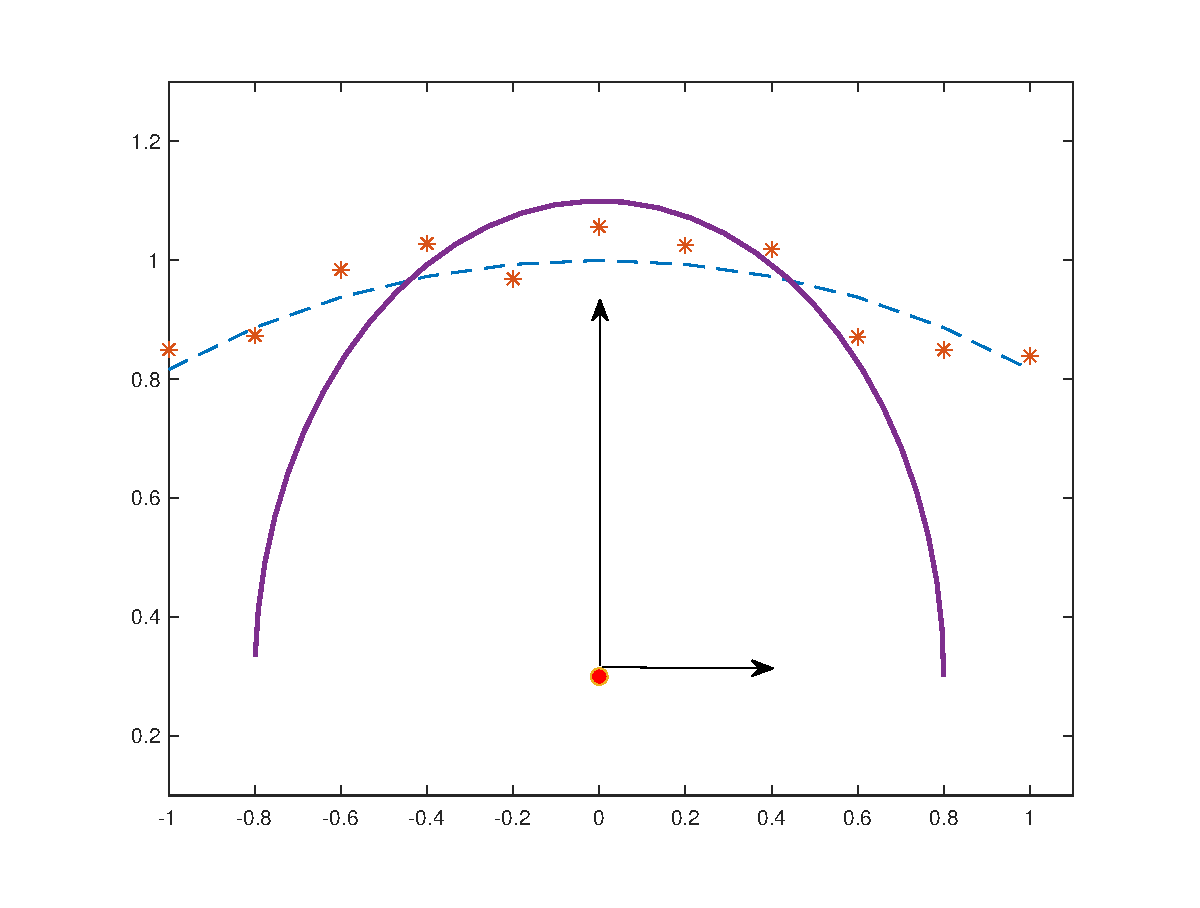
\includegraphics[width=0.32\linewidth]{../figures/demo1.eps} 
\hspace{-4mm}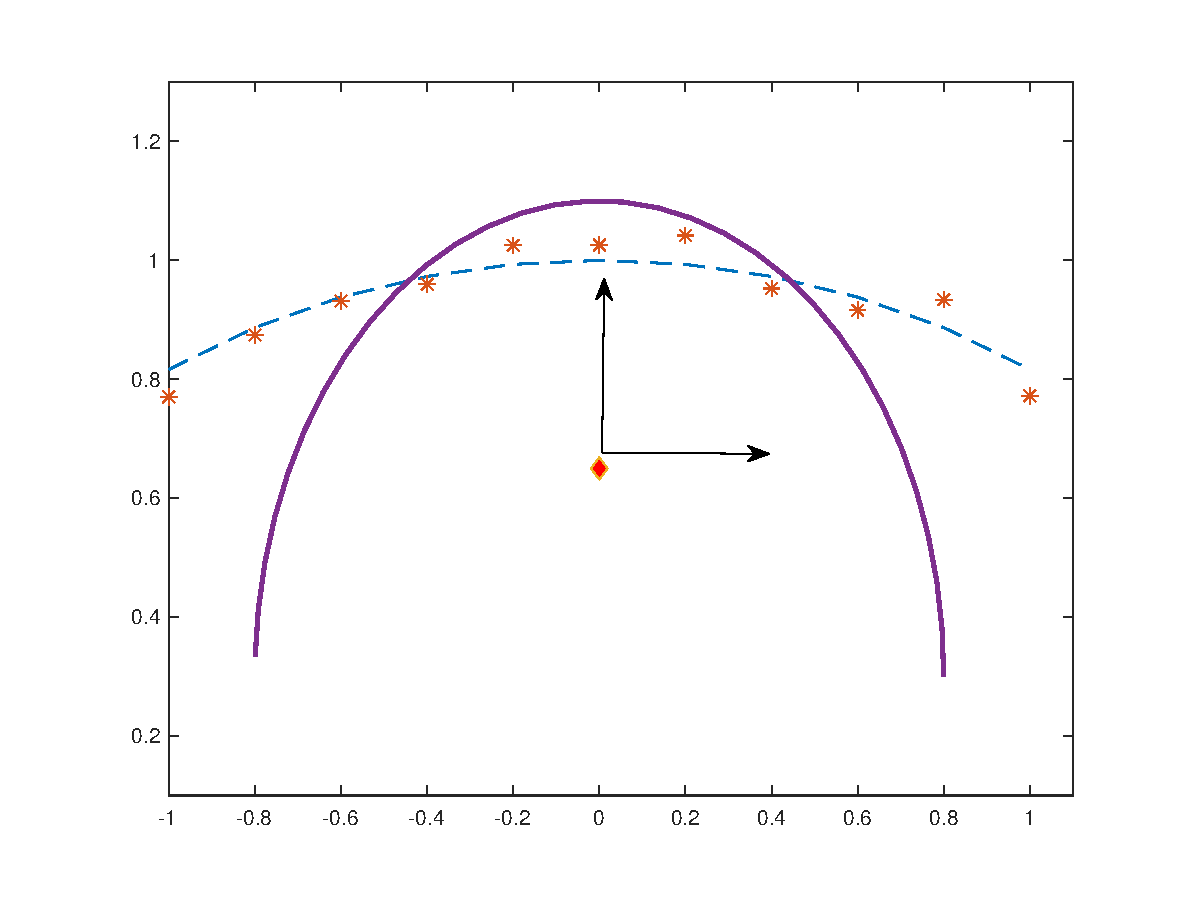
\includegraphics[width=0.32\linewidth]{../figures/demo2.eps} 
\hspace{-4mm}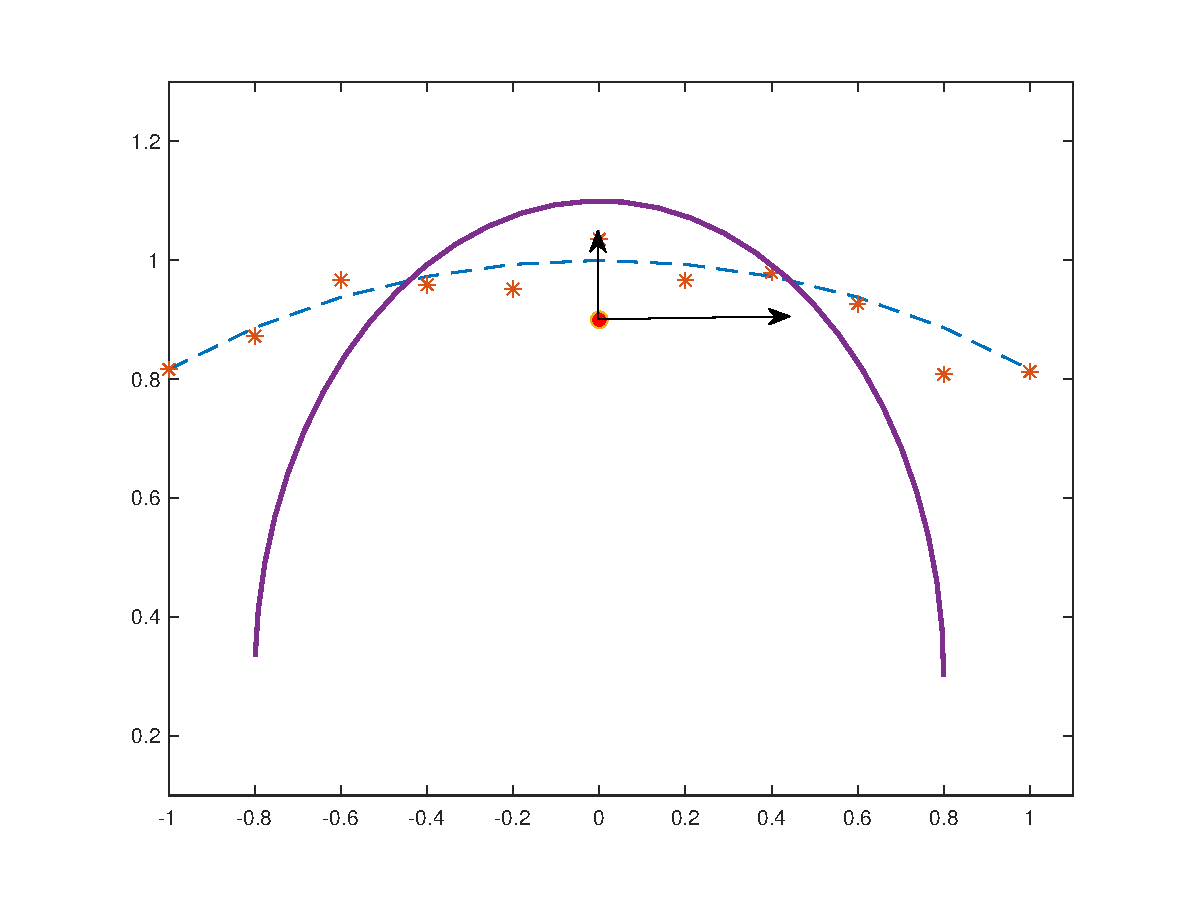
\includegraphics[width=0.32\linewidth]{../figures/demo3.eps} 
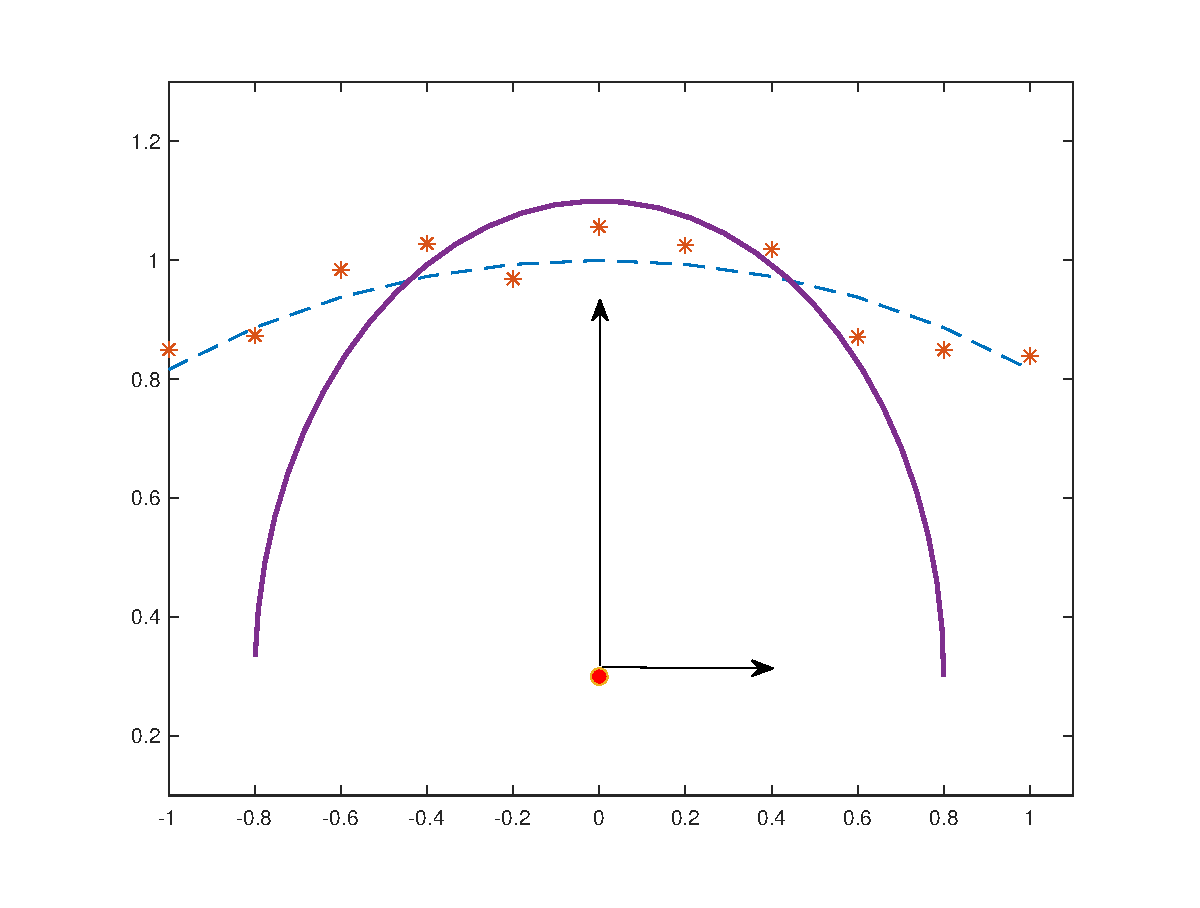
\includegraphics{../figures/demo1.eps}
%\setcaptionwidth{6in}
\caption{The process of $J(x)$'s eigenspace's variation with $x$ approaching the manifold }
\label{Shifting Eigenvectors}
\end{figure}

\begin{figure}
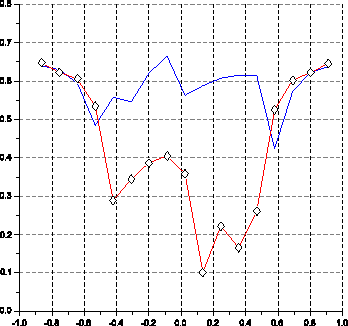
\includegraphics{figure1}
\caption{Pathway of the penicillin G biosynthesis.}
\label{penG}
\end{figure}

Sample of cross-reference to figure.
Figure~\ref{penG} shows that it is not easy to get something on paper.

\section{Equations and the like}

Two equations:
\begin{equation}
    C_{s}  =  K_{M} \frac{\mu/\mu_{x}}{1-\mu/\mu_{x}} \label{ccs}
\end{equation}
and
\begin{equation}
    G = \frac{P_{\mathrm{opt}} - P_{\mathrm{ref}}}{P_{\mathrm{ref}}}  100(\%).
\end{equation}

Equation arrays:
\begin{eqnarray}
  \frac{dS}{dt} & = & - \sigma X + s_{F} F,\\
  \frac{dX}{dt} & = &   \mu    X,\\
  \frac{dP}{dt} & = &   \pi    X - k_{h} P,\\
  \frac{dV}{dt} & = &   F.
\end{eqnarray}
One long equation:
\begin{eqnarray}
 \mu_{\text{normal}} & = & \mu_{x} \frac{C_{s}}{K_{x}C_{x}+C_{s}}  \nonumber\\
                     & = & \mu_{\text{normal}} - Y_{x/s}\bigl(1-H(C_{s})\bigr)(m_{s}+\pi /Y_{p/s})\\
                     & = & \mu_{\text{normal}}/Y_{x/s}+ H(C_{s}) (m_{s}+ \pi /Y_{p/s}).\nonumber
\end{eqnarray}
%%%%%%%%%%%%%%%%%%%%%%%%%%%%%%%%%%%%%%%%%%%%%%
%% Example with single Appendix:            %%
%%%%%%%%%%%%%%%%%%%%%%%%%%%%%%%%%%%%%%%%%%%%%%
\begin{appendix}
\section*{Title}\label{appn} %% if no title is needed, leave empty \section*{}.
Appendices should be provided in \verb|{appendix}| environment,
before Acknowledgements.

If there is only one appendix,
then please refer to it in text as \ldots\ in the \hyperref[appn]{Appendix}.
\end{appendix}
%%%%%%%%%%%%%%%%%%%%%%%%%%%%%%%%%%%%%%%%%%%%%%
%% Example with multiple Appendixes:        %%
%%%%%%%%%%%%%%%%%%%%%%%%%%%%%%%%%%%%%%%%%%%%%%
\begin{appendix}
\section{Title of the first appendix}\label{appA}
If there are more than one appendix, then please refer to it
as \ldots\ in Appendix \ref{appA}, Appendix \ref{appB}, etc.

\section{Title of the second appendix}\label{appB}
\subsection{First subsection of Appendix \protect\ref{appB}}

Use the standard \LaTeX\ commands for headings in \verb|{appendix}|.
Headings and other objects will be numbered automatically.
\begin{equation}
\mathcal{P}=(j_{k,1},j_{k,2},\dots,j_{k,m(k)}). \label{path}
\end{equation}

Sample of cross-reference to the formula (\ref{path}) in Appendix \ref{appB}.
\end{appendix}

%%%%%%%%%%%%%%%%%%%%%%%%%%%%%%%%%%%%%%%%%%%%%%
%% Support information (funding), if any,   %%
%% should be provided in the                %%
%% Acknowledgements section.                %%
%%%%%%%%%%%%%%%%%%%%%%%%%%%%%%%%%%%%%%%%%%%%%%
\section*{Acknowledgements}
The authors would like to thank the anonymous referees, an Associate
Editor and the Editor for their constructive comments that improved the
quality of this paper.

The first author was supported by NSF Grant DMS-??-??????.

The second author was supported in part by NIH Grant ???????????.


%%%%%%%%%%%%%%%%%%%%%%%%%%%%%%%%%%%%%%%%%%%%%%
%% Supplementary Material, if any, should   %%
%% be provided in {supplement} environment  %%
%% with title and short description.        %%
%%%%%%%%%%%%%%%%%%%%%%%%%%%%%%%%%%%%%%%%%%%%%%
\begin{supplement}
\textbf{Title of Supplement A}.
Short description of Supplement A.
\end{supplement}
\begin{supplement}
\textbf{Title of Supplement B}.
Short description of Supplement B.
\end{supplement}

%%%%%%%%%%%%%%%%%%%%%%%%%%%%%%%%%%%%%%%%%%%%%%%%%%%%%%%%%%%%%
%%                  The Bibliography                       %%
%%                                                         %%
%%  imsart-???.bst  will be used to                        %%
%%  create a .BBL file for submission.                     %%
%%                                                         %%
%%  Note that the displayed Bibliography will not          %%
%%  necessarily be rendered by Latex exactly as specified  %%
%%  in the online Instructions for Authors.                %%
%%                                                         %%
%%  MR numbers will be added by VTeX.                      %%
%%                                                         %%
%%  Use \cite{...} to cite references in text.             %%
%%                                                         %%
%%%%%%%%%%%%%%%%%%%%%%%%%%%%%%%%%%%%%%%%%%%%%%%%%%%%%%%%%%%%%

%% if your bibliography is in bibtex format, uncomment commands:
%\bibliographystyle{imsart-number} % Style BST file (imsart-number.bst or imsart-nameyear.bst)
%\bibliography{bibliography}       % Bibliography file (usually '*.bib')

%% or include bibliography directly:
\begin{thebibliography}{4}
%%
\bibitem{r1}
\textsc{Billingsley, P.} (1999). \textit{Convergence of
Probability Measures}, 2nd ed.
Wiley, New York.

\bibitem{r2}
\textsc{Bourbaki, N.}  (1966). \textit{General Topology}  \textbf{1}.
Addison--Wesley, Reading, MA.

\bibitem{r3}
\textsc{Ethier, S. N.} and \textsc{Kurtz, T. G.} (1985).
\textit{Markov Processes: Characterization and Convergence}.
Wiley, New York.

\bibitem{r4}
\textsc{Prokhorov, Yu.} (1956).
Convergence of random processes and limit theorems in probability
theory. \textit{Theory  Probab.  Appl.}
\textbf{1} 157--214.
\end{thebibliography}

\end{document}

